% !TEX root = /Users/Gela/Desktop/Thesis_latex/thesis.tex
\section{Modeling}
\label{sec:modres}
A physical model of the membrane was made and the given results can be seen below. In figure \ref{fig:simscape} the flowchart is given. The RO-membrane is simulated with three nodes; feed, product and reject, and an extra input for specifying the temperature. The temperature node gives freedom to simulate the behaviour of the membrane at different temperatures. \\
\\
The model consists of the pump, pipes, valves and a tank. The water in the tank can be set to contain any salt concentration to be able to simulate different conductivity values. The speed of the pumps can be changed to change the flow and pressure characteristic over the membrane in the model. \\
\\
All plots in this section show expected behaviour according to the theory about membrane behaviour when the temperature is rising. Flow and conductivity on permeate/product side are increasing which is desirable to control in the system, and to be kept at limited values in order to have the water device to handle these differences in working conditions. The results of the simulations are considered to be realistic according to the theory of the membrane. More details of the parameters in the model can be  seen in subsections below.\\
\\
\begin{figure}[h]
\label{fig:simscape}
\centering
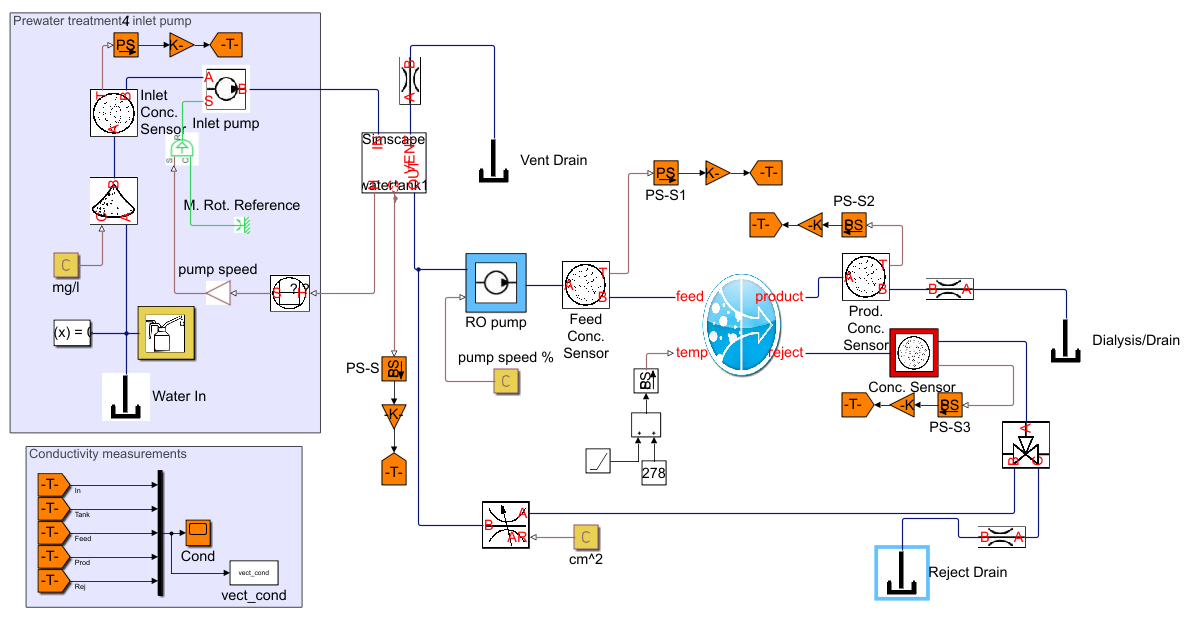
\includegraphics[width=\textwidth]{simscape_fc1.PNG}
\caption{Model made in Matlab tool Simscape }
\end{figure}
\newpage


\subsection{Temperature}
In figure \ref{fig:temp} the simulated temperature, 278-316 K is shown. Plots \ref{fig:tcf} - 6.11 show the behaviour over a simulated time of 2000 s and a temperature range of 278-316 K. Pump speed is kept constant. The temperature correction factor, $TCF$, in figure \ref{fig:tcf} is the temperature dependant parameter implemented in the simulated model to receive the differences of the behaviour of the membrane. At 298 K $TCF$ is equal to 1. Below and above it is adjusted to compensate for the differences of the membrane behaviour. 
\begin{figure}[h]
  \centering
  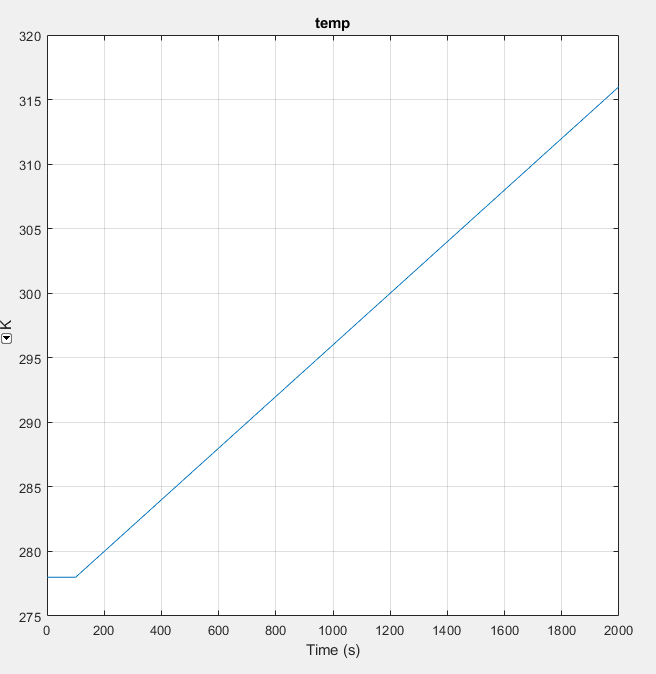
\includegraphics[width=0.6\linewidth]{temp.PNG}
  \caption{Temperature range in simulations, from 278-316 K}
  \label{fig:temp}
\end{figure}

\begin{figure}[h]
\centering
    \centering
    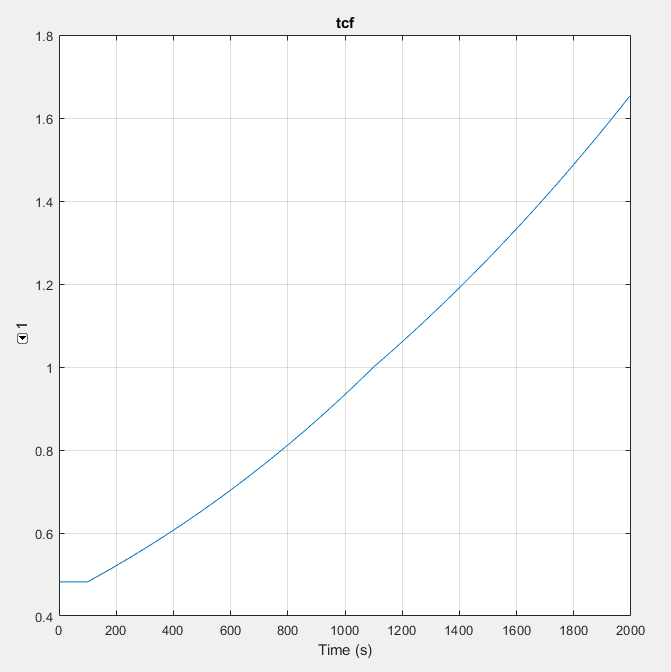
\includegraphics[width=0.6\textwidth]{tcf.PNG}
    \caption{Temperature correction factor, $TCF$, when temperature is simulated from 278-316 K}
    \label{fig:tcf}
\end{figure}
\newpage

\subsection{Salt concentration}
In figure \ref{fig:msaltf} the salt concentration in kg/s on the feed side of the membrane is shown. The salt concentration increases with increasing temperature. In figure \ref{fig:msaltp} the salt concentration in the product water is shown. Due to the mass balance equation in \ref{sec:soldiff} the sign is negative, and the concentration increases with temperature. Figure \ref{fig:msaltr} shows the salt concentration on the reject side. It increases a little with temperature (negative sign due to the mass balance equations).\\
The salt concentration in the feed water increases from 0.8 kg/s to 0.96 kg/s. The product water concentration increases from 0.2 to 1.8 kg/s. The reject salt concentration increases from 0.8 to 0.96 kg/s.\\
\\
The salt concentration characteristics is in line with the expected values of the system for the simulations and is considered to be realistic for the model. 
\begin{figure}[H]
\centering
    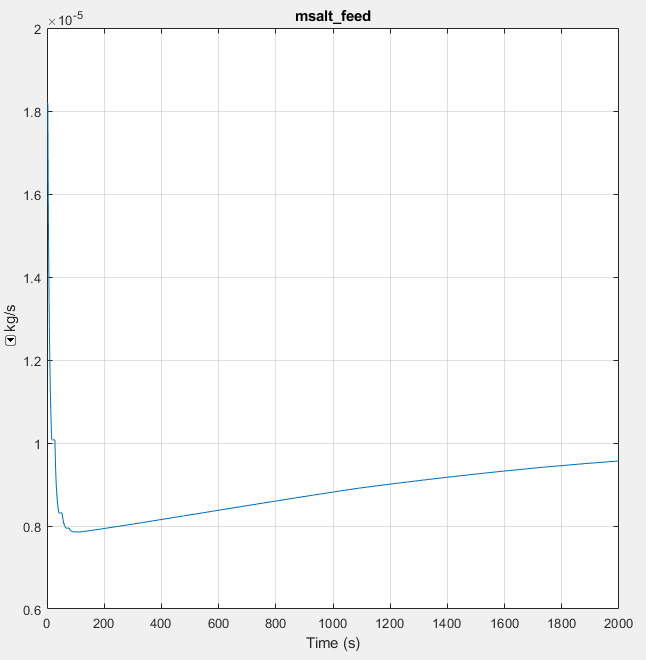
\includegraphics[width=0.6\textwidth]{msalt_feed.PNG}
    \caption{Salt concentration in feed water, when temperature is simulated from 278-316 K}
    \label{fig:msaltf}
\end{figure}

\begin{figure}[H]
\centering
  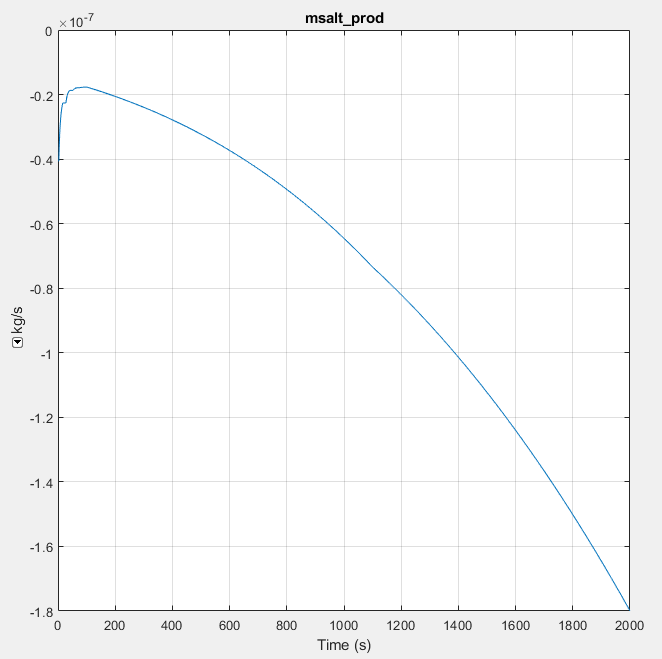
\includegraphics[width=0.6\linewidth]{msalt_prod.PNG}
  \caption{Salt concentration in product water, when temperature is simulated from 278-316 K}
  \label{fig:msaltp}
\end{figure}

\begin{figure}[H]
  \centering
  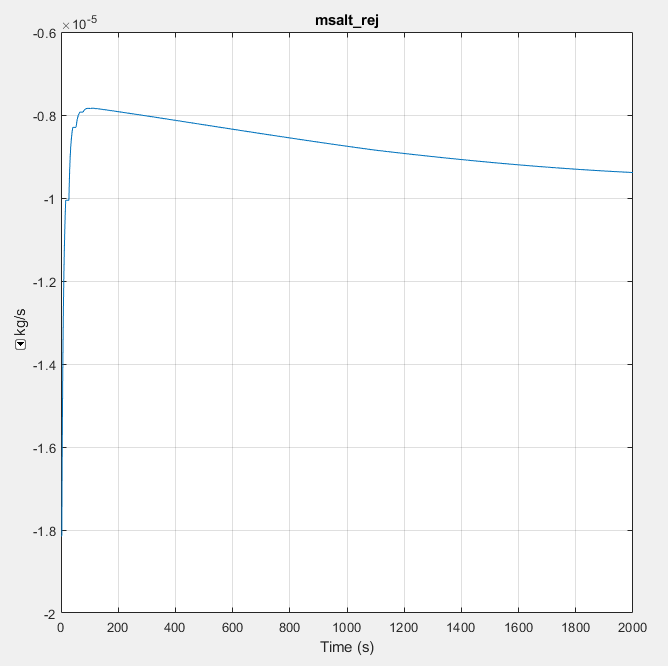
\includegraphics[width=0.6\linewidth]{msalt_rej.PNG}
  \caption{Salt concentration in reject water, when temperature is simulated from 278-316 K}
  \label{fig:msaltr}
\end{figure}
\newpage
\newpage

\subsection{Flow}
Figure \ref{fig:qf} - \ref{fig:qrej} show the flow in the three nodes; feed, product and reject. The mass balance equation in \ref{sec:soldiff} gives negative sign on reject and product side. The feed water flow increases negligible from 8.441-8.444 l/min. Product/permeate water flow increases from (-) 0.62-1.42 l/min. Reject water flow decreases from (-) 7.82-7.2 l/min. \\
\\
The plots show expected behaviour of the flow in the system. The membrane pore size is increasing with temperature and the permeate flow is increasing with rising temperature.
\begin{figure}[H]
  \centering
  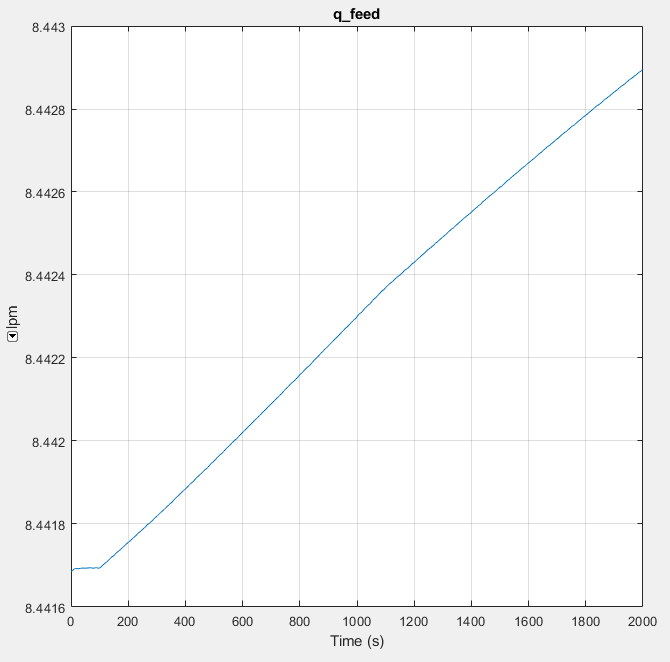
\includegraphics[width=0.6\linewidth]{q_feed.PNG}
  \caption{Flow feed side, when temperature is simulated from 278-316 K}
  \label{fig:qf}
\end{figure}
\begin{figure}[H]
  \centering
  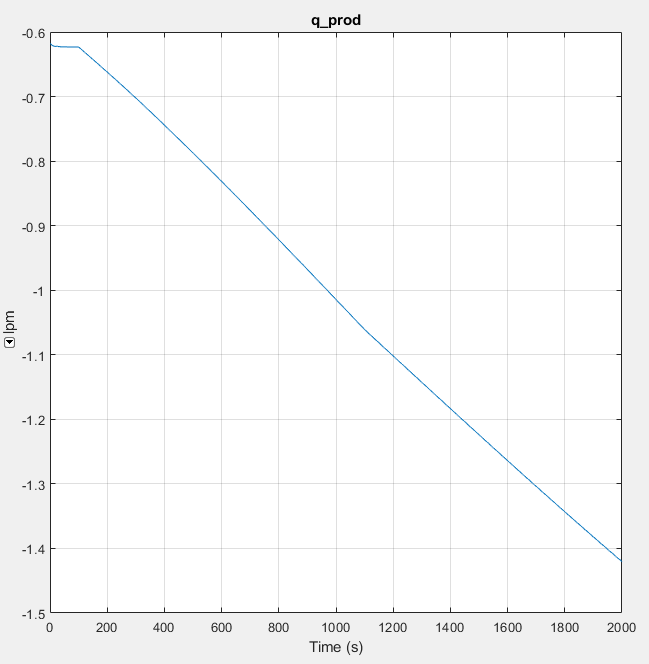
\includegraphics[width=0.6\linewidth]{q_prod.PNG}
  \caption{Flow product side, when temperature is simulated from 278-316 K}
  \label{fig:qp}
\end{figure}
\begin{figure}[H]
  \centering
  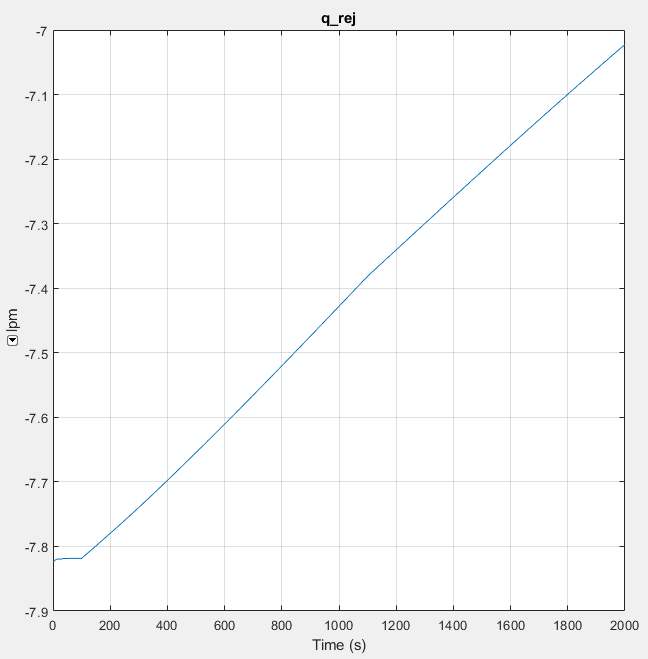
\includegraphics[width=0.6\linewidth]{q_rej.PNG}
  \caption{Flow reject side, when temperature is simulated from 278-316 K}
  \label{fig:qrej}
\end{figure}
\newpage

\subsection{Pressure}
Figure \ref{fig:deltap} shows pressure difference from feed side to product side. The pressure decreases from (-) 11.5-7.7 bar when temperature changes from 278-316 K which is expected when temperature is rising. This is due to the temperature dependency of the membrane. When temperature is rising, the membrane pore size is increasing and let more water flow through the membrane which contributes with the lower pressure. \\
\\
\begin{figure}[H]
  \centering
  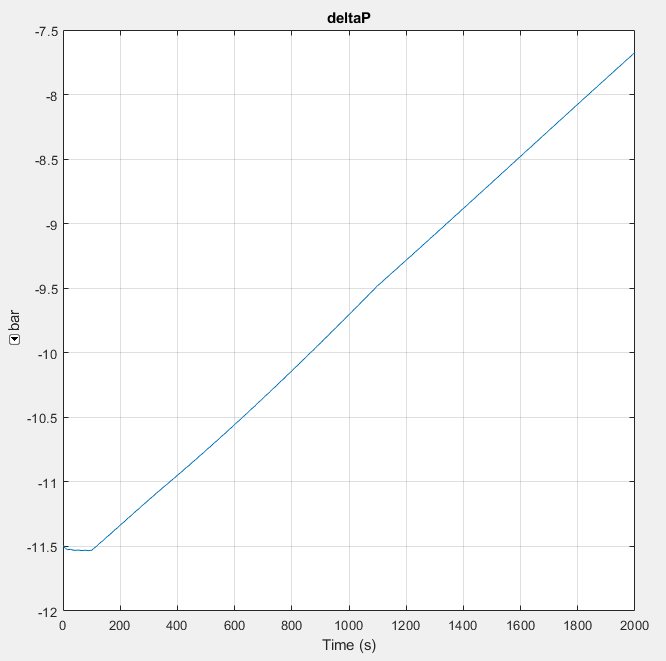
\includegraphics[width=0.7\linewidth]{deltap.PNG}
  \caption{Pressure drop feed side to product side, when temperature is simulated from 278-316 K}
  \label{fig:deltap}
\end{figure}
\newpage

\subsection{Conductivity}
Figure \ref{fig:conden} displays the conductivity in feed, product and reject side. The conductivity in all nodes increases during the simulation. \\
\\
\begin{figure}[H]
  \label{fig:conden}
  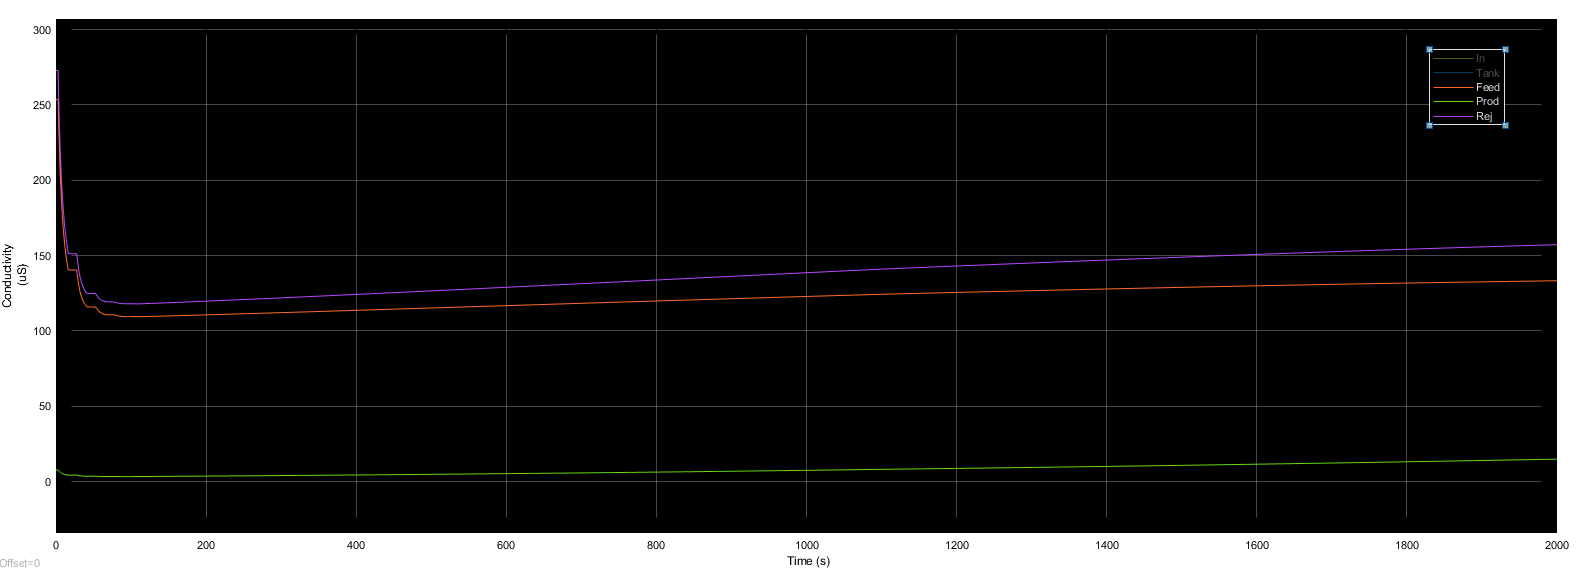
\includegraphics[width=1.1\linewidth]{cond.PNG}
  \caption{Conductivity in feed, reject and product side, when temperature is simulated from 278-316 K}
\end{figure}
\newpage


\section{Flowchart investigation}
By changing the flow path in the test setup both the one pump system and two pump system could be investigated and their performance could be compared. Both systems were considered fulfilling most of the requirements, section \ref{framing}, for an updated version. \\
\\
The one pump system, seen in figure \ref{fig:FlowCInves1}, was designed to use both a tank and the recirculation loop as a water source and to create pressure by generating a large flow over the membrane and recirculation restrictor with the pump implemented. The pump creates the flow, and together with the needle valve in the recirculation path the pressure over the membrane.  \\
\\
In the two pump system, seen in figure \ref{fig:Sys2}, the water path was modified so that the feed pump only used a tank as a source and pressurised the entire recirculation loop. The recirculation pump was installed instead of the needle valve used in the recirculation path. The pump was used to create the necessary flow within the recirculation loop.\\
\\
Two ideas of the two pump system were considered and the system with one pump in recirculation path was chosen. The big disadvantage with the implementation of a pump on the permeate side was that it might contaminate the permeate stream. Therefore, System 1 was precluded and System 2 with one pump on the feed side and one in the recirculation loop was chosen.\\
\\
An overview of the systems compared in this report can be seen below.\\
\begin{figure}[h]
\centering
\begin{minipage}{.5\textwidth}
    \centering
    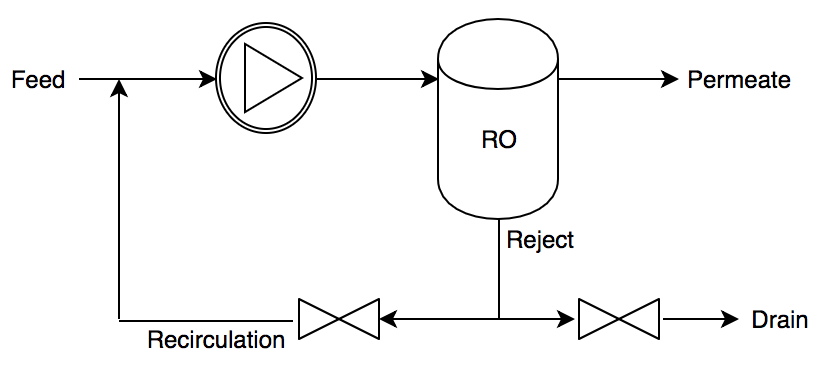
\includegraphics[width=1\textwidth]{Sys1}
    \caption{One pump system, as the current setup used in the water device today}
    \label{fig:System1}
\end{minipage}%
\begin{minipage}{.5\textwidth}
  \centering
  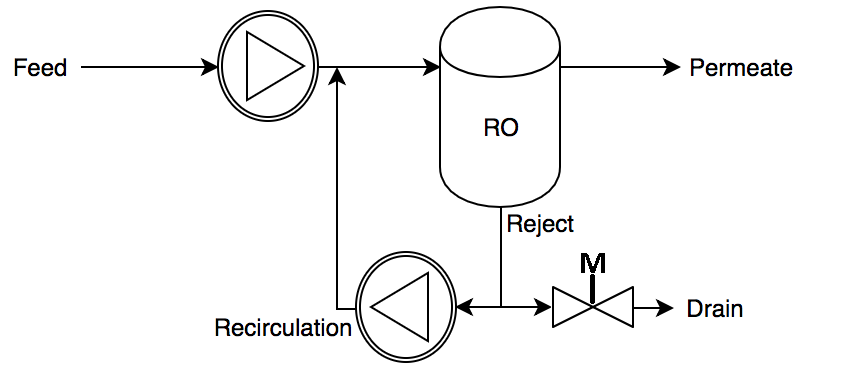
\includegraphics[width=1\linewidth]{Sys2}
  \caption{Two pump system, with one pump on feed side and one pump in the recirculation loop}
  \label{fig:System2}
\end{minipage}
\end{figure}

\newpage

\section{Flow monitoring using the pumps}
The mapping of the pumps RPM and flow rate can be seen in \ref{fig:RPM} and \ref{fig:Flowrate}.
\begin{figure}[H]
    \centering
    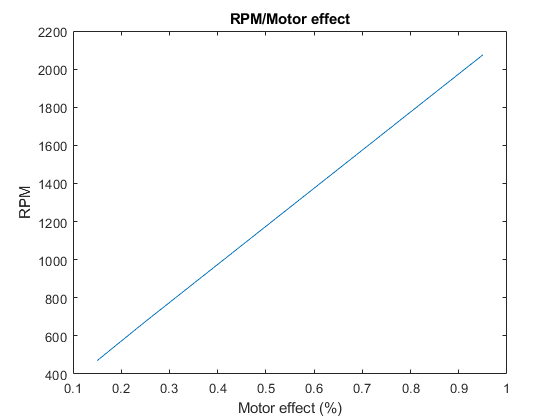
\includegraphics[width=0.5\textwidth]{RPM.png}
    \caption{RPM of the Pumps at different control signals/duty cycles}
    \label{fig:RPM}
\end{figure}
The RPM was measured by the hall sensor in the pump. The flow rate was calculated by investigating the flow at different RPMs and outlet pressures. From the gathered data it was possible to calculate the flow at any given RPM in real-time. This could then be used by the simulink program to measure the flow in the system at any given time.  
\begin{figure}[H]
    \centering
    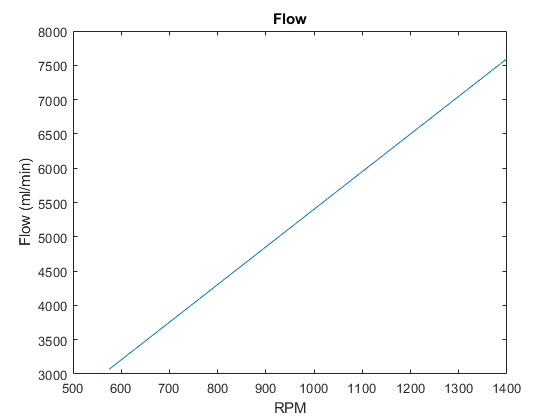
\includegraphics[width=0.5\textwidth]{Flow.png}
    \caption{Flow rate at different control signals/duty cycles}
    \label{fig:Flowrate}
\end{figure}

\newpage
\section{Building the test rig}
A test rig was built to be able to investigate the performance of both the one pump system and the two pump system. Initially, the one pump system was implemented and once all the testing on that system had been completed the flow path was changed according to \ref{fig:Sys2}.\\
\\
The biggest challenge when building the rig was the high pressure on the feed side of the membrane. It was difficult to find components that would be able to function up to 15 bar and the solution was to modify sensors used in old prototype machines. A sensor block that was able to measure temperature, conductivity and pressure at high pressure was built and can be seen in figure \ref{fig:Rig1} (the rectangular blocks in the feed, reject and permeate stream). The hall sensors in the pumps were used to measure the flow in the pressurized parts of the system and a standard flow sensor was used to measure the permeate flow. A motorized valve was used as a drain valve, this valve can be seen in figure \ref{fig:Rig1} (bottom right)\\
\\
The full system setup can be seen in figure \ref{fig:Rig2}. The computer to the left displays the control GUI and the simulink program. The heating bath was located in front of the rig. The display to the right was connected to the real time target computer and display important system information in real time.\\
\\
Safety systems were implemented to immediately shut down the rig if the pressure reached above 12 bar. This system was very useful not to accidentally destroy the system. The back side of the rig was also covered in plastic sheets not to allow a water leakage to reach the power supplies.\\
\\


\begin{figure}[H]
    \centering
    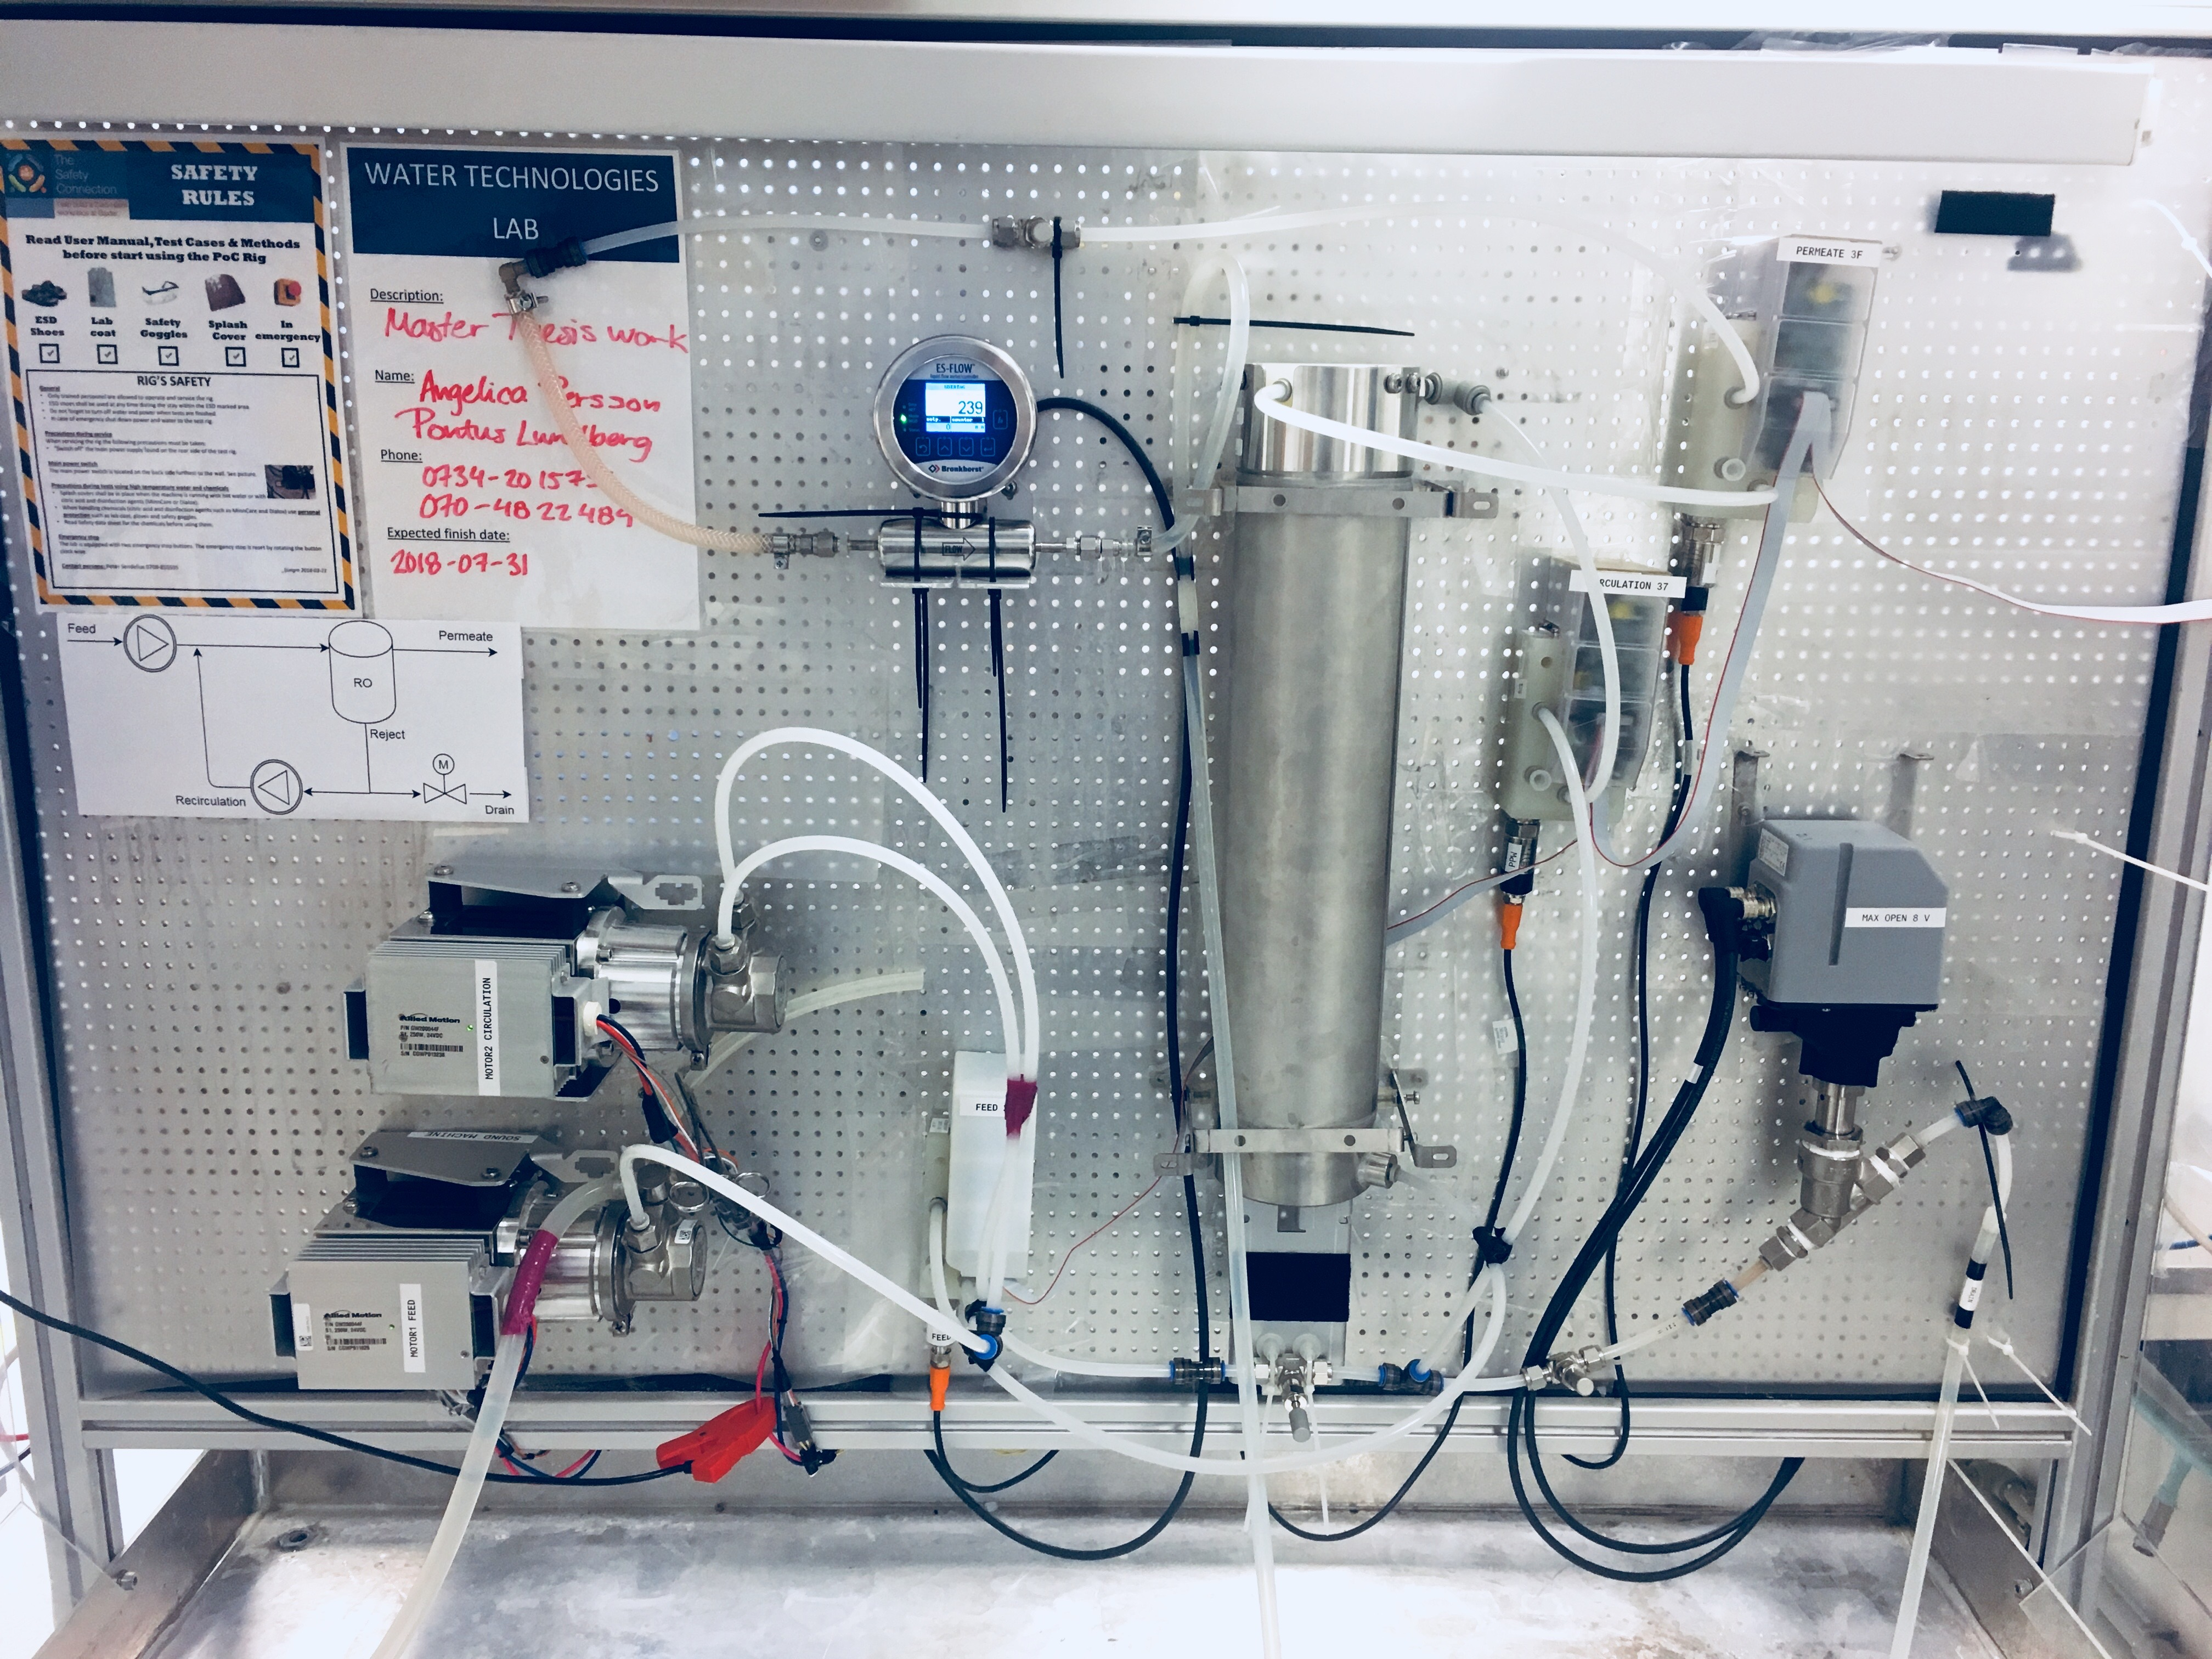
\includegraphics[width=1\textwidth]{Rig1}
    \caption{The rig built at Baxter Lund AB, with RO-membrane, pumps, pipes, flowmeter, measurement sensors and valves.}
    \label{fig:Rig1}
\end{figure}
\begin{figure}[H]
    \centering
    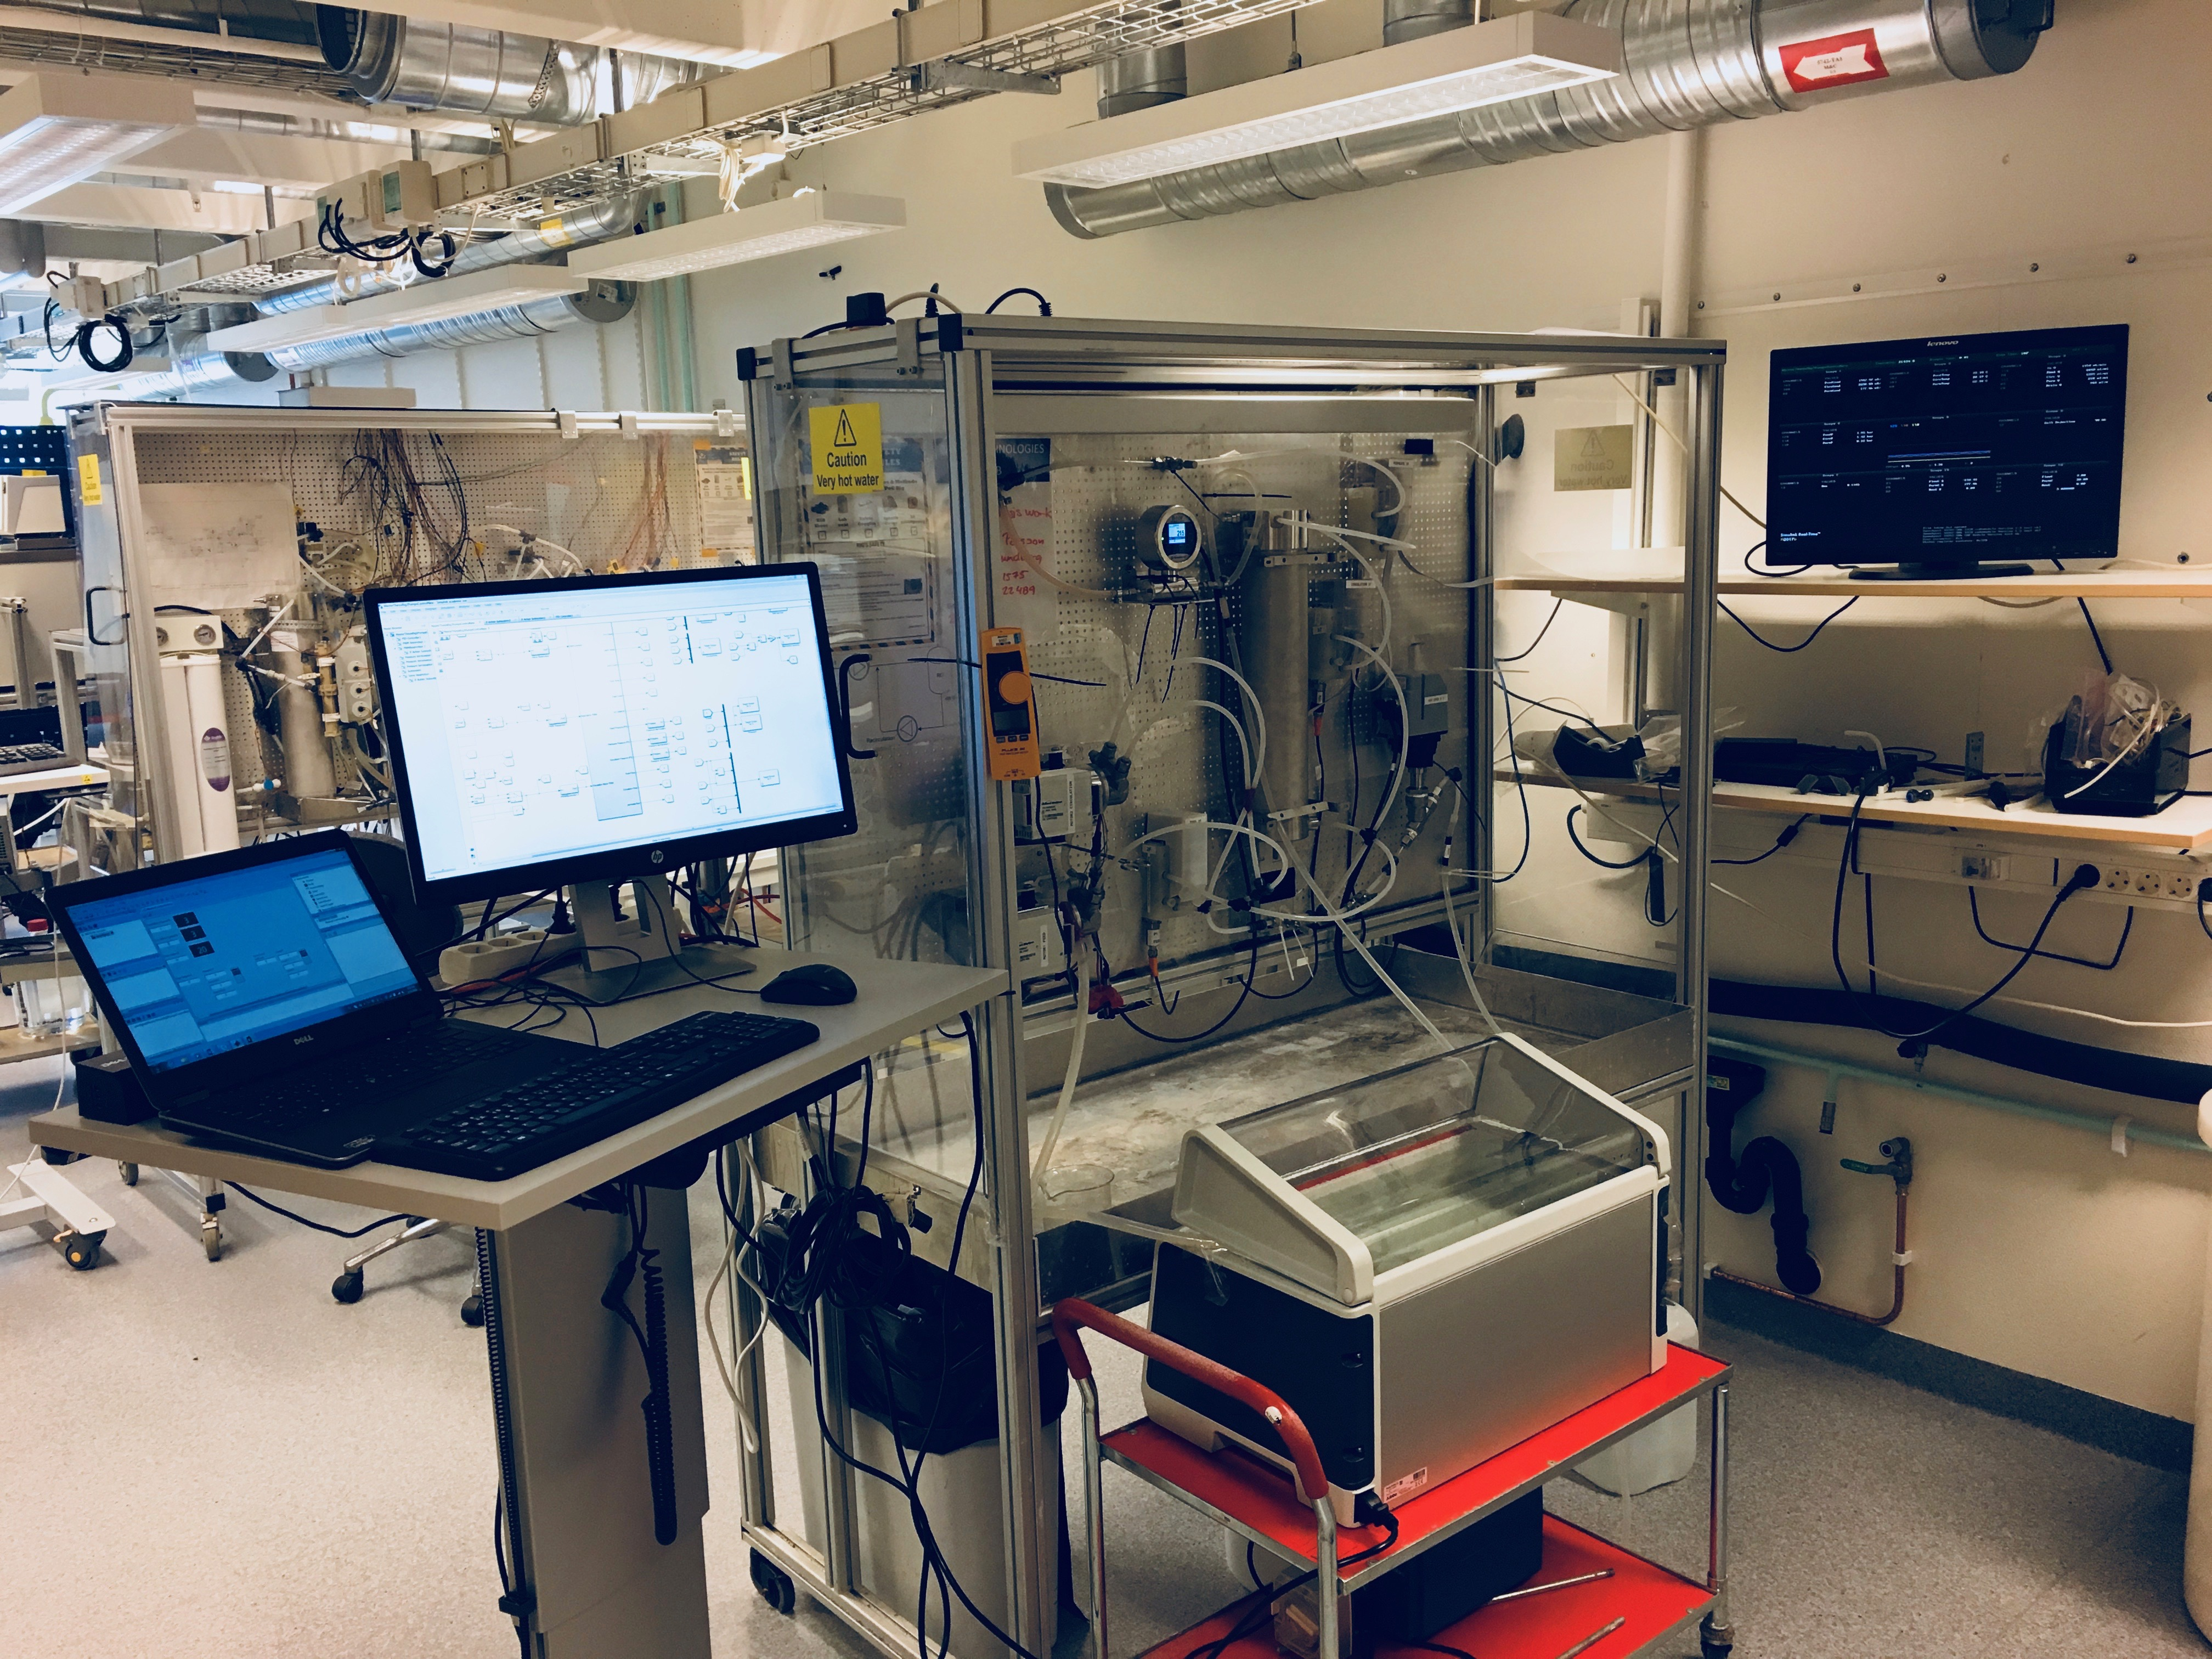
\includegraphics[width=1\textwidth]{Rig2}
    \caption{The full setup built at Baxter Lund AB, with Simulink implementation, GUI, display and water bath.}
    \label{fig:Rig2}
\end{figure}
\begin{figure}[H]
    \centering
    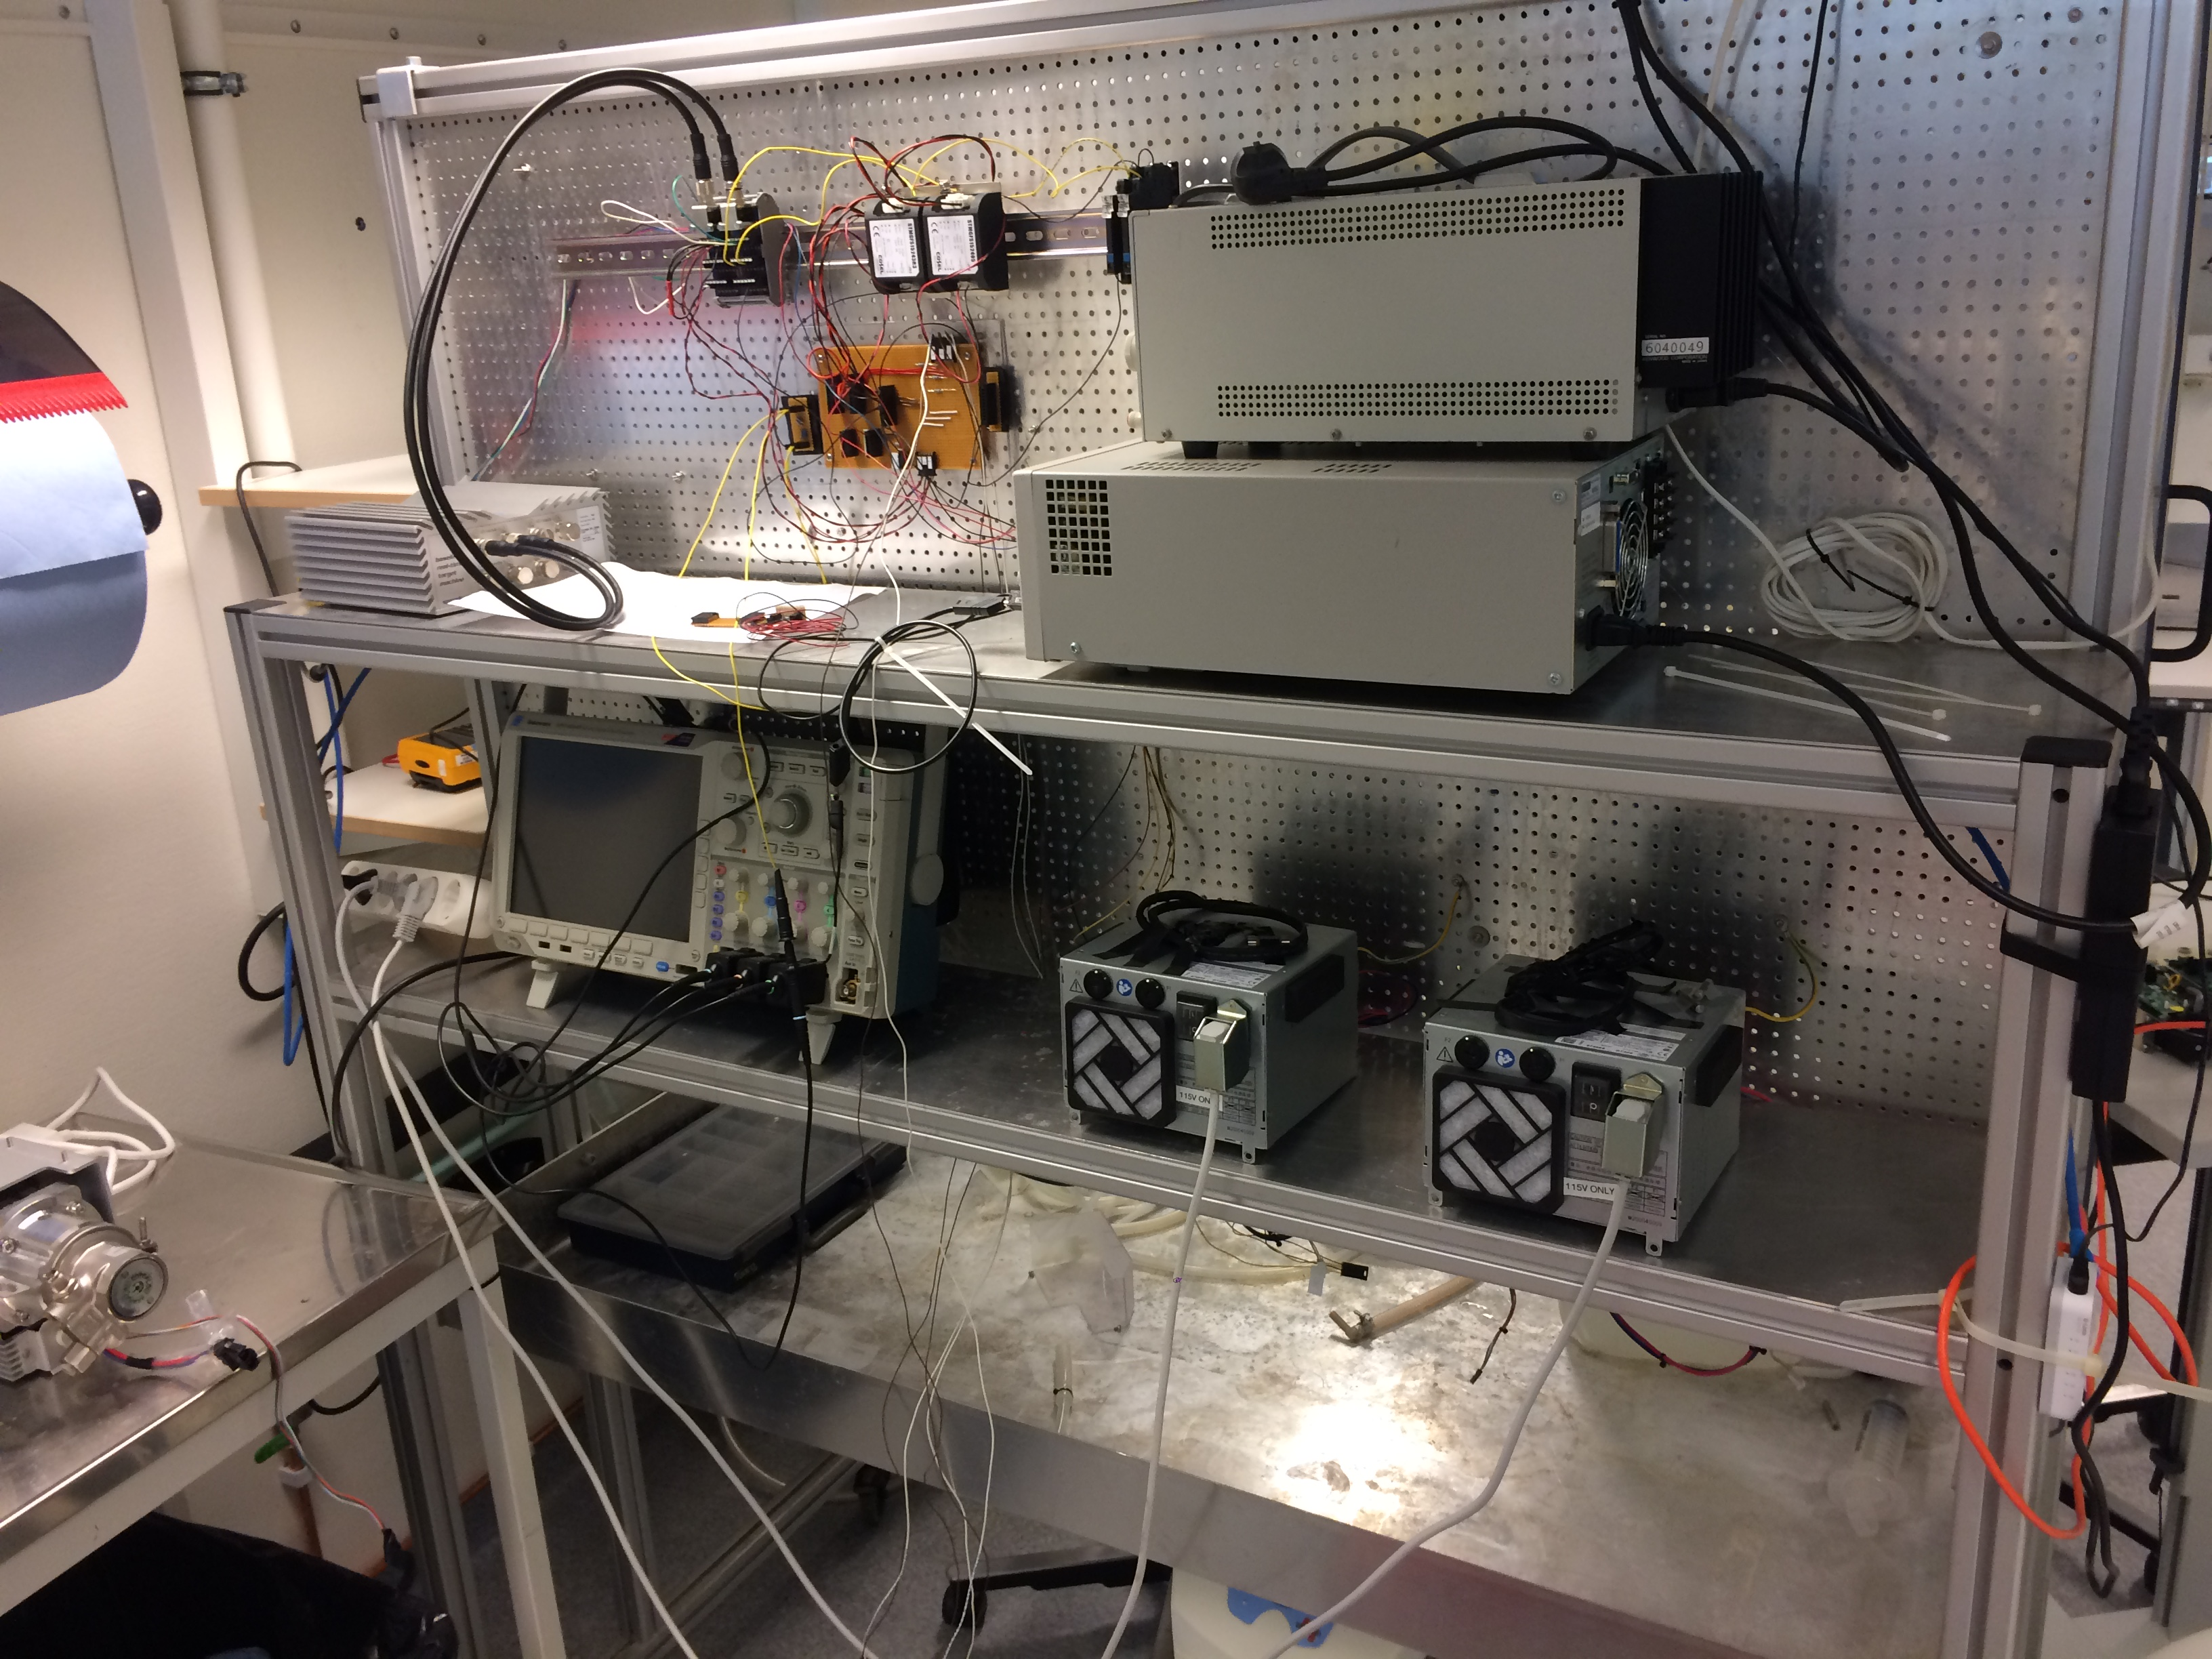
\includegraphics[width=1\textwidth]{back}
    \caption{Back side of the rig, top shelf: Speedgoat, power supplies and electronics to measure the sensors and control the motors and drain valve. Bottom shelf: power supplies connected to the motors.}
    \label{fig:back}
\end{figure}
\newpage
\subsection{Connections}
The electrical connections in the rig was done according to \ref{fig:PressConn} - \ref{fig:PumpConn}. Figure \ref{fig:display} and \ref{fig:gui} show the GUI and the real-time data display screen from the rig.  

\begin{figure}[H]
    \centering
    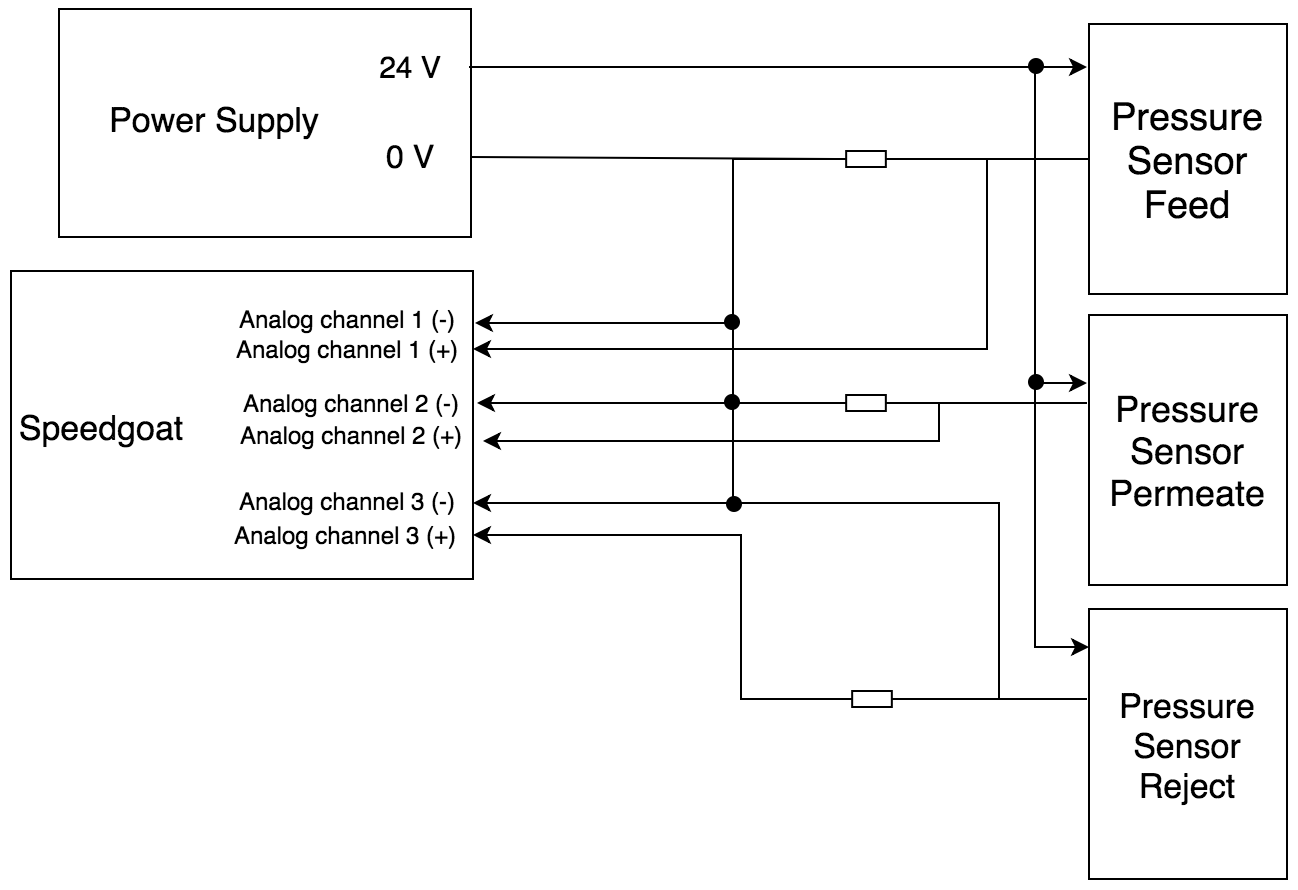
\includegraphics[width=0.6\textwidth]{PressConn}
    \caption{Connections Pressure sensors}
    \label{fig:PressConn}
\end{figure}
\begin{figure}[H]
    \centering
    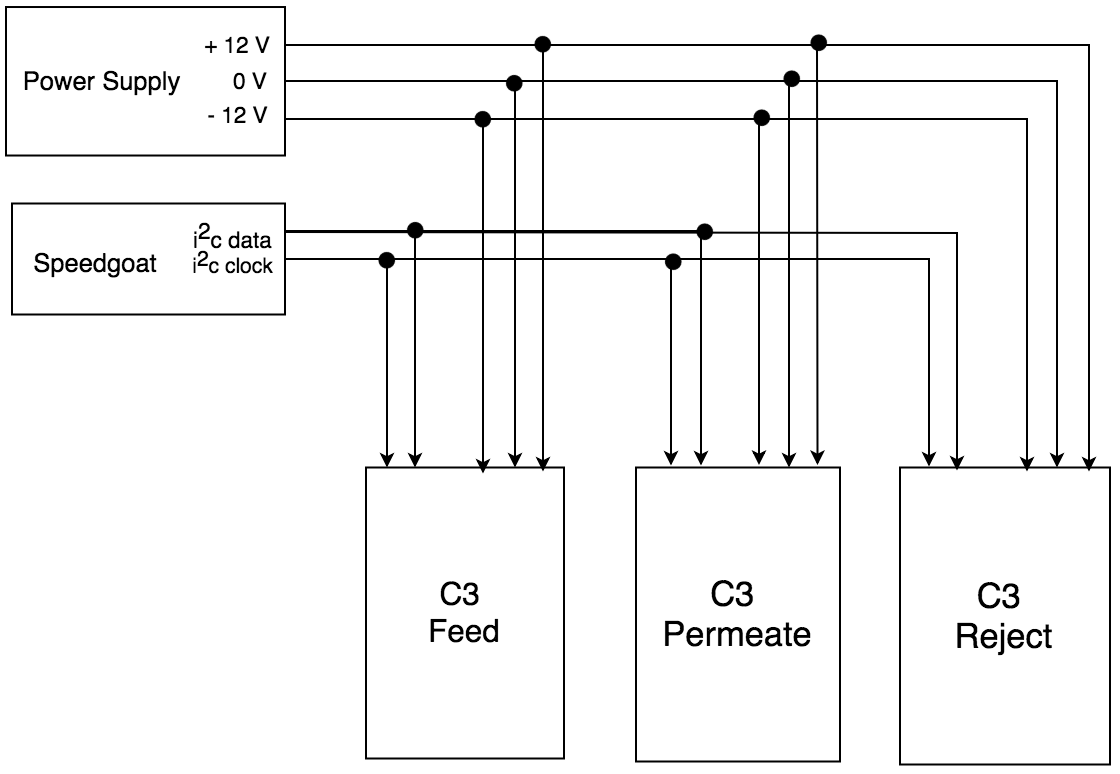
\includegraphics[width=0.6\textwidth]{C3Conn}
    \caption{Connections measurement blocks, C3}
    \label{fig:C3Conn}
\end{figure}
\begin{figure}[H]
    \centering
    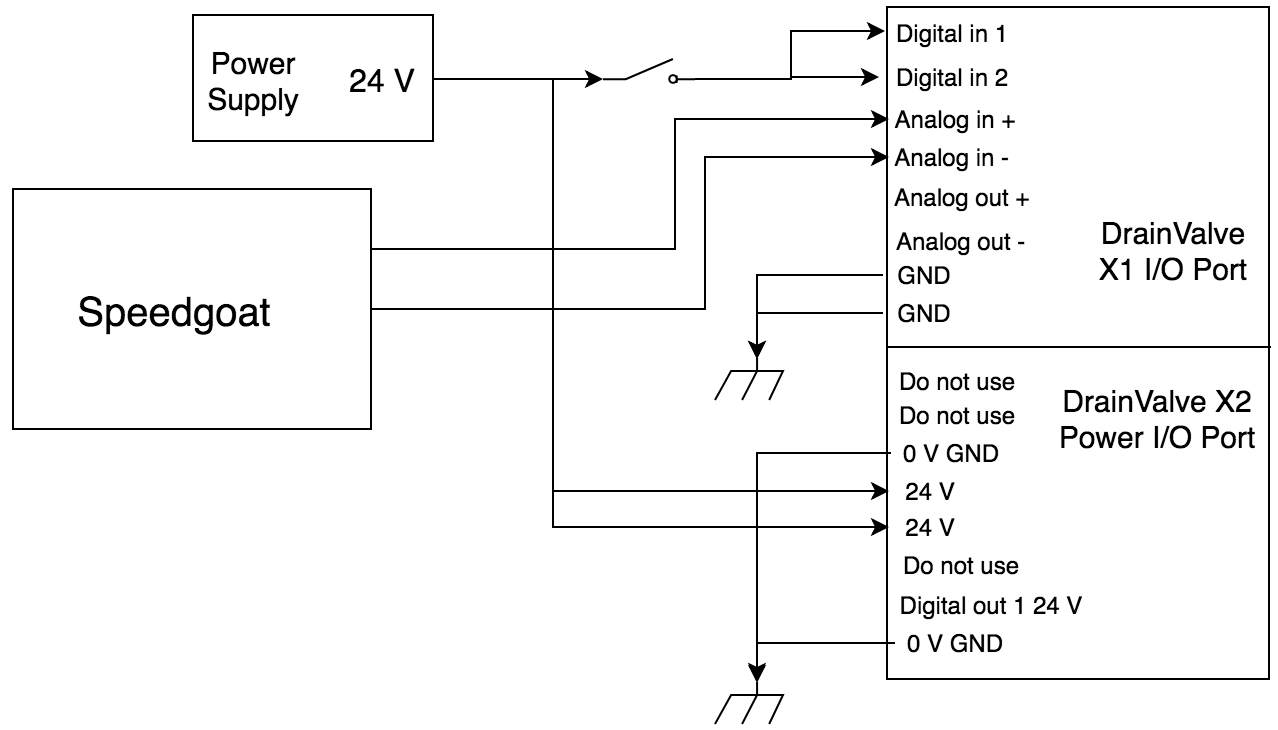
\includegraphics[width=0.6\textwidth]{ValveConn}
    \caption{Connections Drain Valve}
    \label{fig:ValveConn}
\end{figure}
\begin{figure}[H]
    \centering
    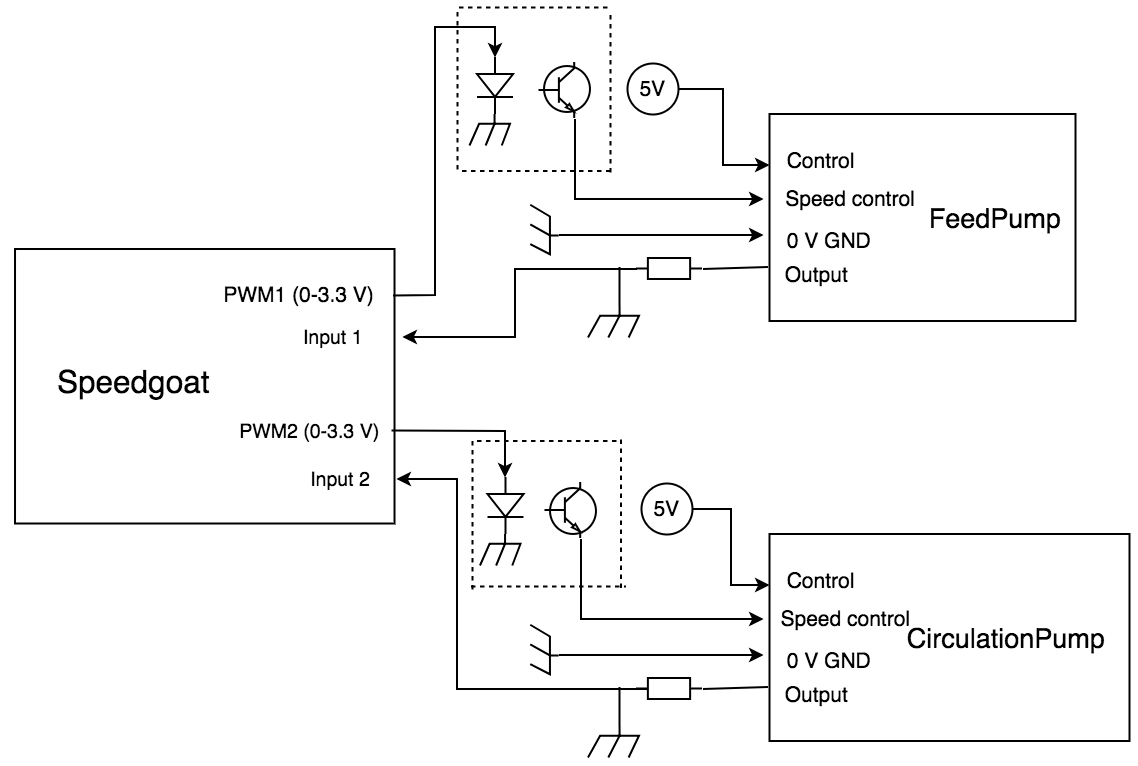
\includegraphics[width=0.6\textwidth]{PumpConn}
    \caption{Connections Pumps}
    \label{fig:PumpConn}
\end{figure}
\begin{figure}[H]
    \centering
    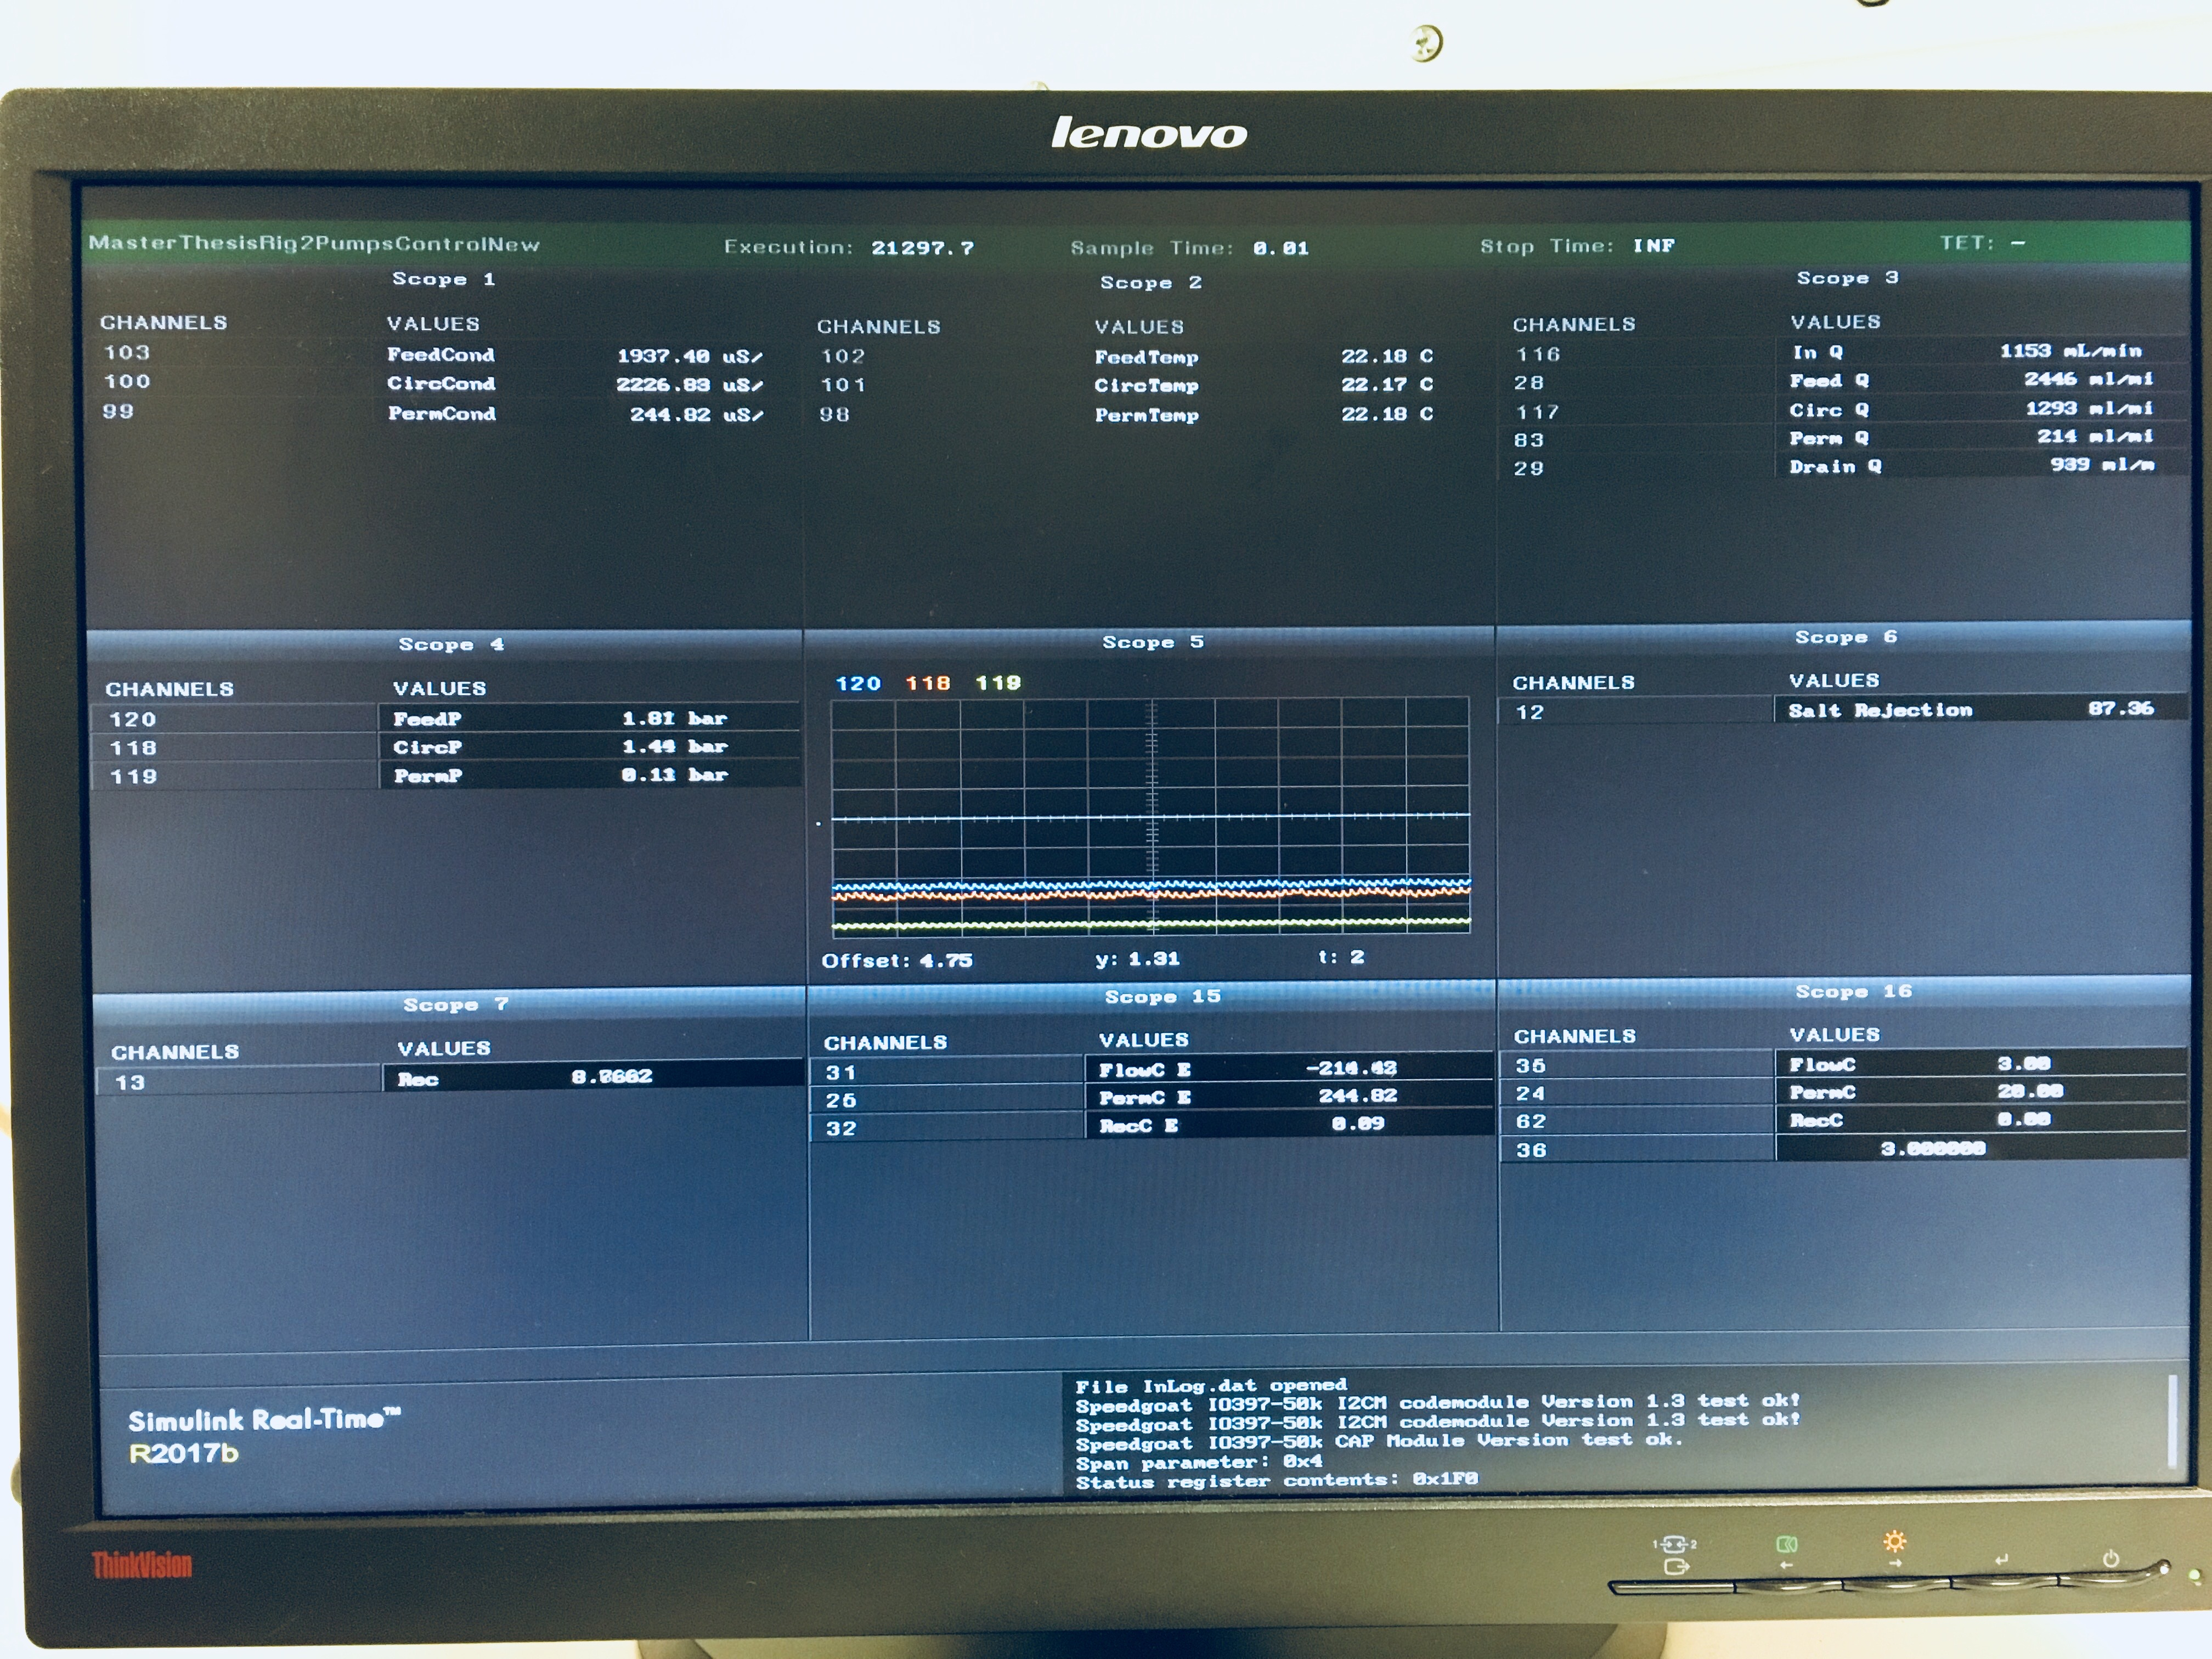
\includegraphics[width=0.9\textwidth]{Display}
    \caption{The Display showing rig data in real-time.}
    \label{fig:display}
\end{figure}
\begin{figure}[H]
    \centering
    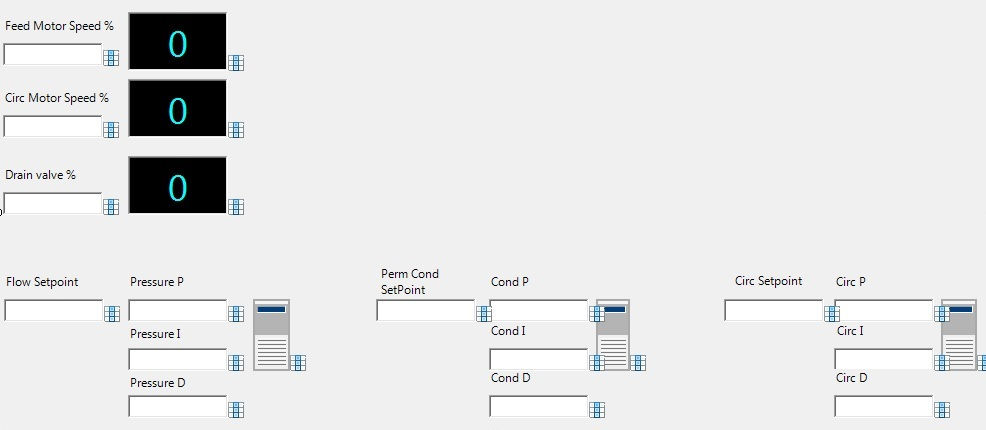
\includegraphics[width=0.9\textwidth]{GUI}
    \caption{The GUI implemented in Simulink to control the rig.}
    \label{fig:gui}
\end{figure}


\newpage


\section{Investigation of membrane behaviour}

In order to compare the two systems and understand how the membrane performed in different working conditions both systems needed to be tested. The tests were conducted by controlling the temperature, pumps and the conductivity in the recirculation loop and log how the different conditions affected the system and the membrane. The current one pump system was tested first.
\begin{figure}[H]
  \centering
    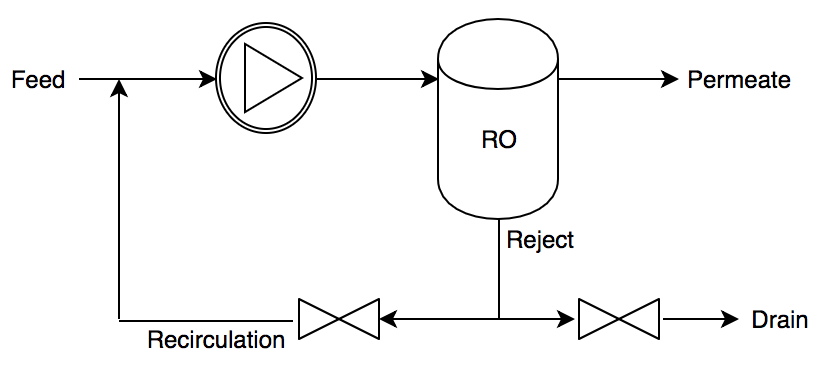
\includegraphics[width=0.8\textwidth]{Sys1}
    \caption{One pump system, the current setup used in the Water Device today}
    \label{fig:System1}
\end{figure}

The tests were conducted by changing the temperature, recirculation conductivity and pump speed and measure how the system behaved once it had reached steady state. The tests were divided into three test sequences. One test sequence was performed with room temperatured water (20  $^{\circ}$C), one with water heated to 30  $^{\circ}$C and in the last test sequence the water was heated to 40  $^{\circ}$C. Every test sequence included data from 8 steady state points with different settings on feed conductivity and pump speed. The test sequences are displayed in the table below. Each case represents one steady state point were data of the membrane behaviour was collected. 

Data collected:

\begin{itemize}
\item Pressure (bar): feed, reject and permeate
\item Flow (ml/min): feed, reject, permeate and drain
\item Conductivity (\SI{}{\micro\siemens}/cm): inlet, feed, reject and permeate
\item Temperature ($^\circ$C): feed, reject and permeate
\end{itemize}

From this, key values the following system parameters were calculated: net driving pressure, permeate flow, salt rejection, recovery, water efficiency and permeate conductivity. Table  \ref{tab:test cases} contains the tests planned for the system.

\newpage

\begin{table}[H]
\centering
\begin{tabular}{|p{1.4cm}||p{2cm}|p{3.2cm}|p{1.8cm}|}
 \hline
 \textbf{Steady state }&Temperature  ($^{\circ}$C)&Feed Conductivity (\SI{}{\micro\siemens}/cm)&Motor effect (\%) \\
 \hline
 1.1 & 20 & 280  & 60 \\
 1.2 & 20 & 500  & 60 \\
 1.3 & 20 & 1000 & 60  \\
 1.4 & 20 & 1000 & \textbf{80} \\
 1.5 & 20 & 2000 & 60 \\
 1.6 & 20 & 2000 & \textbf{80}\\
 1.7 & 20 & 3000 & 60 \\
 1.8 & 20 & 3000 & \textbf{80}\\
 \hline
 2.1 & 30 & 280 & 60 \\
 2.2 & 30 & 500 & 60 \\
 2.3 & 30 & 1000 & 60 \\
 2.4 & 30 & 1000 & \textbf{80}\\
 2.5 & 30 & 2000 & 60 \\
 2.6 & 30 & 2000 & \textbf{80}\\
 2.7 & 30 & 3000 & 60 \\
 2.8 & 30 & 3000 & \textbf{80}\\
 \hline 
 3.1 & 40 & 280 & 60 \\
 3.2 & 40 & 500 & 60 \\
 3.3 & 40 & 1000 & 60 \\
 3.4 & 40 & 1000 & \textbf{80}\\
 3.5 & 40 & 2000 & 60 \\
 3.6 & 40 & 2000 & \textbf{80}\\
 3.7 & 40 & 3000 & 60 \\
 3.8 & 40 & 3000 & \textbf{80}\\
\hline
\end{tabular}
\caption{Testcases for the investigations of the membrane behaviour. Each case represents one steady state in the experiments.}
    \label{tab:test cases} 
\end{table}


\newpage

\subsection{Current system, Test sequence 1, part 1}

The water tank was heated by the ambient temperature in the room while the test was running. Because of this, the test was split up in two parts, first the motor was set to 60\% and steady state 1.1, 1.2, 1.3, 1.5 and 1.7 were investigated. In the part 2, the motor was set to 80 \% and steady state 1.4, 1.6 and 1.8 were investigated. Figure \ref{fig:SteadyStates20C_1} and  \ref{fig:SteadyStates20C_2} show an overview of the tests at 20 $^{\circ}$C. The parts of the curves that have been marked with black are the steady state points. To be able to get good measurements an average was calculated from these marked values. Note that the three subplots within figure  \ref{fig:SteadyStates20C_1} and  \ref{fig:SteadyStates20C_2} share the same timeline so that the marked areas in all three plots are different measurements collected simulataneously.

\begin{figure}[h]
    \centering
    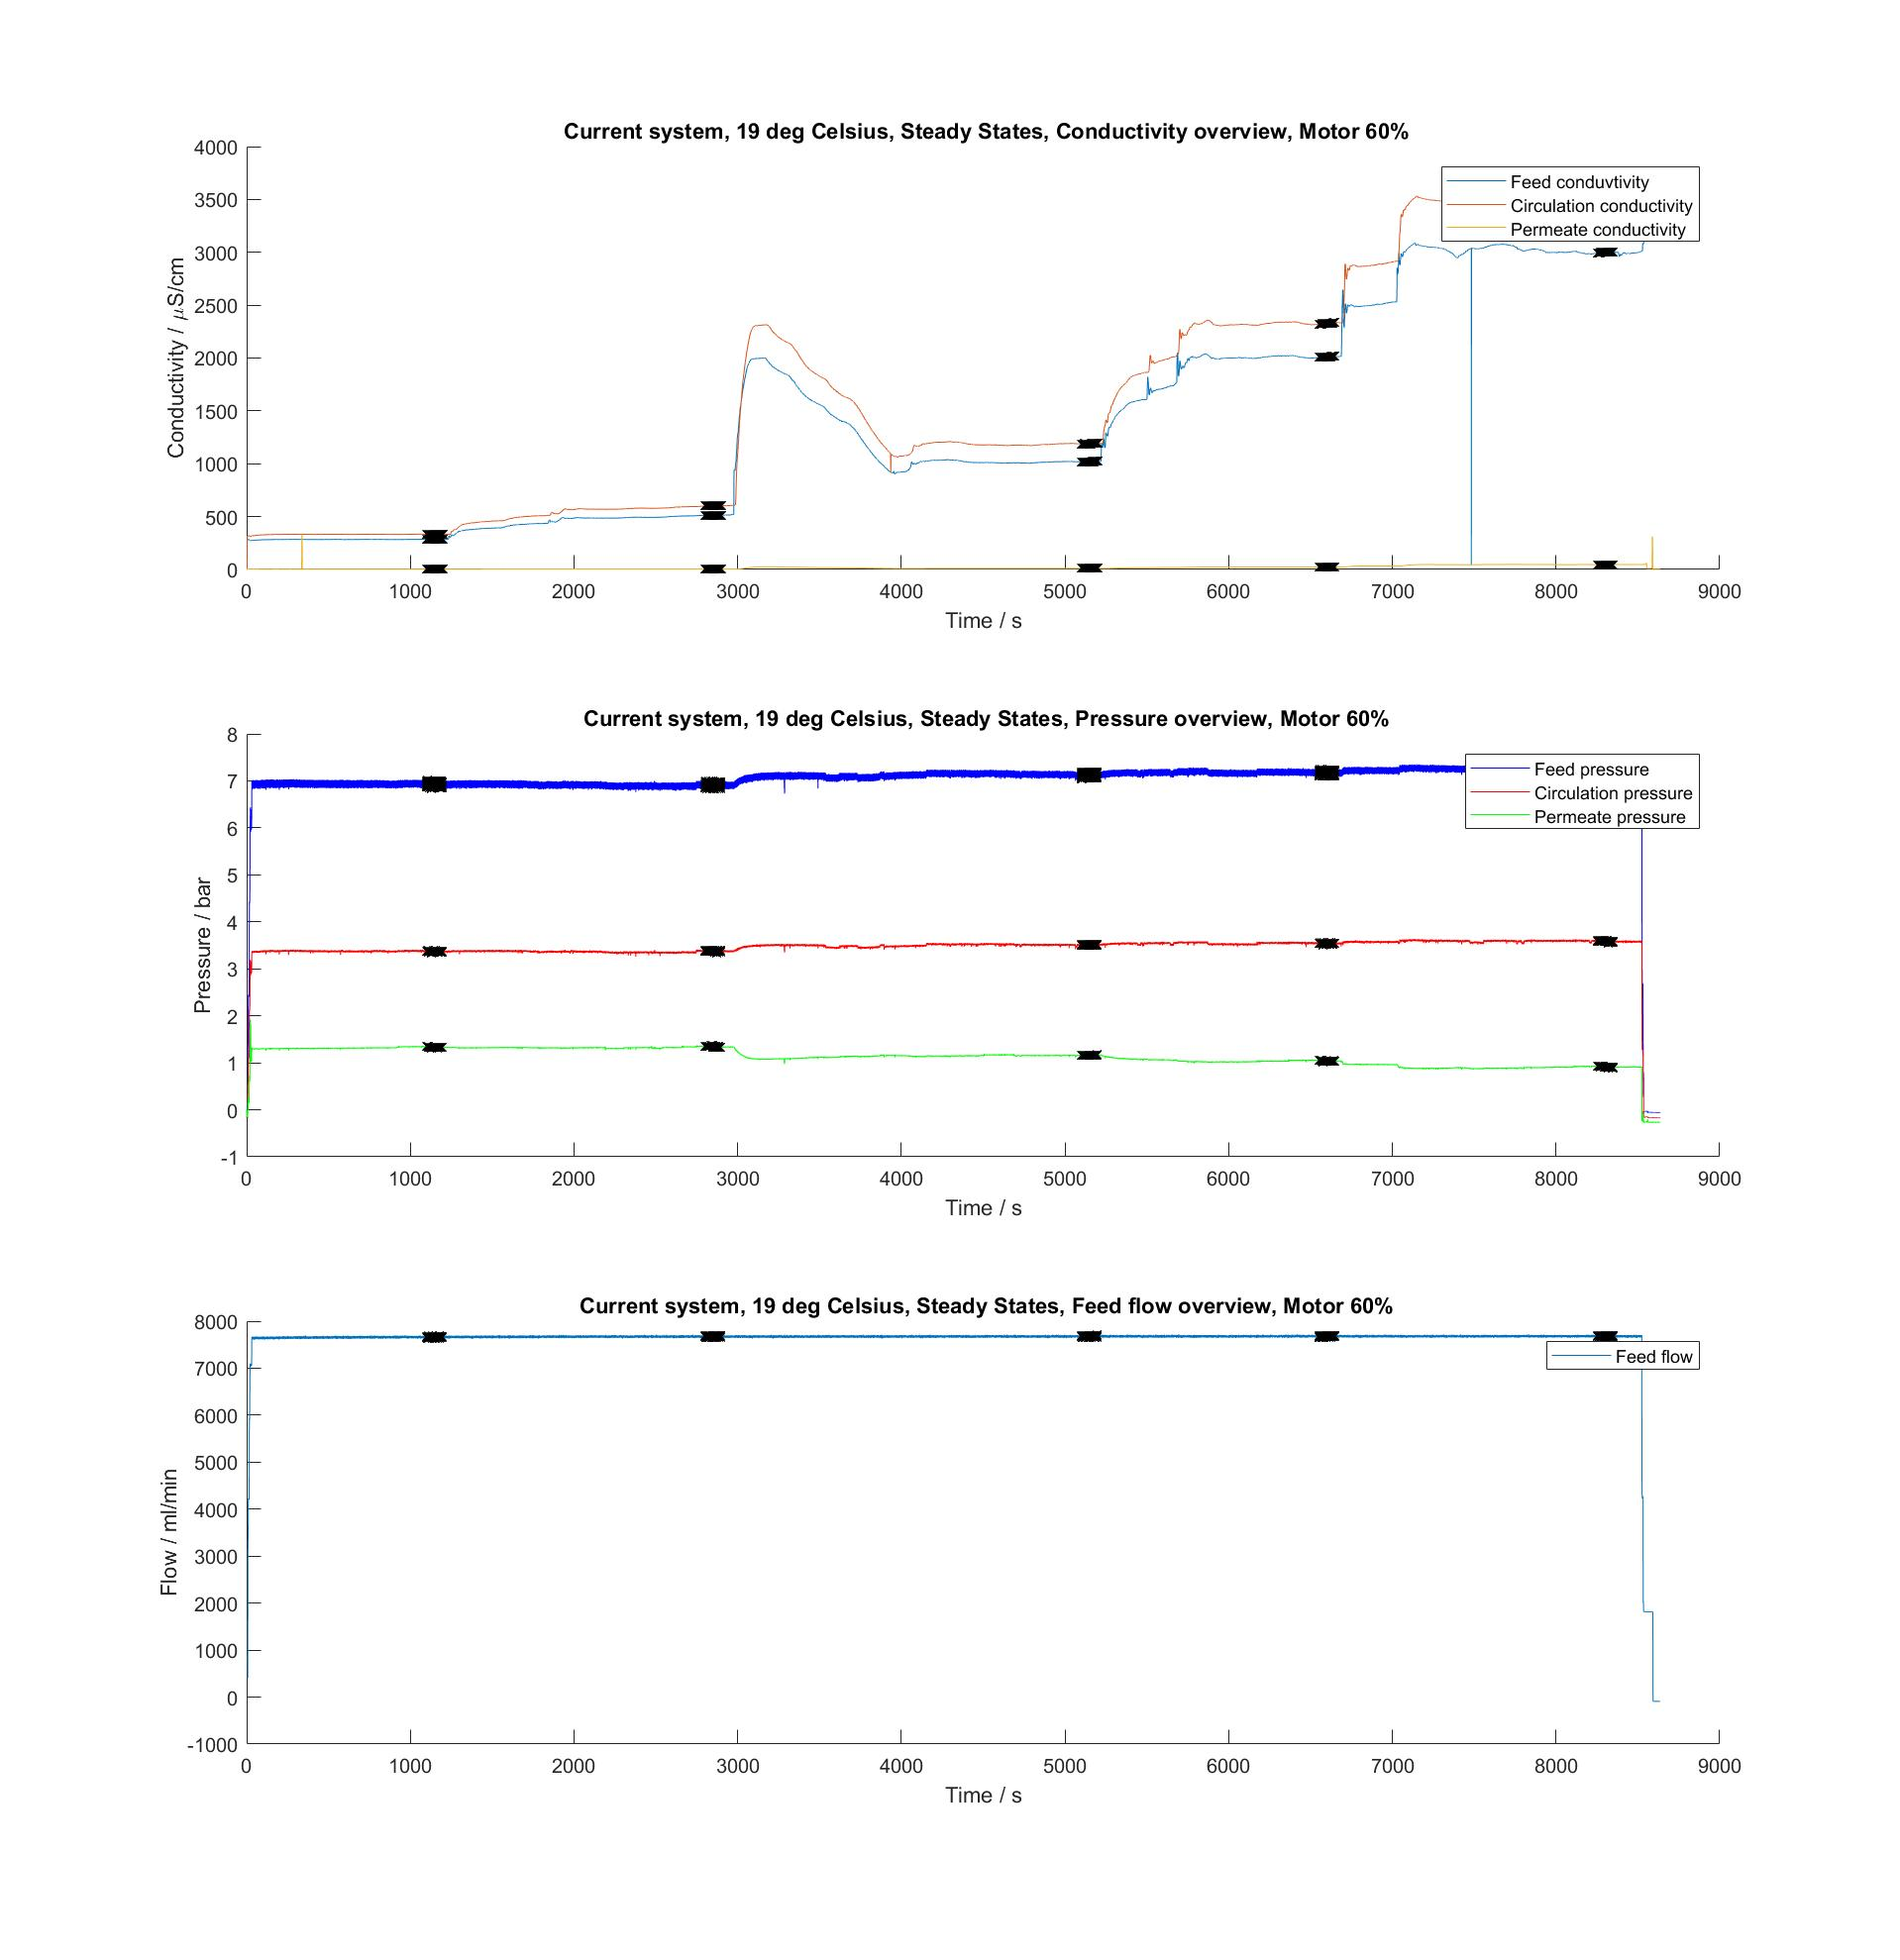
\includegraphics[width=1\textwidth]{overview20_60}
    \caption{Test 1, Current system, 20 $^{\circ}$C. Steady states 1.1, 1.2, 1.3, 1.5 and 1.7 }
    \label{fig:SteadyStates20C_1}
\end{figure}

\newpage

\subsection{Current system, Test sequence 1, part 2}
  
\begin{figure}[H]
    \centering
    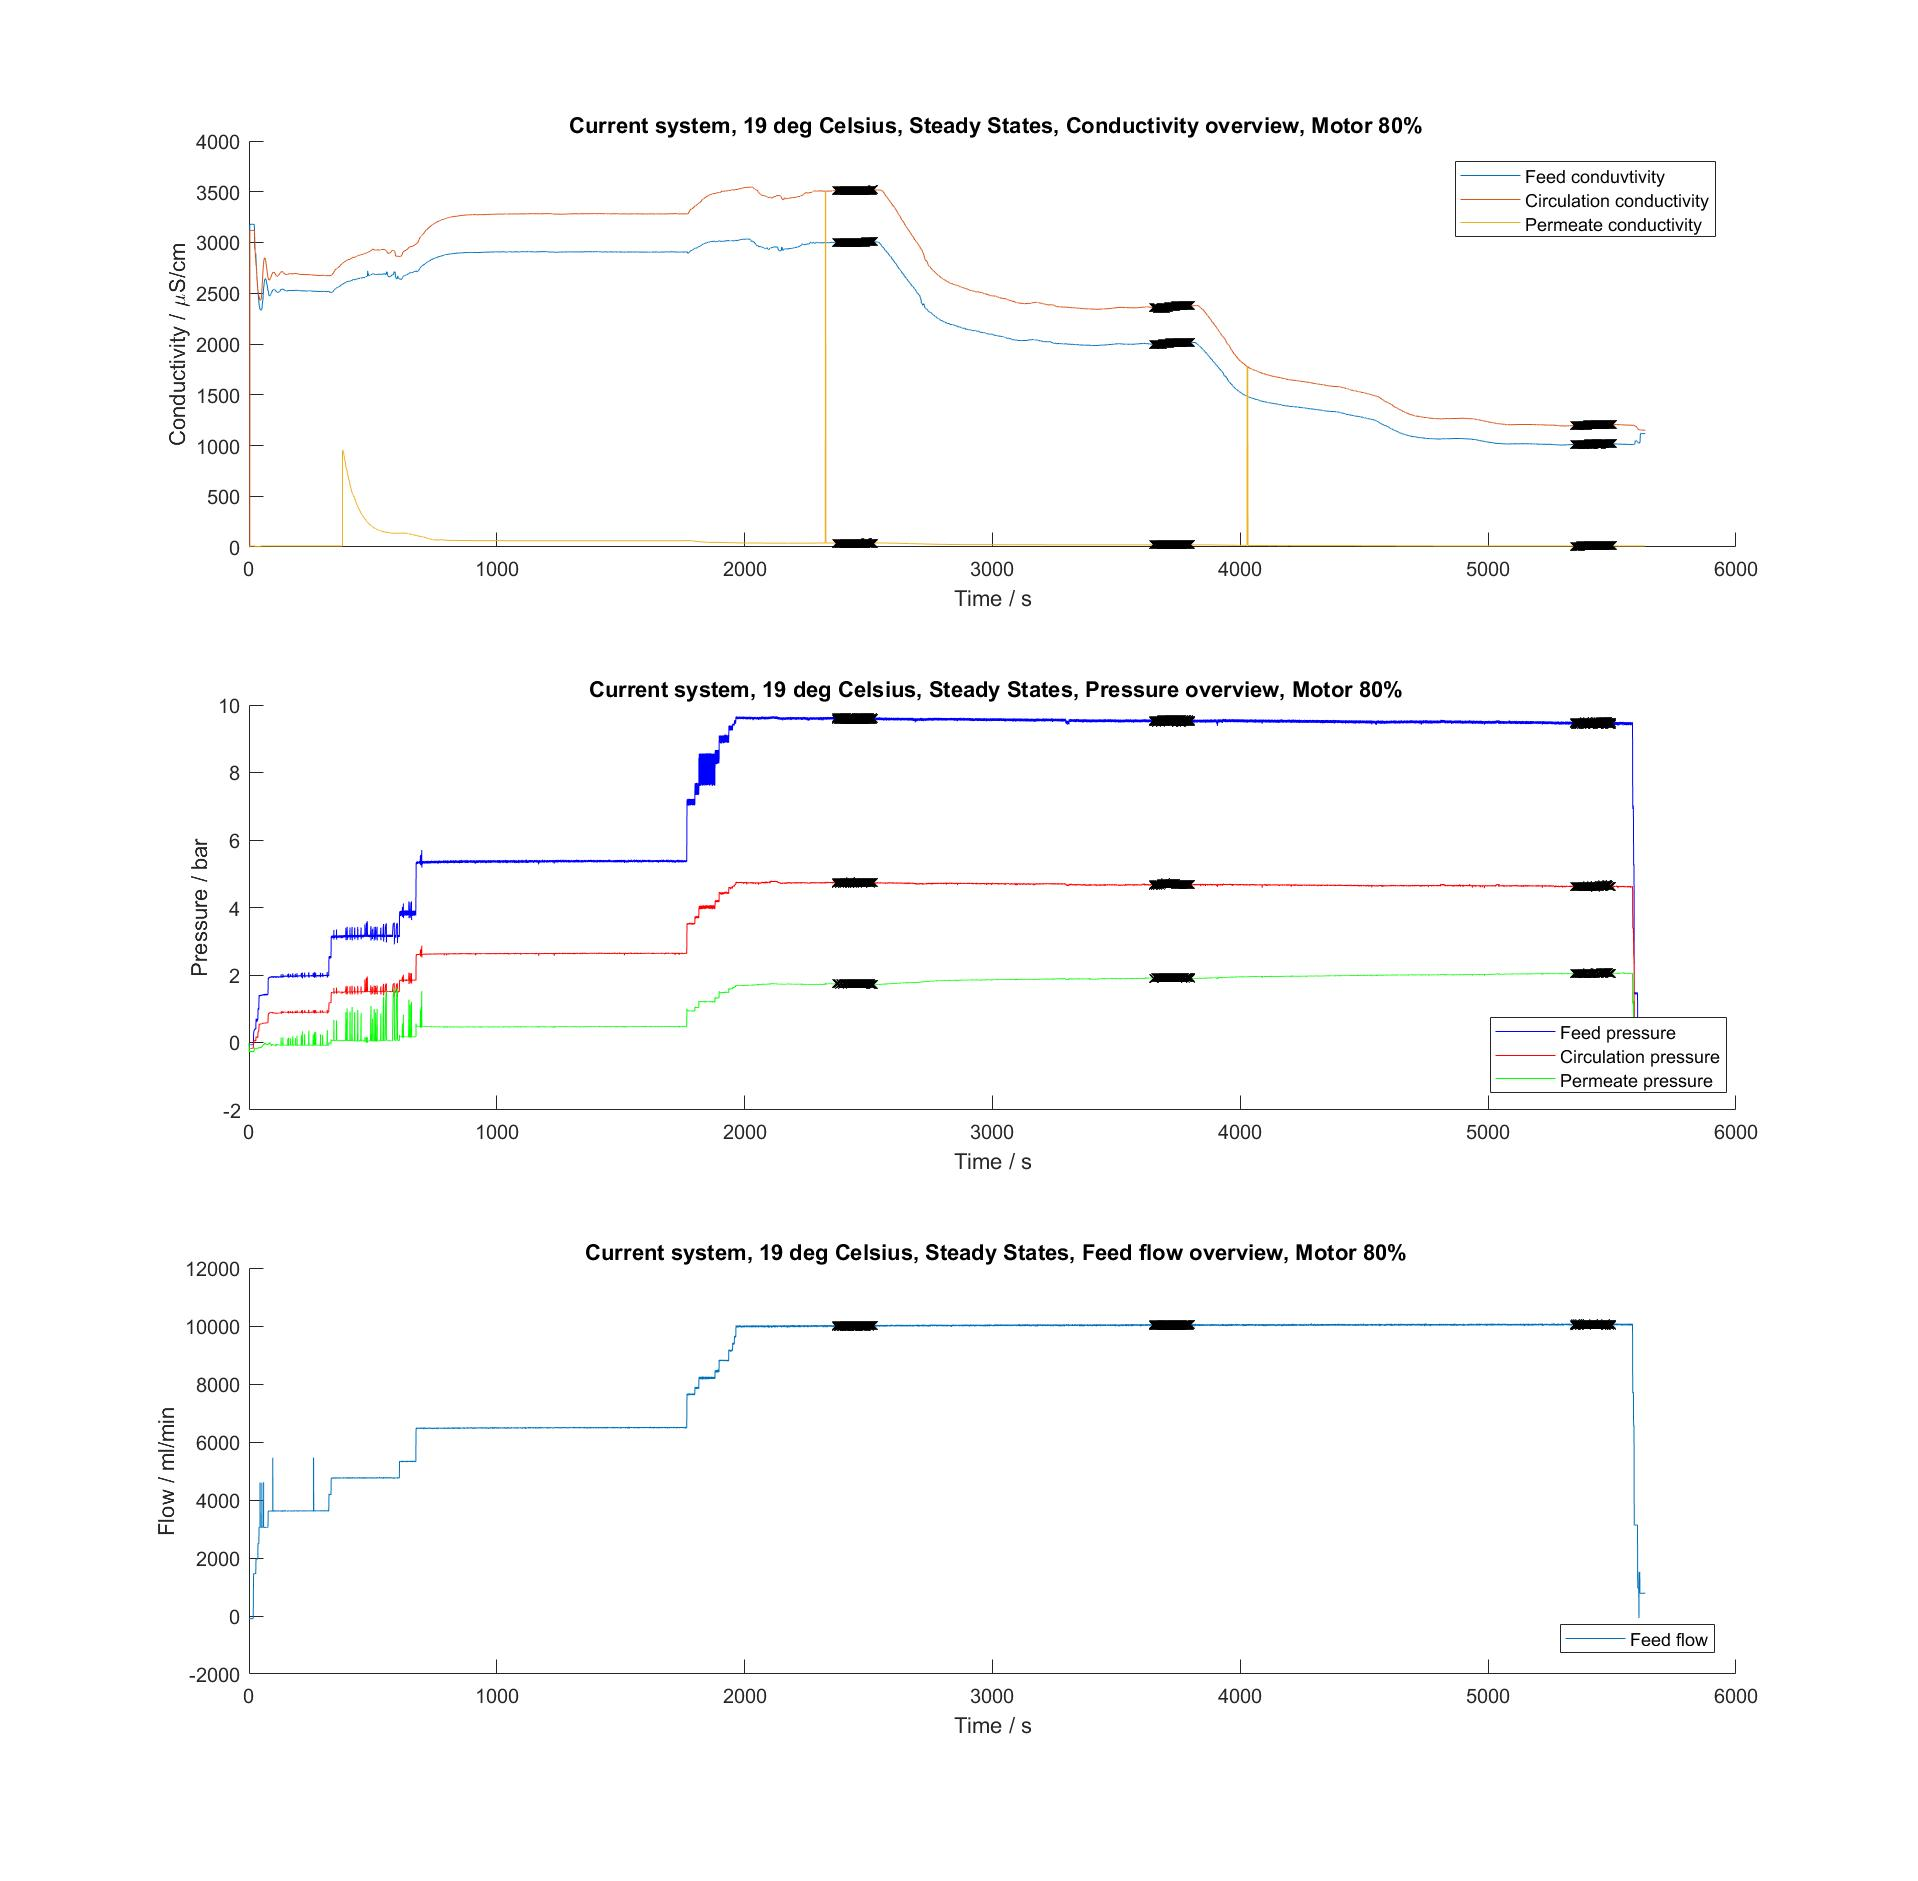
\includegraphics[width=1\textwidth]{overview20_80}
    \caption{Test 1, Current system, 20 $^{\circ}$C. Steady states 1.4, 1.6 and 1.8}
    \label{fig:SteadyStates20C_2}
\end{figure}

\newpage

By post-proccesing the data collected at the different steady states in test sequence 1 in Matlab it was possible to visually show how the system parameters were affected by the changed pump speed and feed conductivity. The results can be seen in figure \ref{fig:K20}.  


\begin{figure}[H]
    \centering
    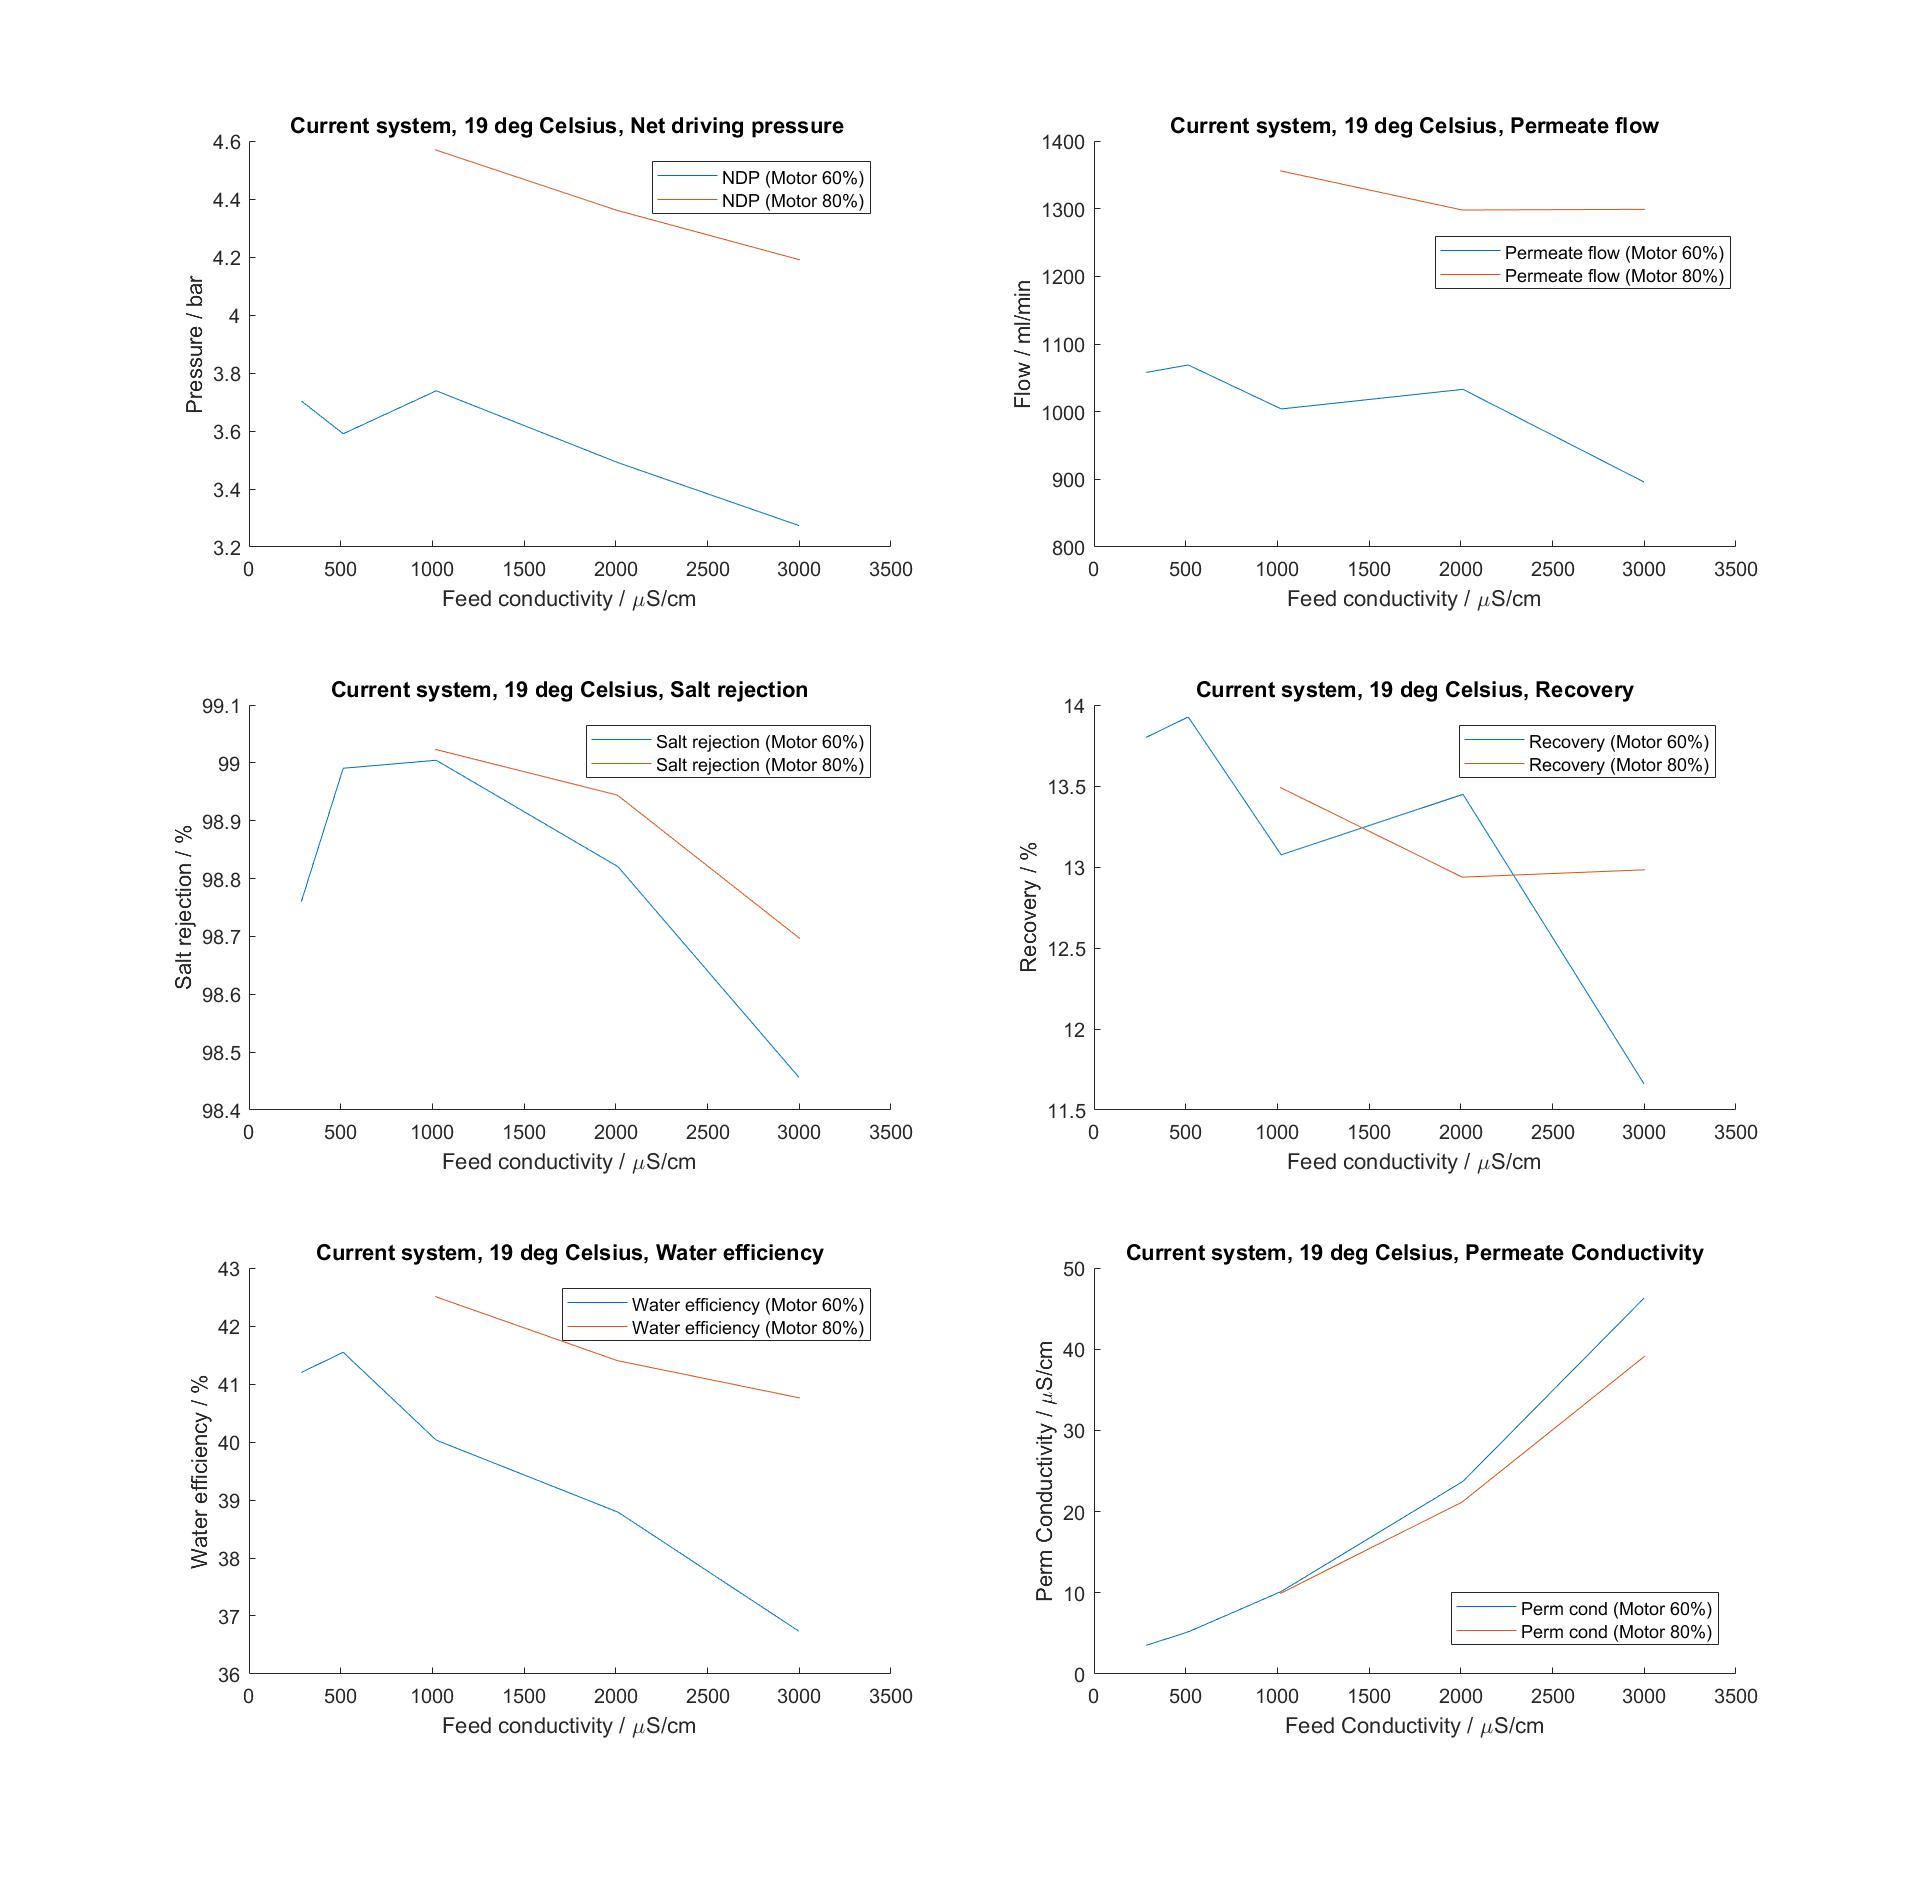
\includegraphics[width=1\textwidth]{Key20}
    \caption{Graphs containing information on how the system performed during test sequence 1. The values used in the plots were calculated from the steady state measurements and show how the system changed when the feed conductivity, feed pump RPM was increased.}
    \label{fig:K20}
\end{figure}

\newpage

\subsection{Current system, Test sequence 2}

The second test was carried out by setting the heater bath to 30 $^{\circ}$C and and adjusting the conductivity and pump speed according to the test plan. Since the water was much warmer than the air in the room, the heating caused by the pump was not as prominent and allowed all steady states to be examined in one continuous test. 

\begin{figure}[H]
    \centering
    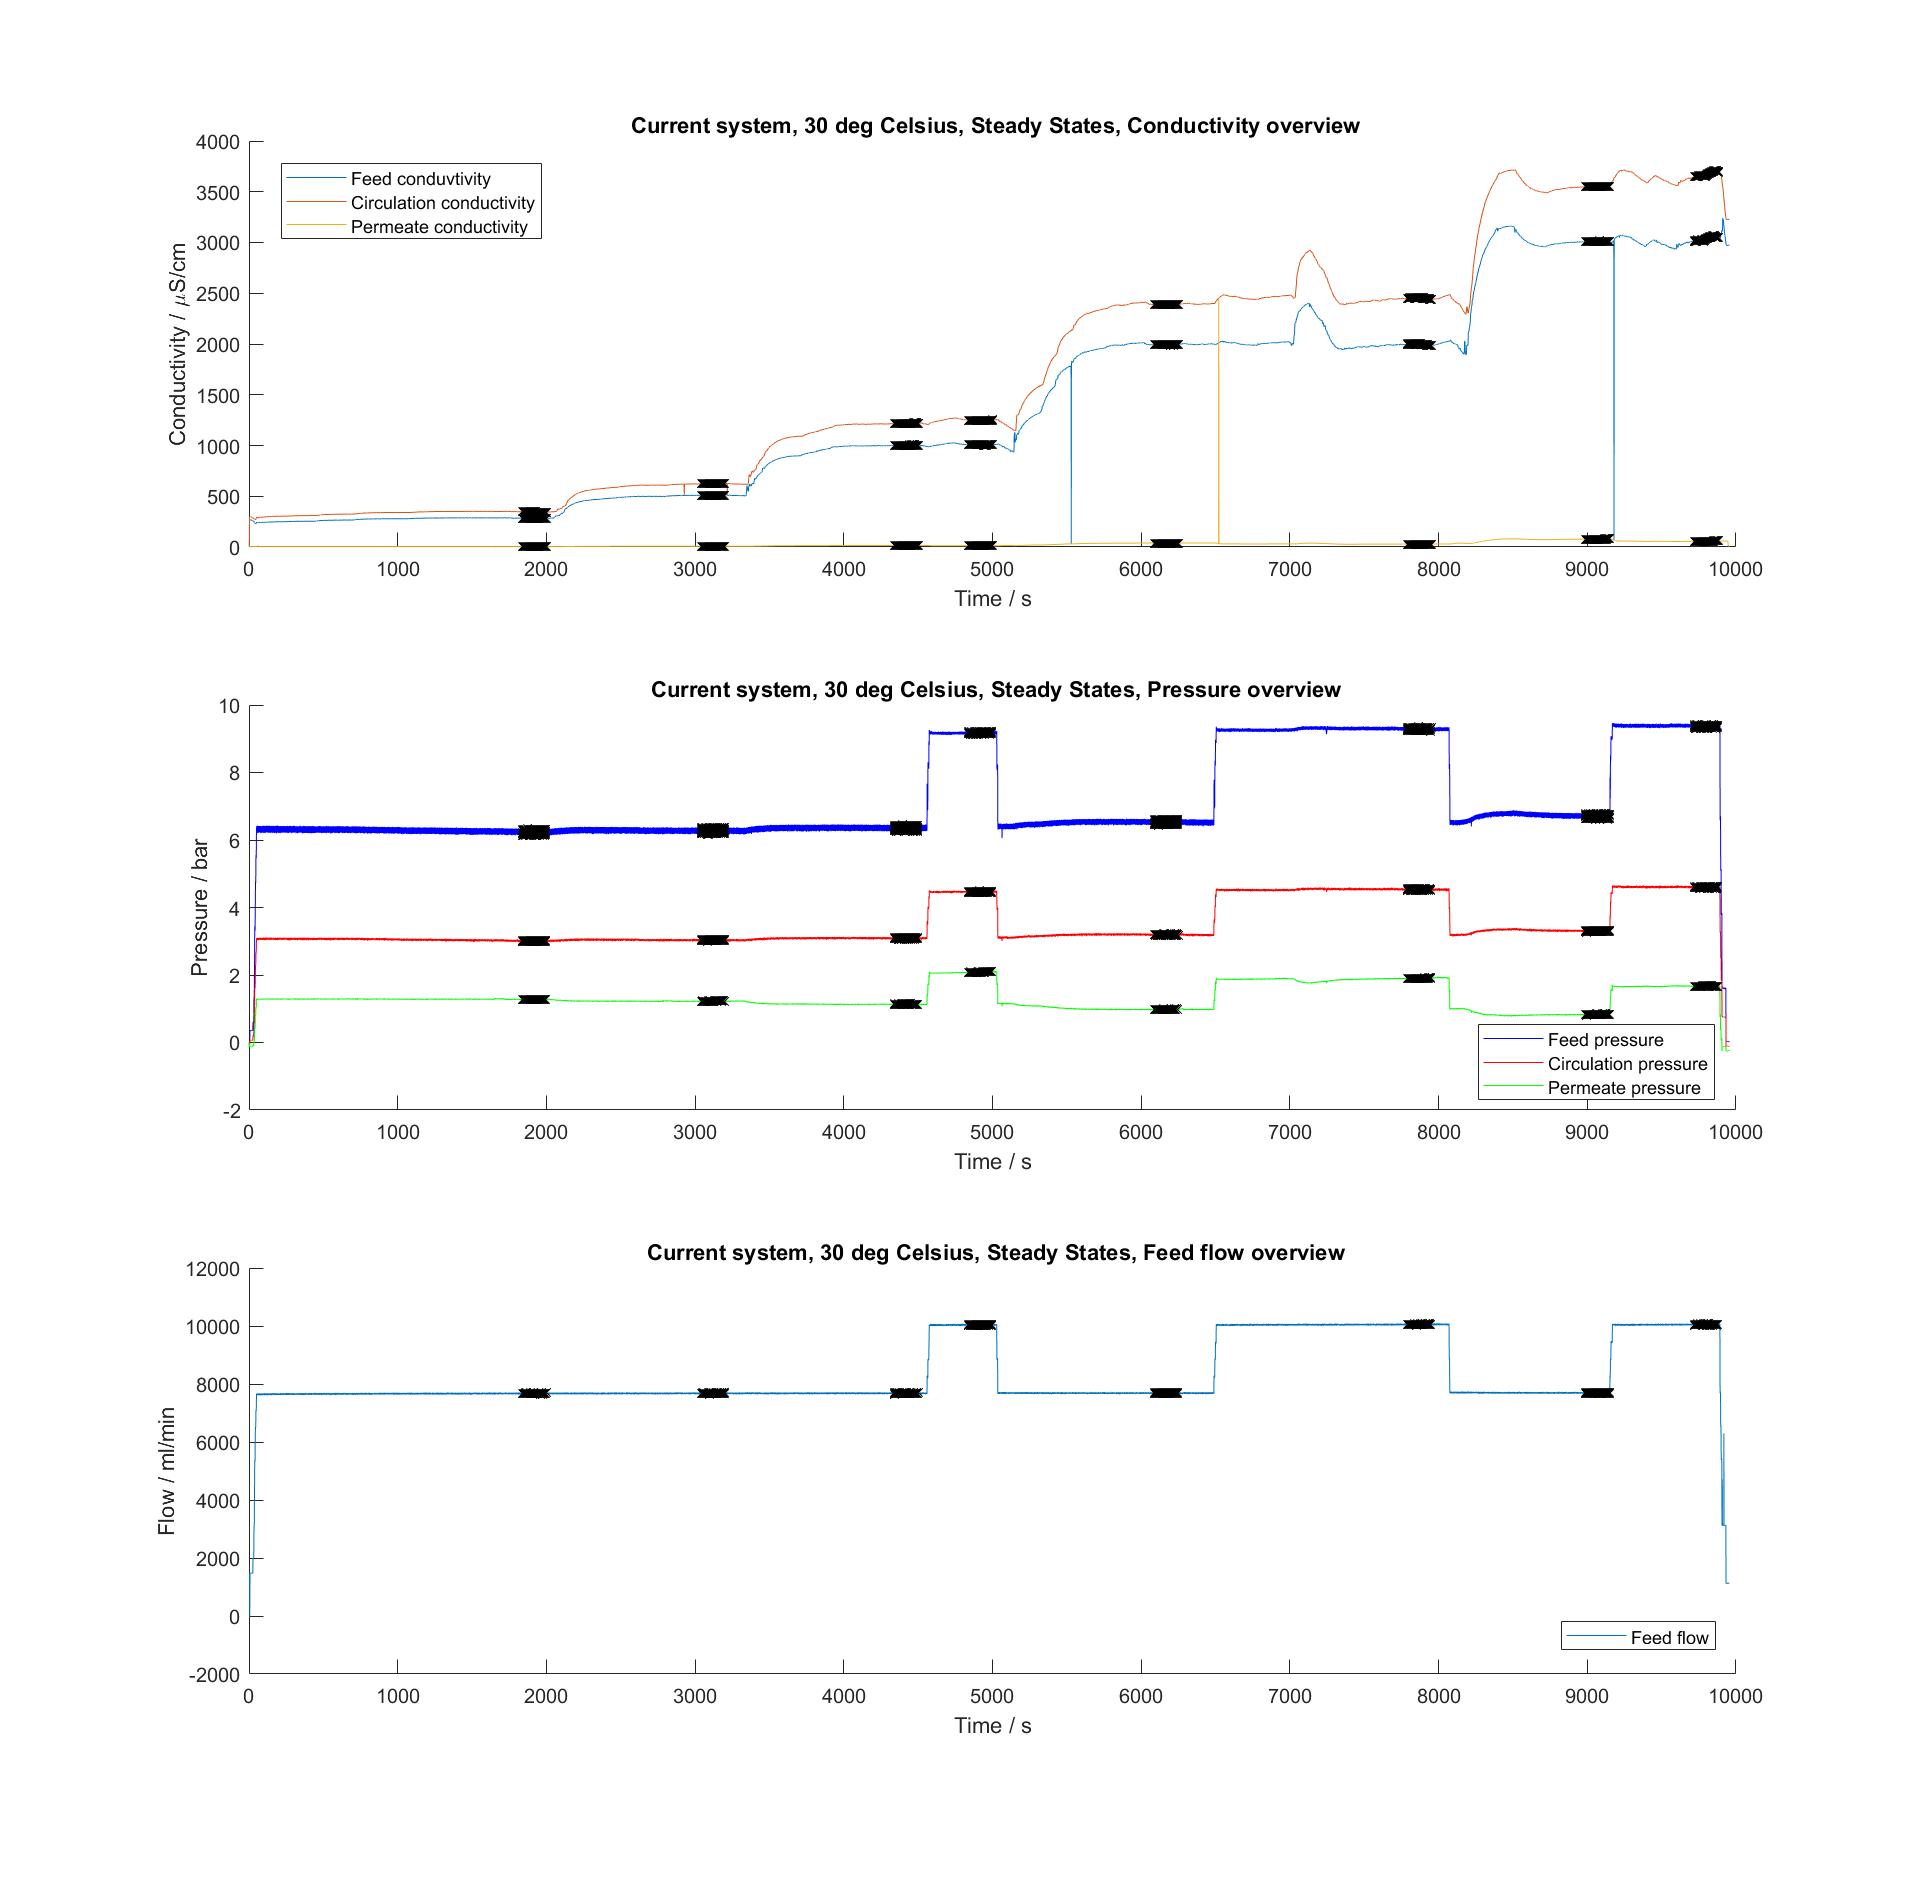
\includegraphics[width=1.1\textwidth]{overview30}
    \caption{Test 2, Current system, 30 $^{\circ}$C. Steady states 2.1, 2.2, 2.3, 2.4 2.5, 2.6, 2.7 and 2.8}
    \label{fig:overw30}
\end{figure}

\newpage


The data from the test was post processed in Matlab in exactly the same way as the previous test. The results are displayed in figure \ref{fig:K30}. 

\begin{figure}[H]
    \centering
    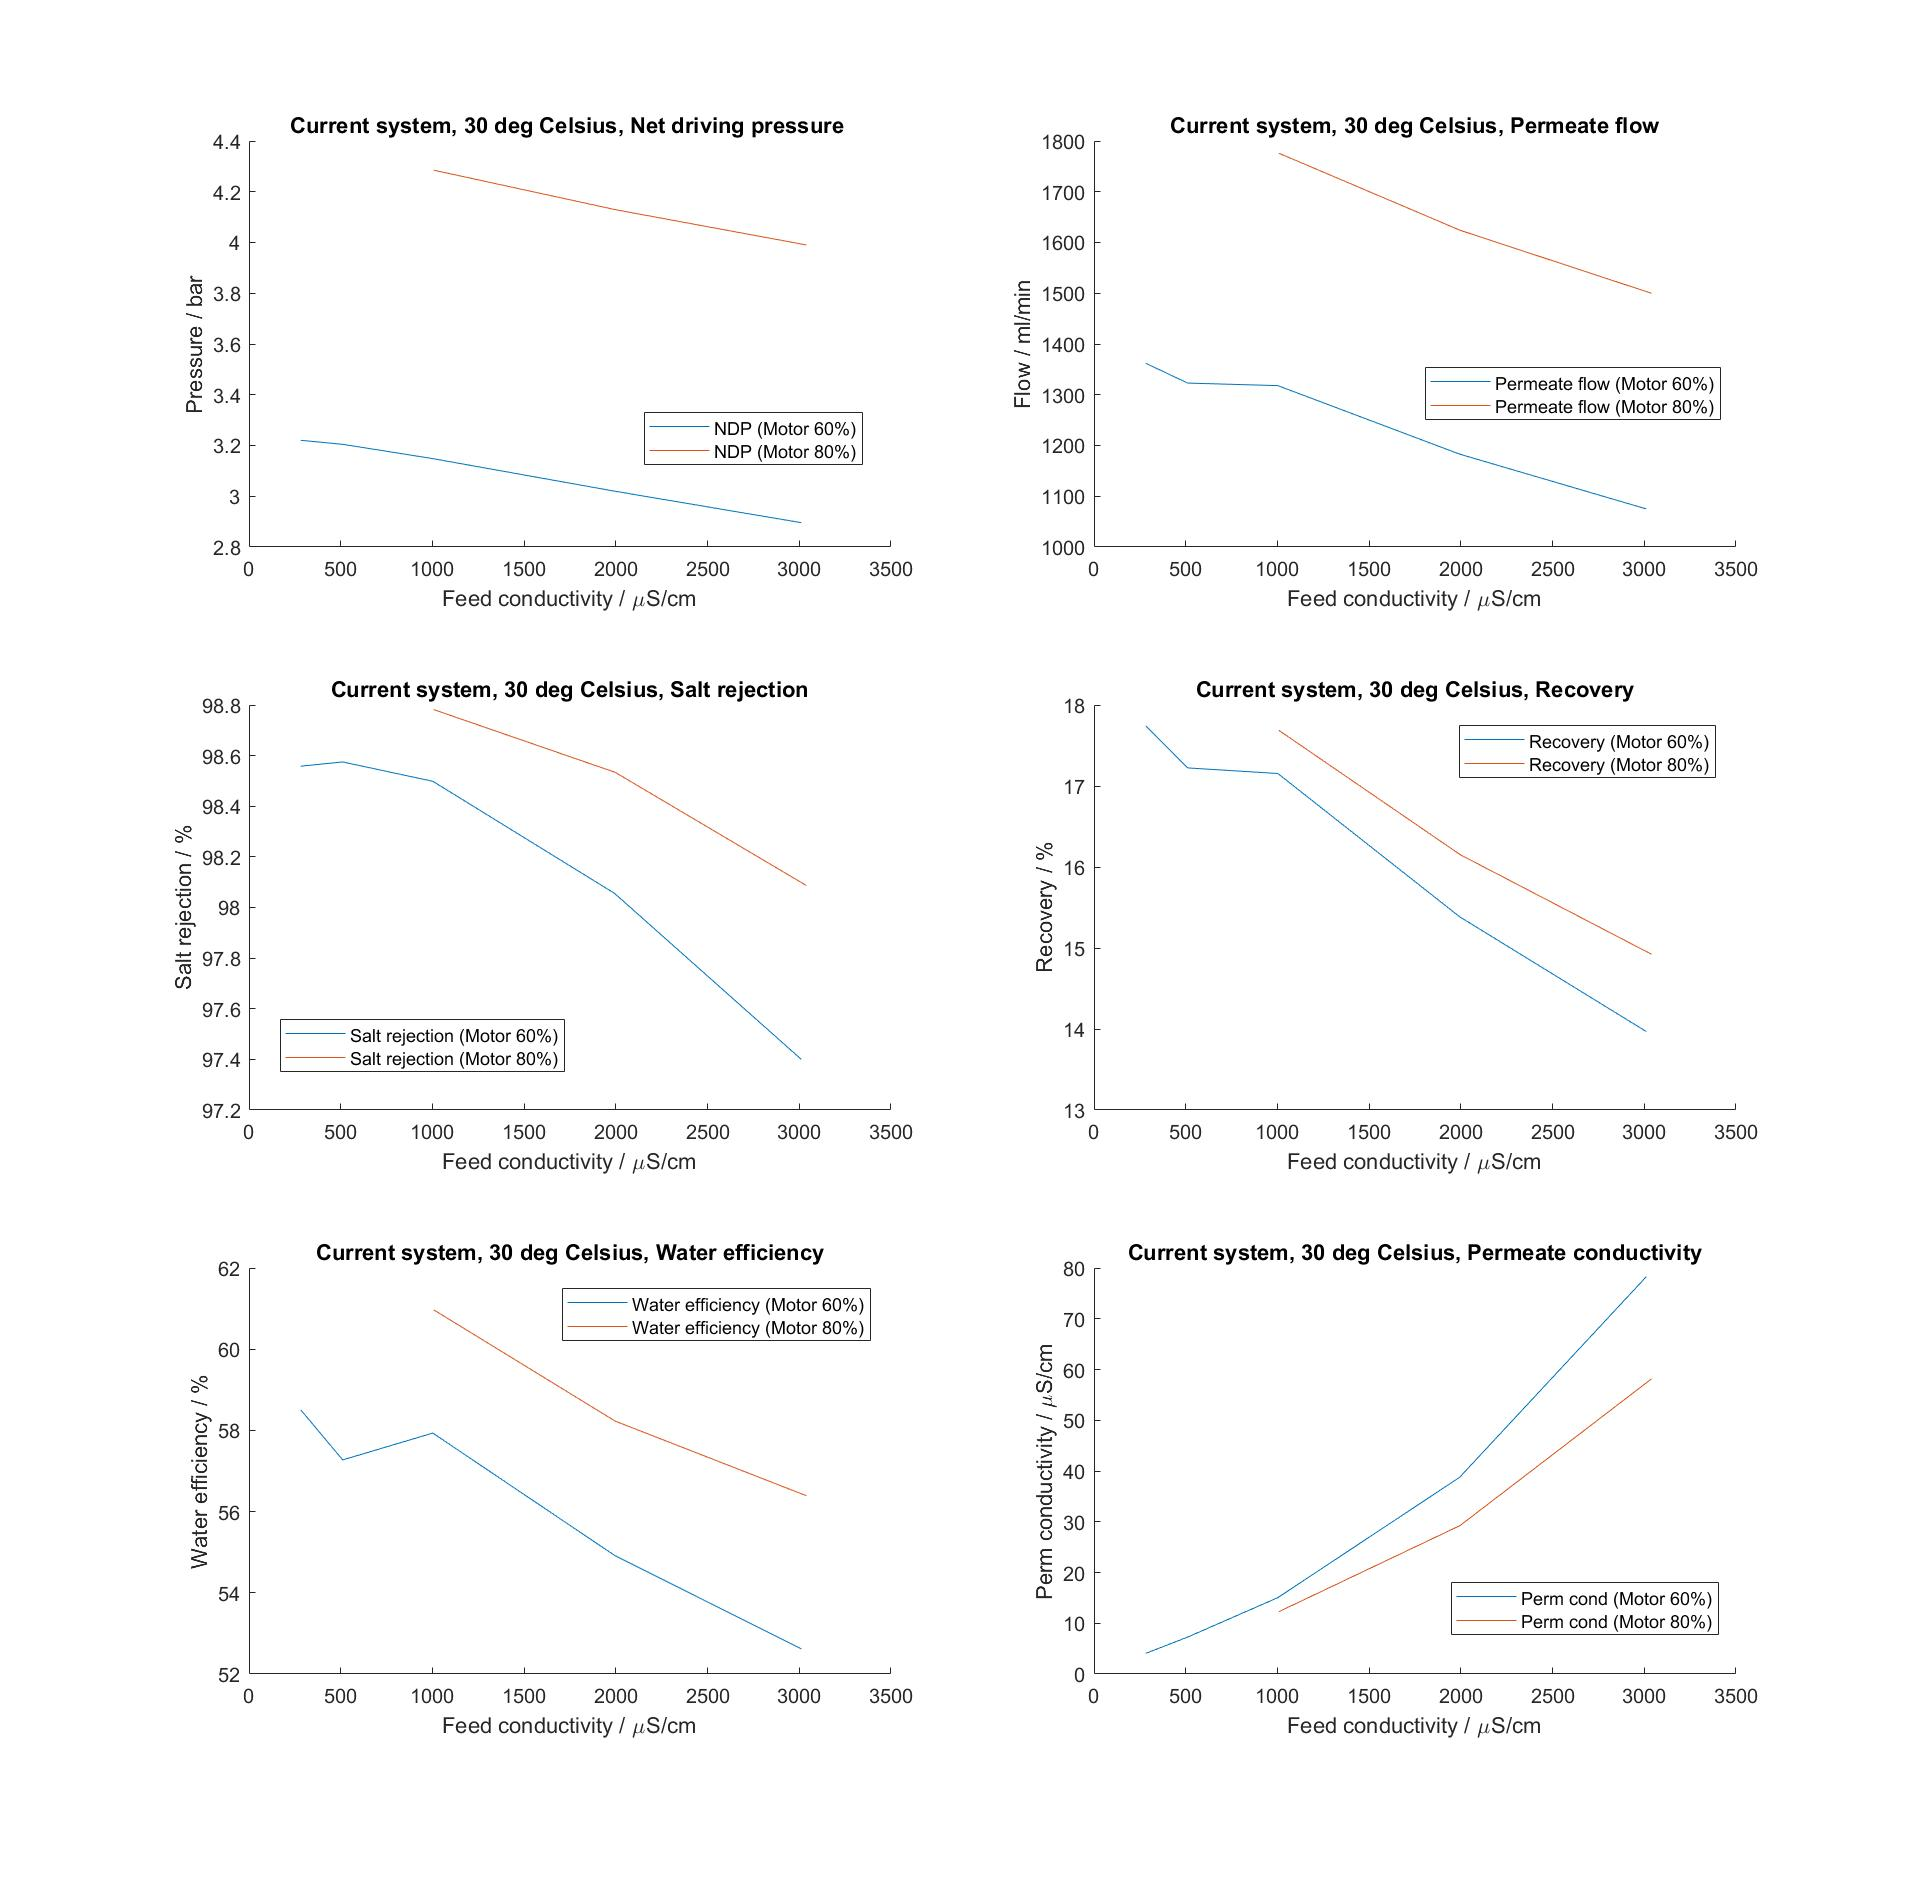
\includegraphics[width=1.1\textwidth]{Key30}
    \caption{Graphs containing information on how the system performed during test sequence 2. The values used in the plots were calculated from the steady state measurements and show how the system changed when the feed conductivity, feed pump RPM was increased.}
    \label{fig:K30}
\end{figure}

\newpage

\subsection{Current system, Test sequence 3}

Finally the heating bath was set to 40 $^{\circ}$C and the test sequence was performed just like test sequence 2. 

\begin{figure}[H]
    \centering
    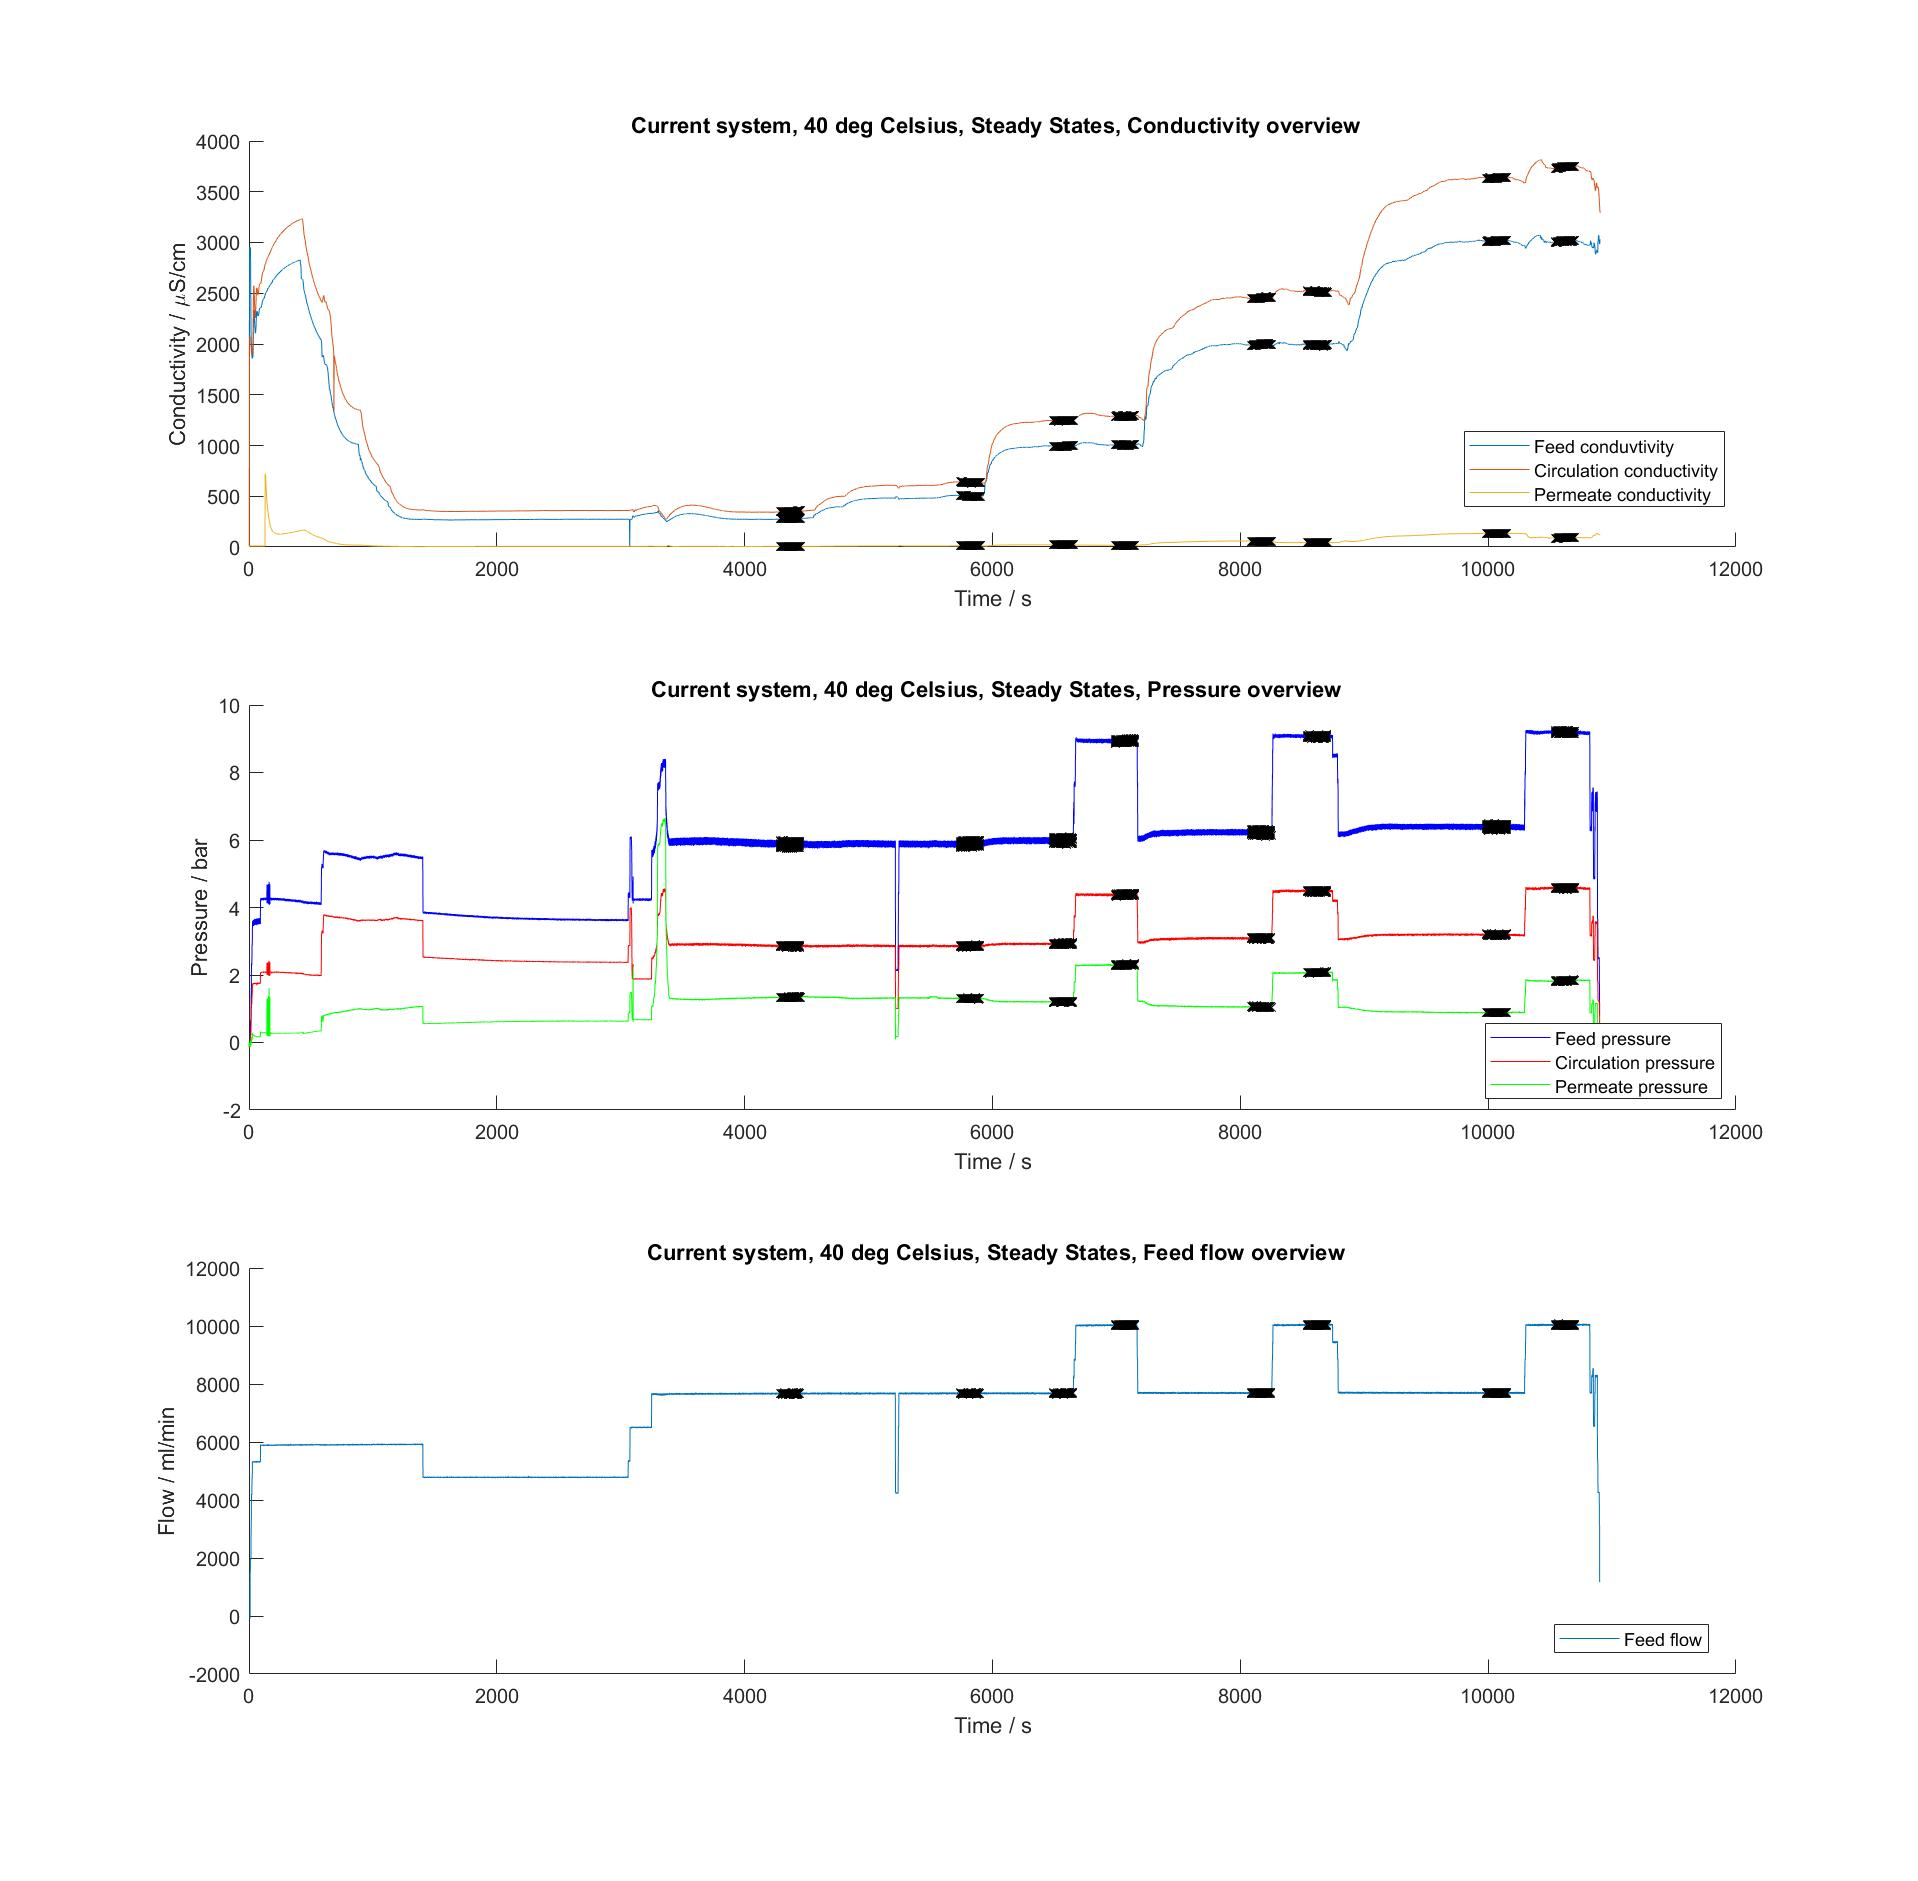
\includegraphics[width=1.1\textwidth]{overview40}
    \caption{Test 3, Current system, 30 $^{\circ}$C. Steady states 3.1, 3.2, 3.3, 3.4 3.5, 3.6, 3.7 and 3.8}
    \label{fig:overw40}
\end{figure}

\newpage

Post processing in Matlab generated the following data from the steady states.

\begin{figure}[H]
    \centering
    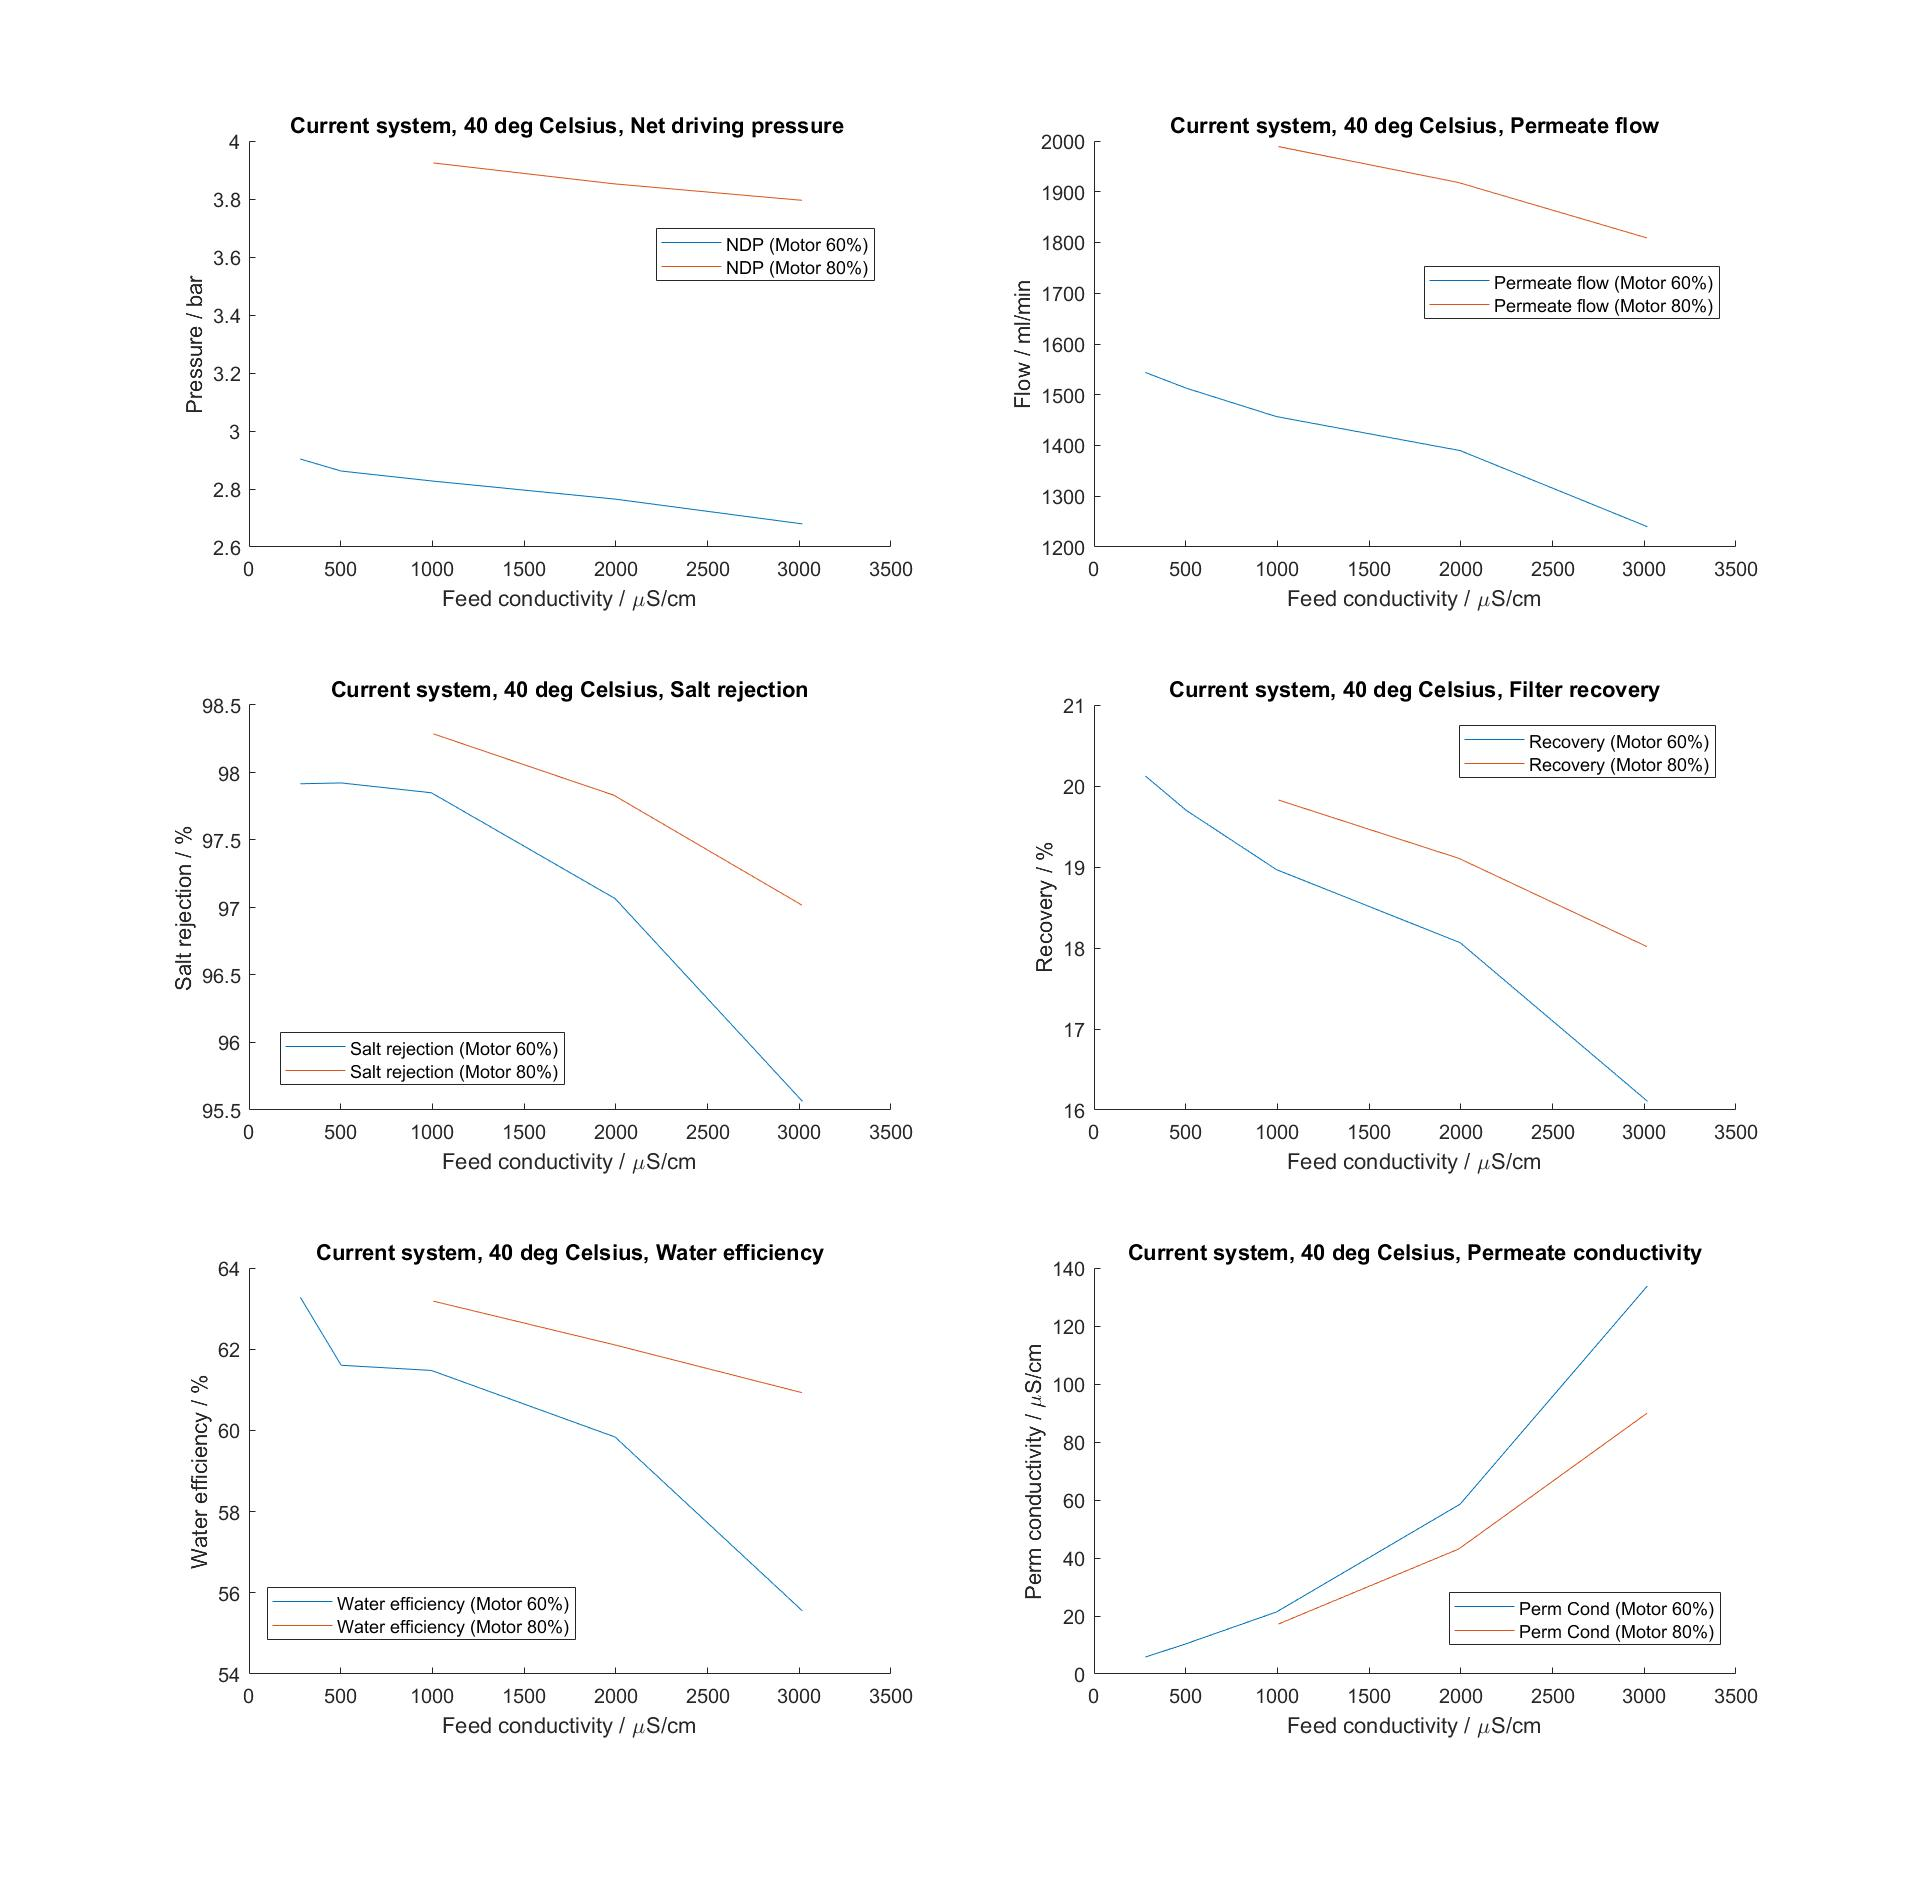
\includegraphics[width=1.1\textwidth]{Key40}
    \caption{Graphs containing information on how the system performed during test sequence 3. The values used in the plots were calculated from the steady state measurements and show how the system changed when the feed conductivity, feed pump RPM was increased.}
    \label{fig:K40}
\end{figure}

\newpage

In order to understand how the current system performed in different working conditions all plots from the post processing in Matlab were put togeheter. By doing this, it was possible to visualize the effect of temperature on the system parameters. The following plots explain in more detail how the system parameters changed when the system temperature, feed conductivity and feed pressure incresed.  

\subsection{Net driving pressure}

Net driving pressure was decreased when the temperature was increased. Higher feed conductivity resulted in a decreased net driving pressure. As expected, running the feed pump at a higher RPM also increased the net driving pressure.

\begin{figure}[H]
    \centering
    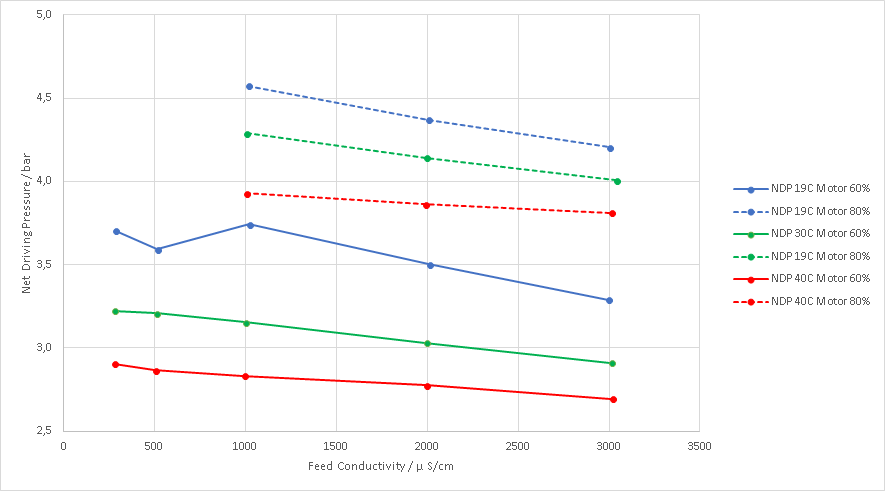
\includegraphics[width=0.8\textwidth]{NDP}
    \caption{Net Driving Pressure, NDP (Pressure difference from feed to permeate side of the membrane minus the osmotic pressure)}
    \label{fig:NDP}
\end{figure}

\subsection{Permeate flow}

According to theory, net driving pressure has a direct effect on permeate flow. When the feed pump was increased more water was pushed through the membrane. Increased water temperatures caused a higher permeate flow. For instance, the permeate flow increased by around 50\% when the temperature was increased from 20 $^{\circ}$C to 40 $^{\circ}$C and the pump was running at 60\%. Due to the increased osmotic pressure, permeate flow decreased when the feed conductivity increased

\begin{figure}[H]
    \centering
    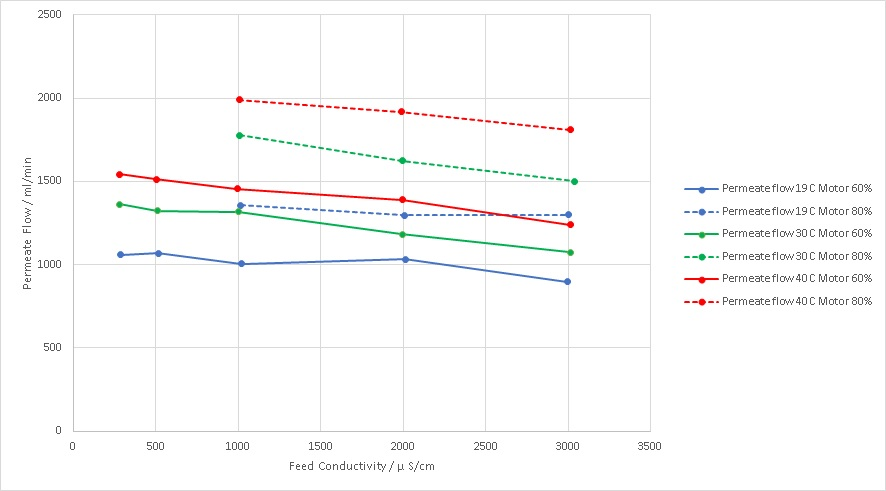
\includegraphics[width=0.8\textwidth]{permFlowCurrent}
    \caption{Permeate Flow (ml/min)}
    \label{fig:PermFC}
\end{figure}

\subsection{Recovery}

Warmer water enabled more feed water to pass through the membrane and therefore the recovery was increased. Increased conductivity reduced recovery due to the increased osmotic pressure.

\begin{figure}[H]
    \centering
    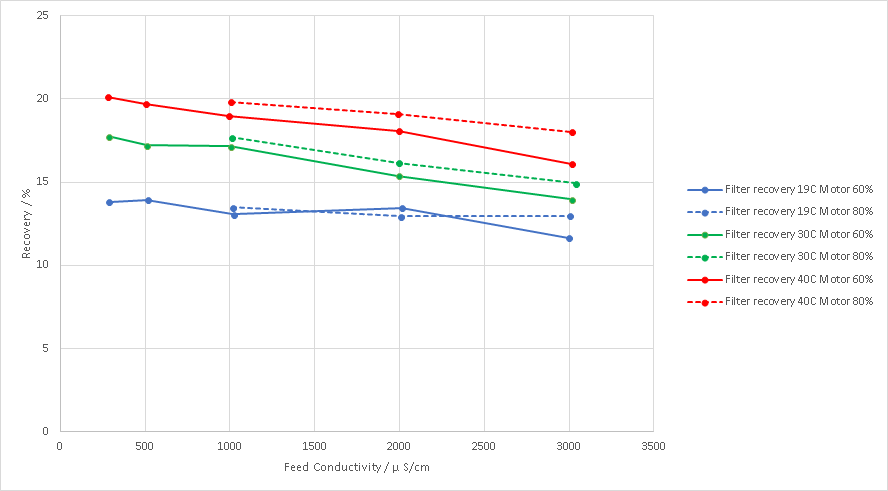
\includegraphics[width=0.8\textwidth]{Recovery}
    \caption{Recovery rate (\%)}
    \label{fig:rec}
\end{figure}

\subsection{Salt rejection}

By looking at figure \ref{fig:SaltRejectionResult} and \ref{fig:Permeatecond} the deterimental effects of both increased temperature and feed conductivity can be seen. The negative effect of increased feed conductivity was much more prominent at 40 $^{\circ}$C than 30 $^{\circ}$C, which means that the performance of the membrane decreased with higher temperature. Increased feed pump pressure resulted in better salt rejection and the positive effect of increased pump pressure was larger when the system was hotter. Temperature was the parameter that decreased salt rejection the most and by comparing how the system performed when the pump and feed conductivity was set to 60\% and 3000 \SI{}{\micro\siemens}/cm at 19 $^{\circ}$C and 40 $^{\circ}$C it can be seen that the salt rejection decreased from 98.5\% to 95.5 \%. From the experiment it can also be concluded that the system perform much better at low temperature and low feed conductivity than at high temperature and high feed conductivity. 

\begin{figure}[H]
    \centering
    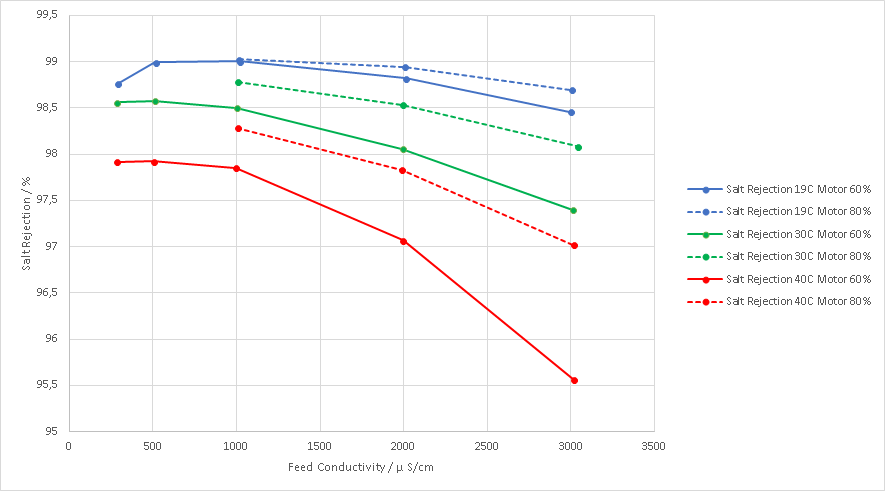
\includegraphics[width=0.8\textwidth]{SaltRejection}
    \caption{Salt Rejection (\%)}
    \label{fig:SaltRejectionResult}
\end{figure}
 
\subsection{Permeate conductivity}

Permeate conductivity was directly proportional to salt rejection at a certain temperature and feed conductivity. The black line in figure \ref{fig:Permeatecond} show the critical permeate conductivity that the system should be able to maintain and from the plot it is possible to se how high the feed conductivity can be without exceeding this limit.

\begin{figure}[H]
    \centering
    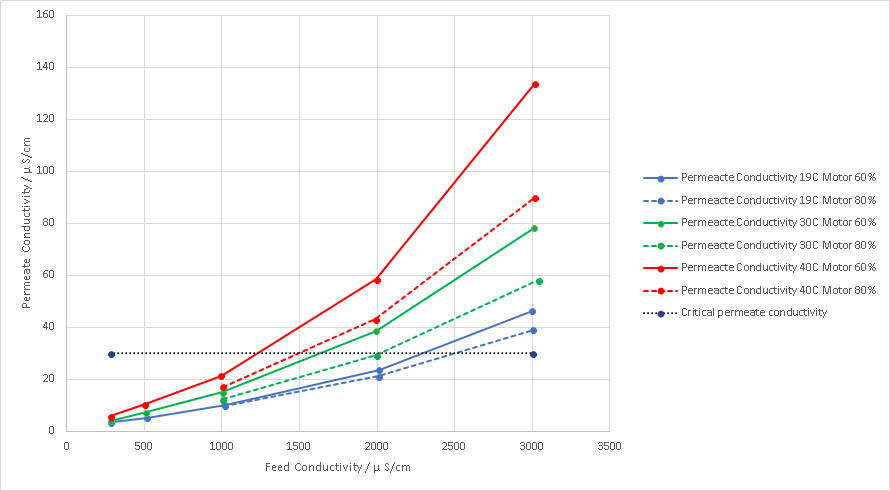
\includegraphics[width=0.8\textwidth]{PermCond}
    \caption{Permeate conductivity (\SI{}{\micro\siemens}/cm)}
    \label{fig:Permeatecond}
\end{figure}


\subsection{Water efficiency}

Water efficiency increased when the temperature increased due to more permeate water being generated by the same feed pressure. Increased feed pressure also increased water efficiency. 

\begin{figure}[H]
    \centering
    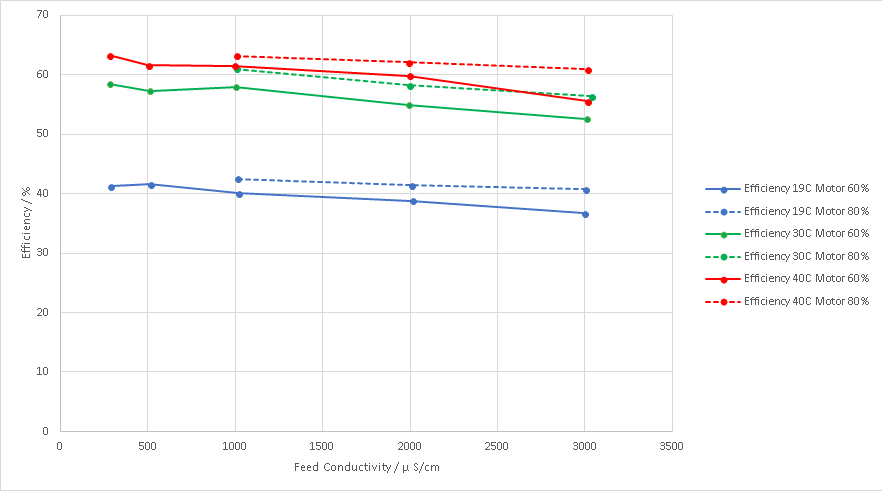
\includegraphics[width=0.8\textwidth]{Efficiency}
    \caption{Water Efficiency}
    \label{fig:Weff}
\end{figure}

\newpage

\subsection{System 2}

The circulation pump, a motorized drain valve and a flow meter on the permeate side was added to the system and the flow path was modified according to figure \ref{fig:System2_1}. The rig was also reprogrammed to be able to measure all flows in the flow path in real time. This could be done because now both the feed flow, circulation flow and permeate flow could be measured and from this data, the inlet and drain flow could be calculated.  

\begin{figure}[H]
  \centering
  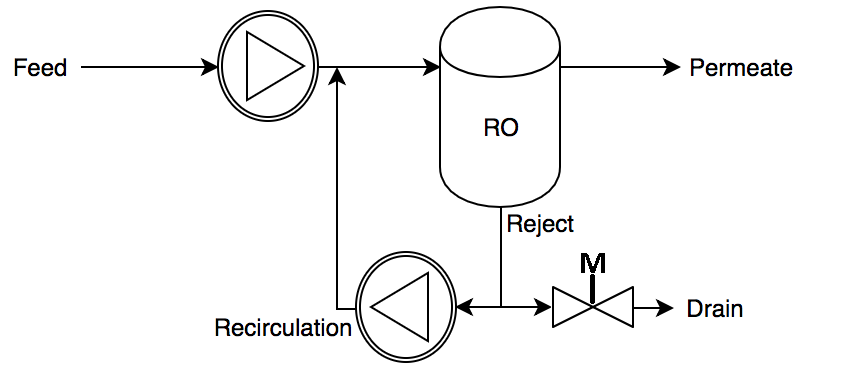
\includegraphics[width=1\linewidth]{Sys2}
  \caption{Two pump system, with one pump on feed side and one pump in the recirculation loop}
  \label{fig:System2_1}
\end{figure}


\newpage
\subsubsection{Increased circulation}

The Initial idea for optimising the membrane was to use the circulation pump to create a turbulent flow close to the membrane surface. Therefore, a test was set up to test this idea.
During the test, the feed pump and drain valve was set to a fixed value and the circulation pump was increased from 5\% to 35\%. Figure \ref{fig:RecIncrease40} shows the permeate conductivity, circulation flow and feed pressure and 7 steady state points from the test.\\
\\
The circulation flow was increased from 1500 ml/min to 5000 ml/min and the increased circulation flow caused the pressure to increase from 5.5 to 7 bar. The permeate conductivity remained unchanged. 
\begin{figure}[H]
    \centering
    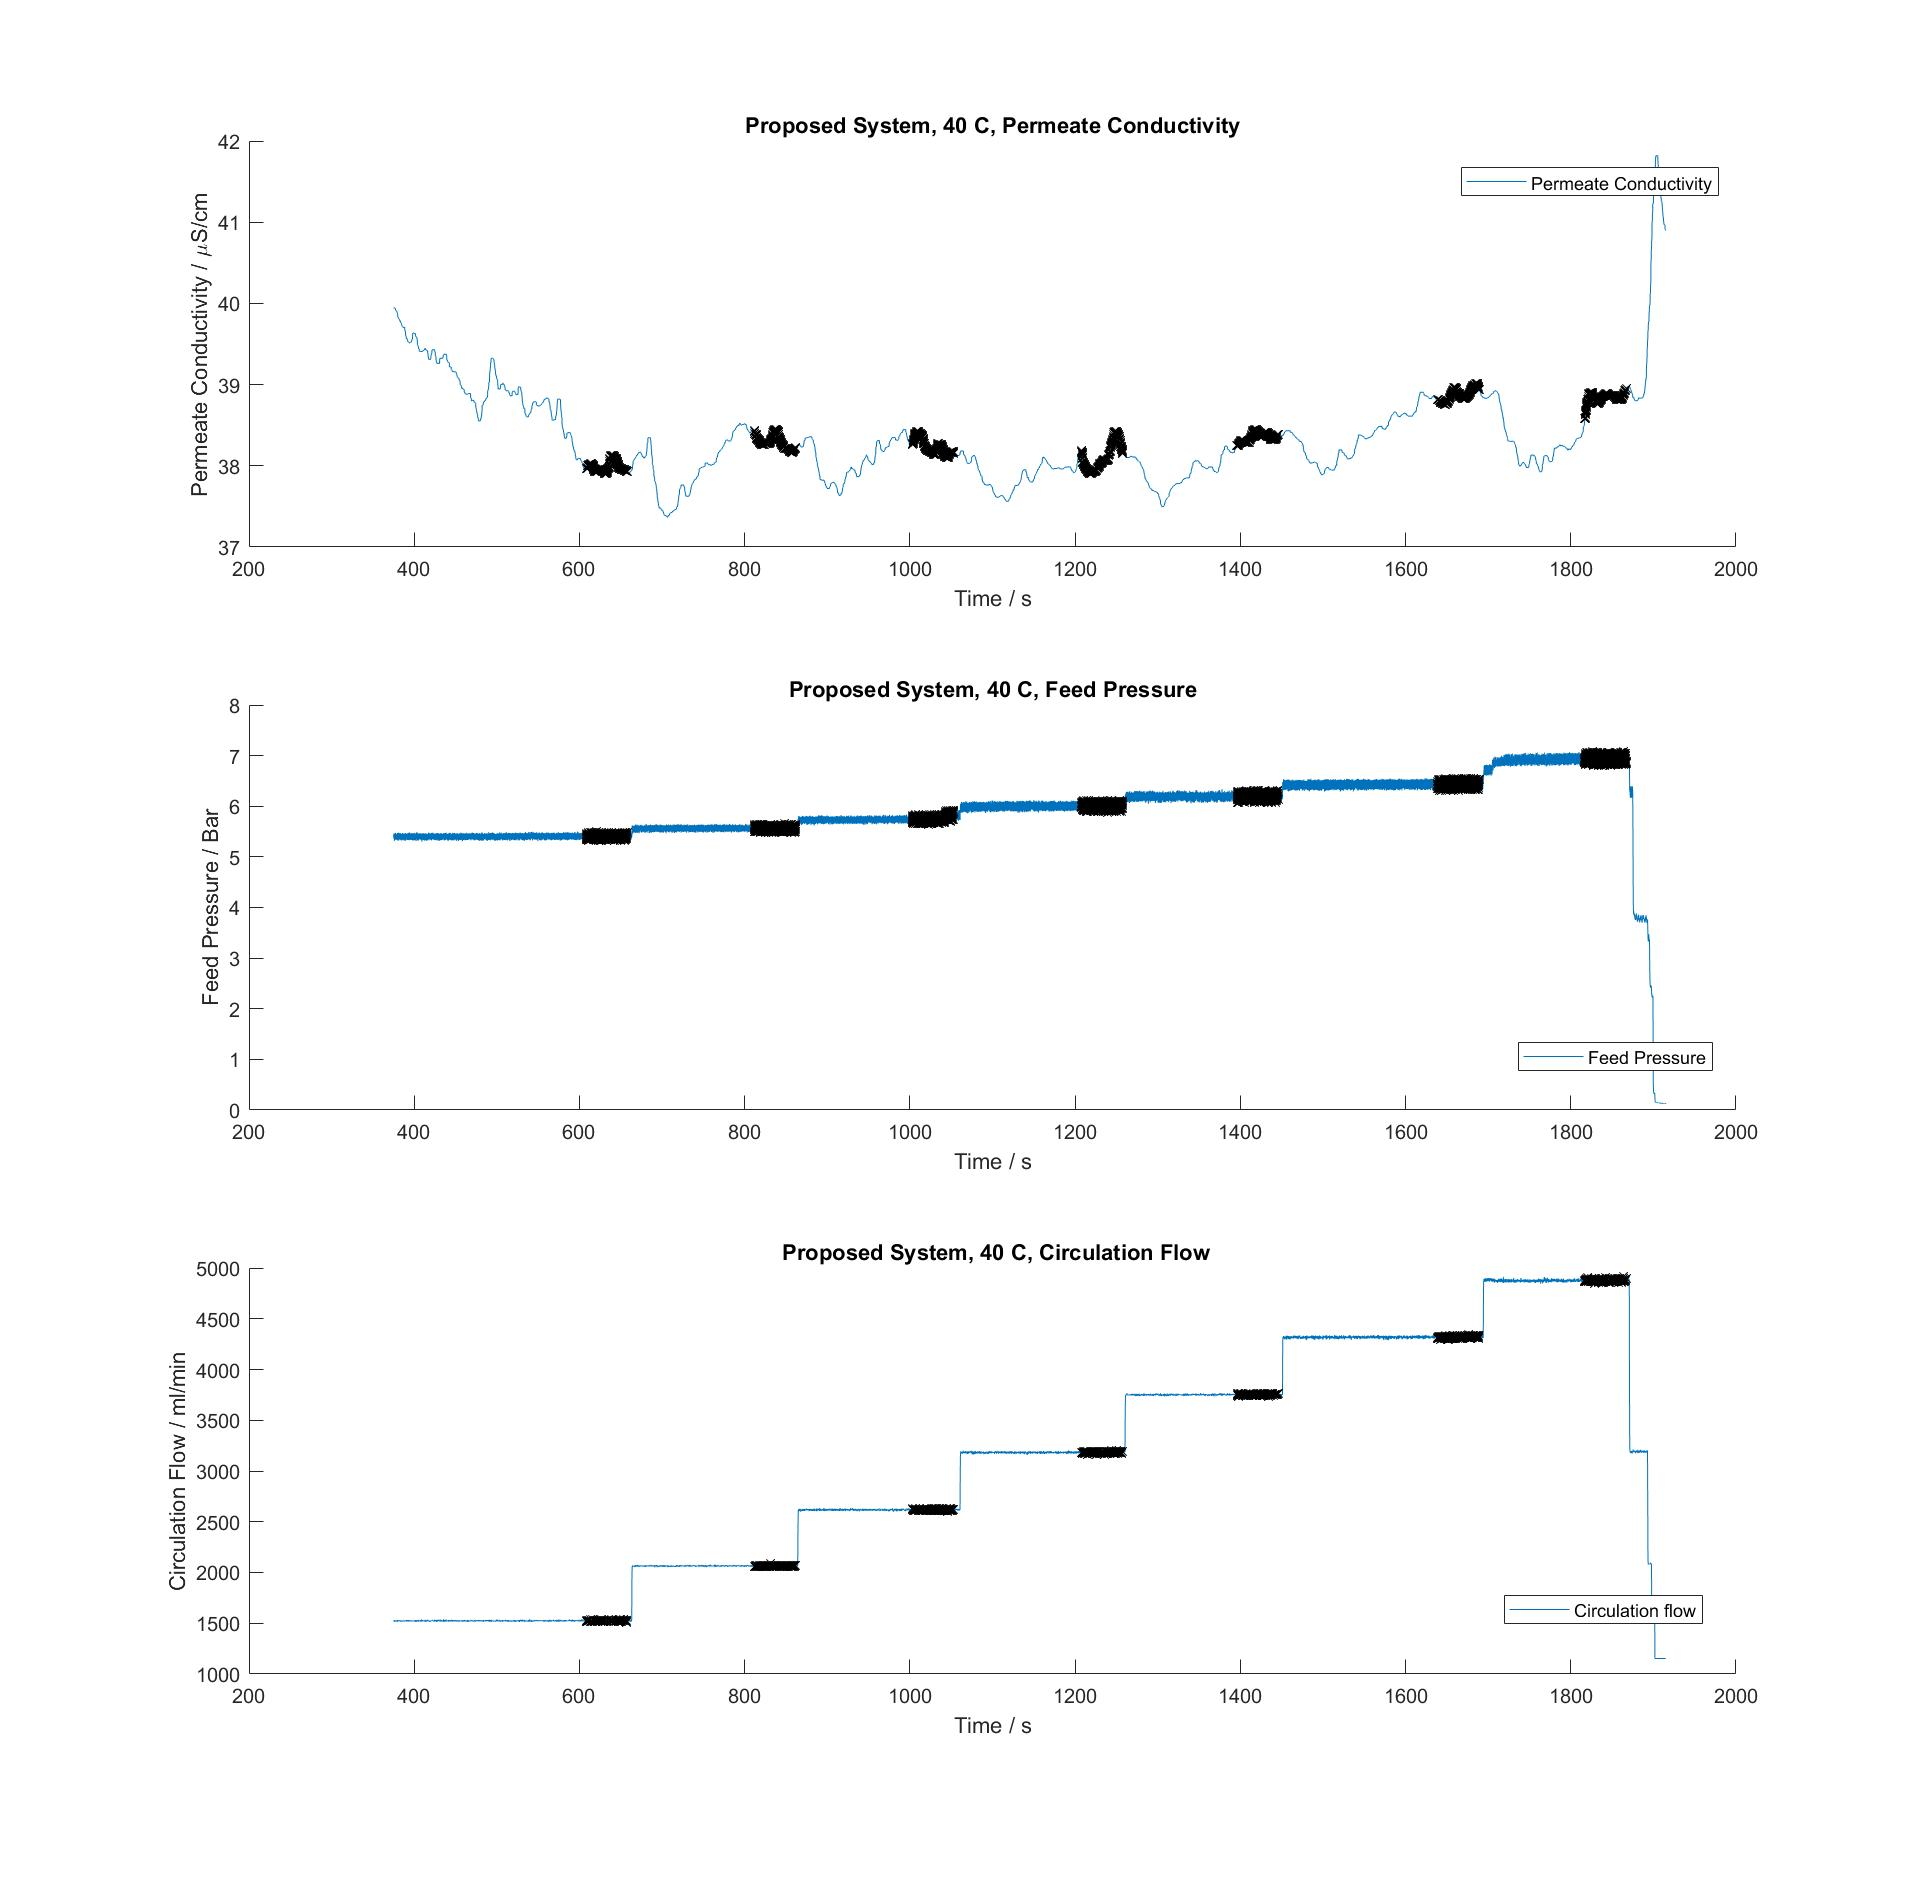
\includegraphics[width=1\textwidth]{RecIncrease40}
    \caption{Overview of test, The circulation flow was increased with the circulation pump without changing the feed pump.}
    \label{fig:RecIncrease40}
\end{figure}  
More information about how the system performed during the test was calculated and can be seen in figure \ref{fig:RecIncreaseKey40}. The Recovery decreased from 22\% to 14\%  but salt rejection and permeate conductivity did only increase slightly. \\
\\
\begin{figure}[H]
    \centering
    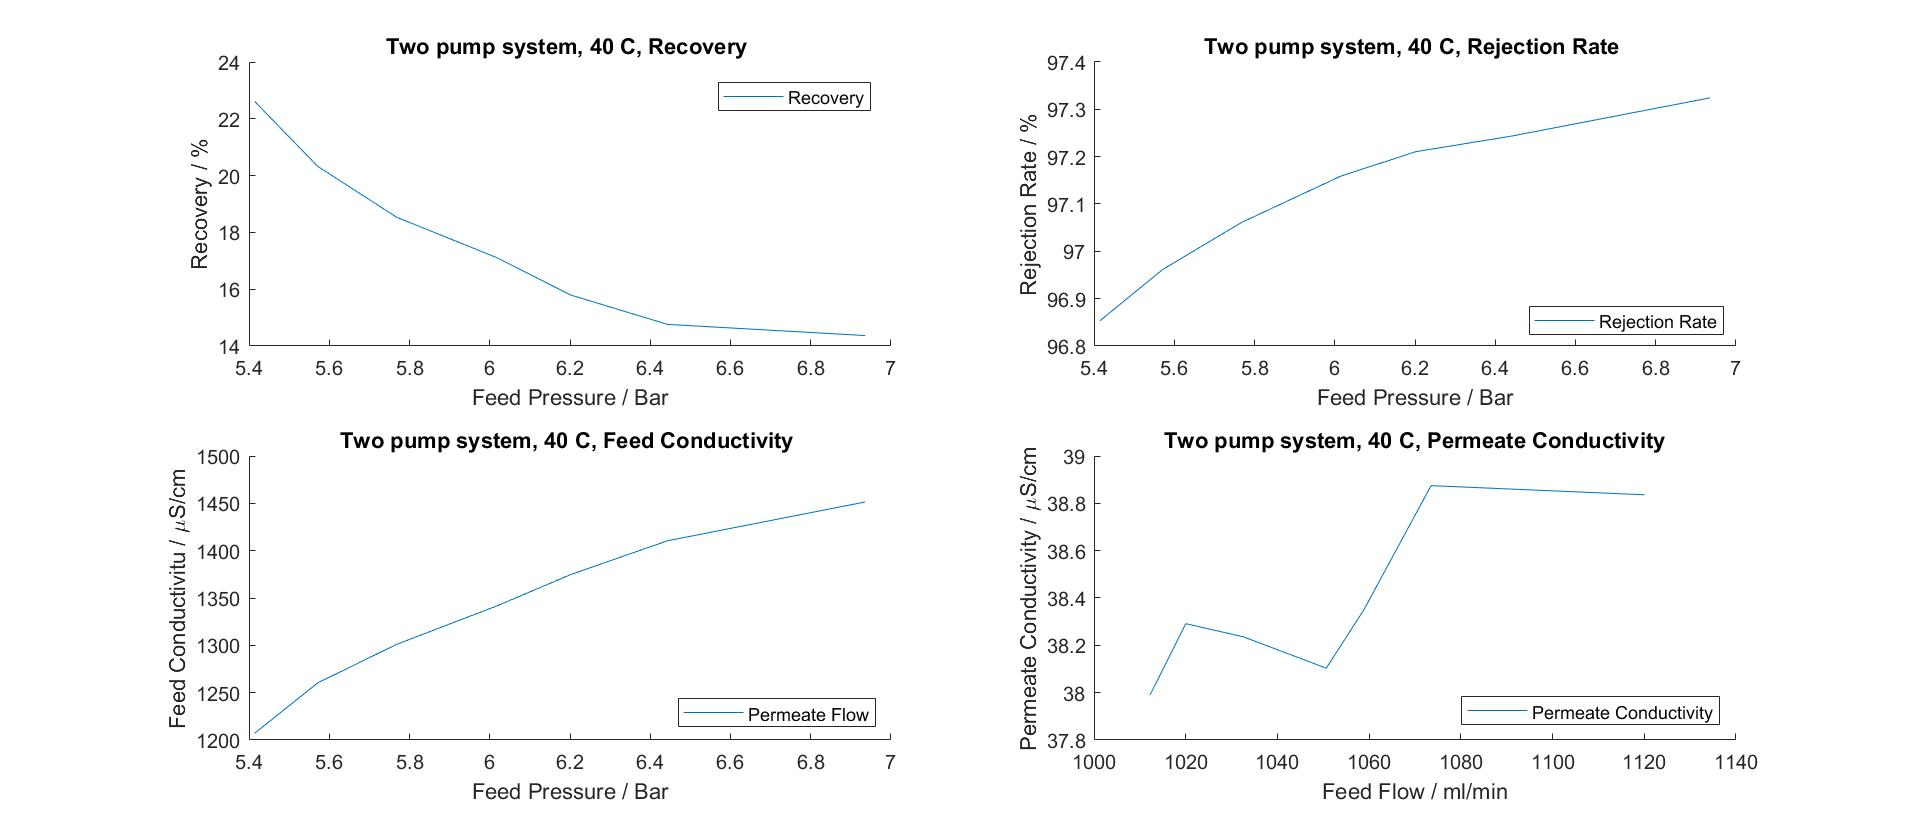
\includegraphics[width=1.1\textwidth]{RecIncrease40Key}
    \caption{The steady state measurements were used to calculate key system parameters when the circulation flow was increased}
    \label{fig:RecIncreaseKey40}
\end{figure} 
\par\bigskip 
\noindent
The test concluded that the initial theory that increased circulation flow would lead to better system performance was false. Increasing the circulation has no measurable positive effect on the system. \\
\\
\newpage
\subsubsection{Increased feed pressure}
The next test was set up to investigate the effect of an increased feed pressure. During the test all parameters were kept constant except the RPM of the feed pump. An overview of the test can be seen in figure \ref{fig:FeedPumpIncrease40} and the key parameters calculated after the test can be seen in figure \ref{fig:FeedPumpIncrease40Key}.\\
\\
\begin{figure}[H]
    \centering
    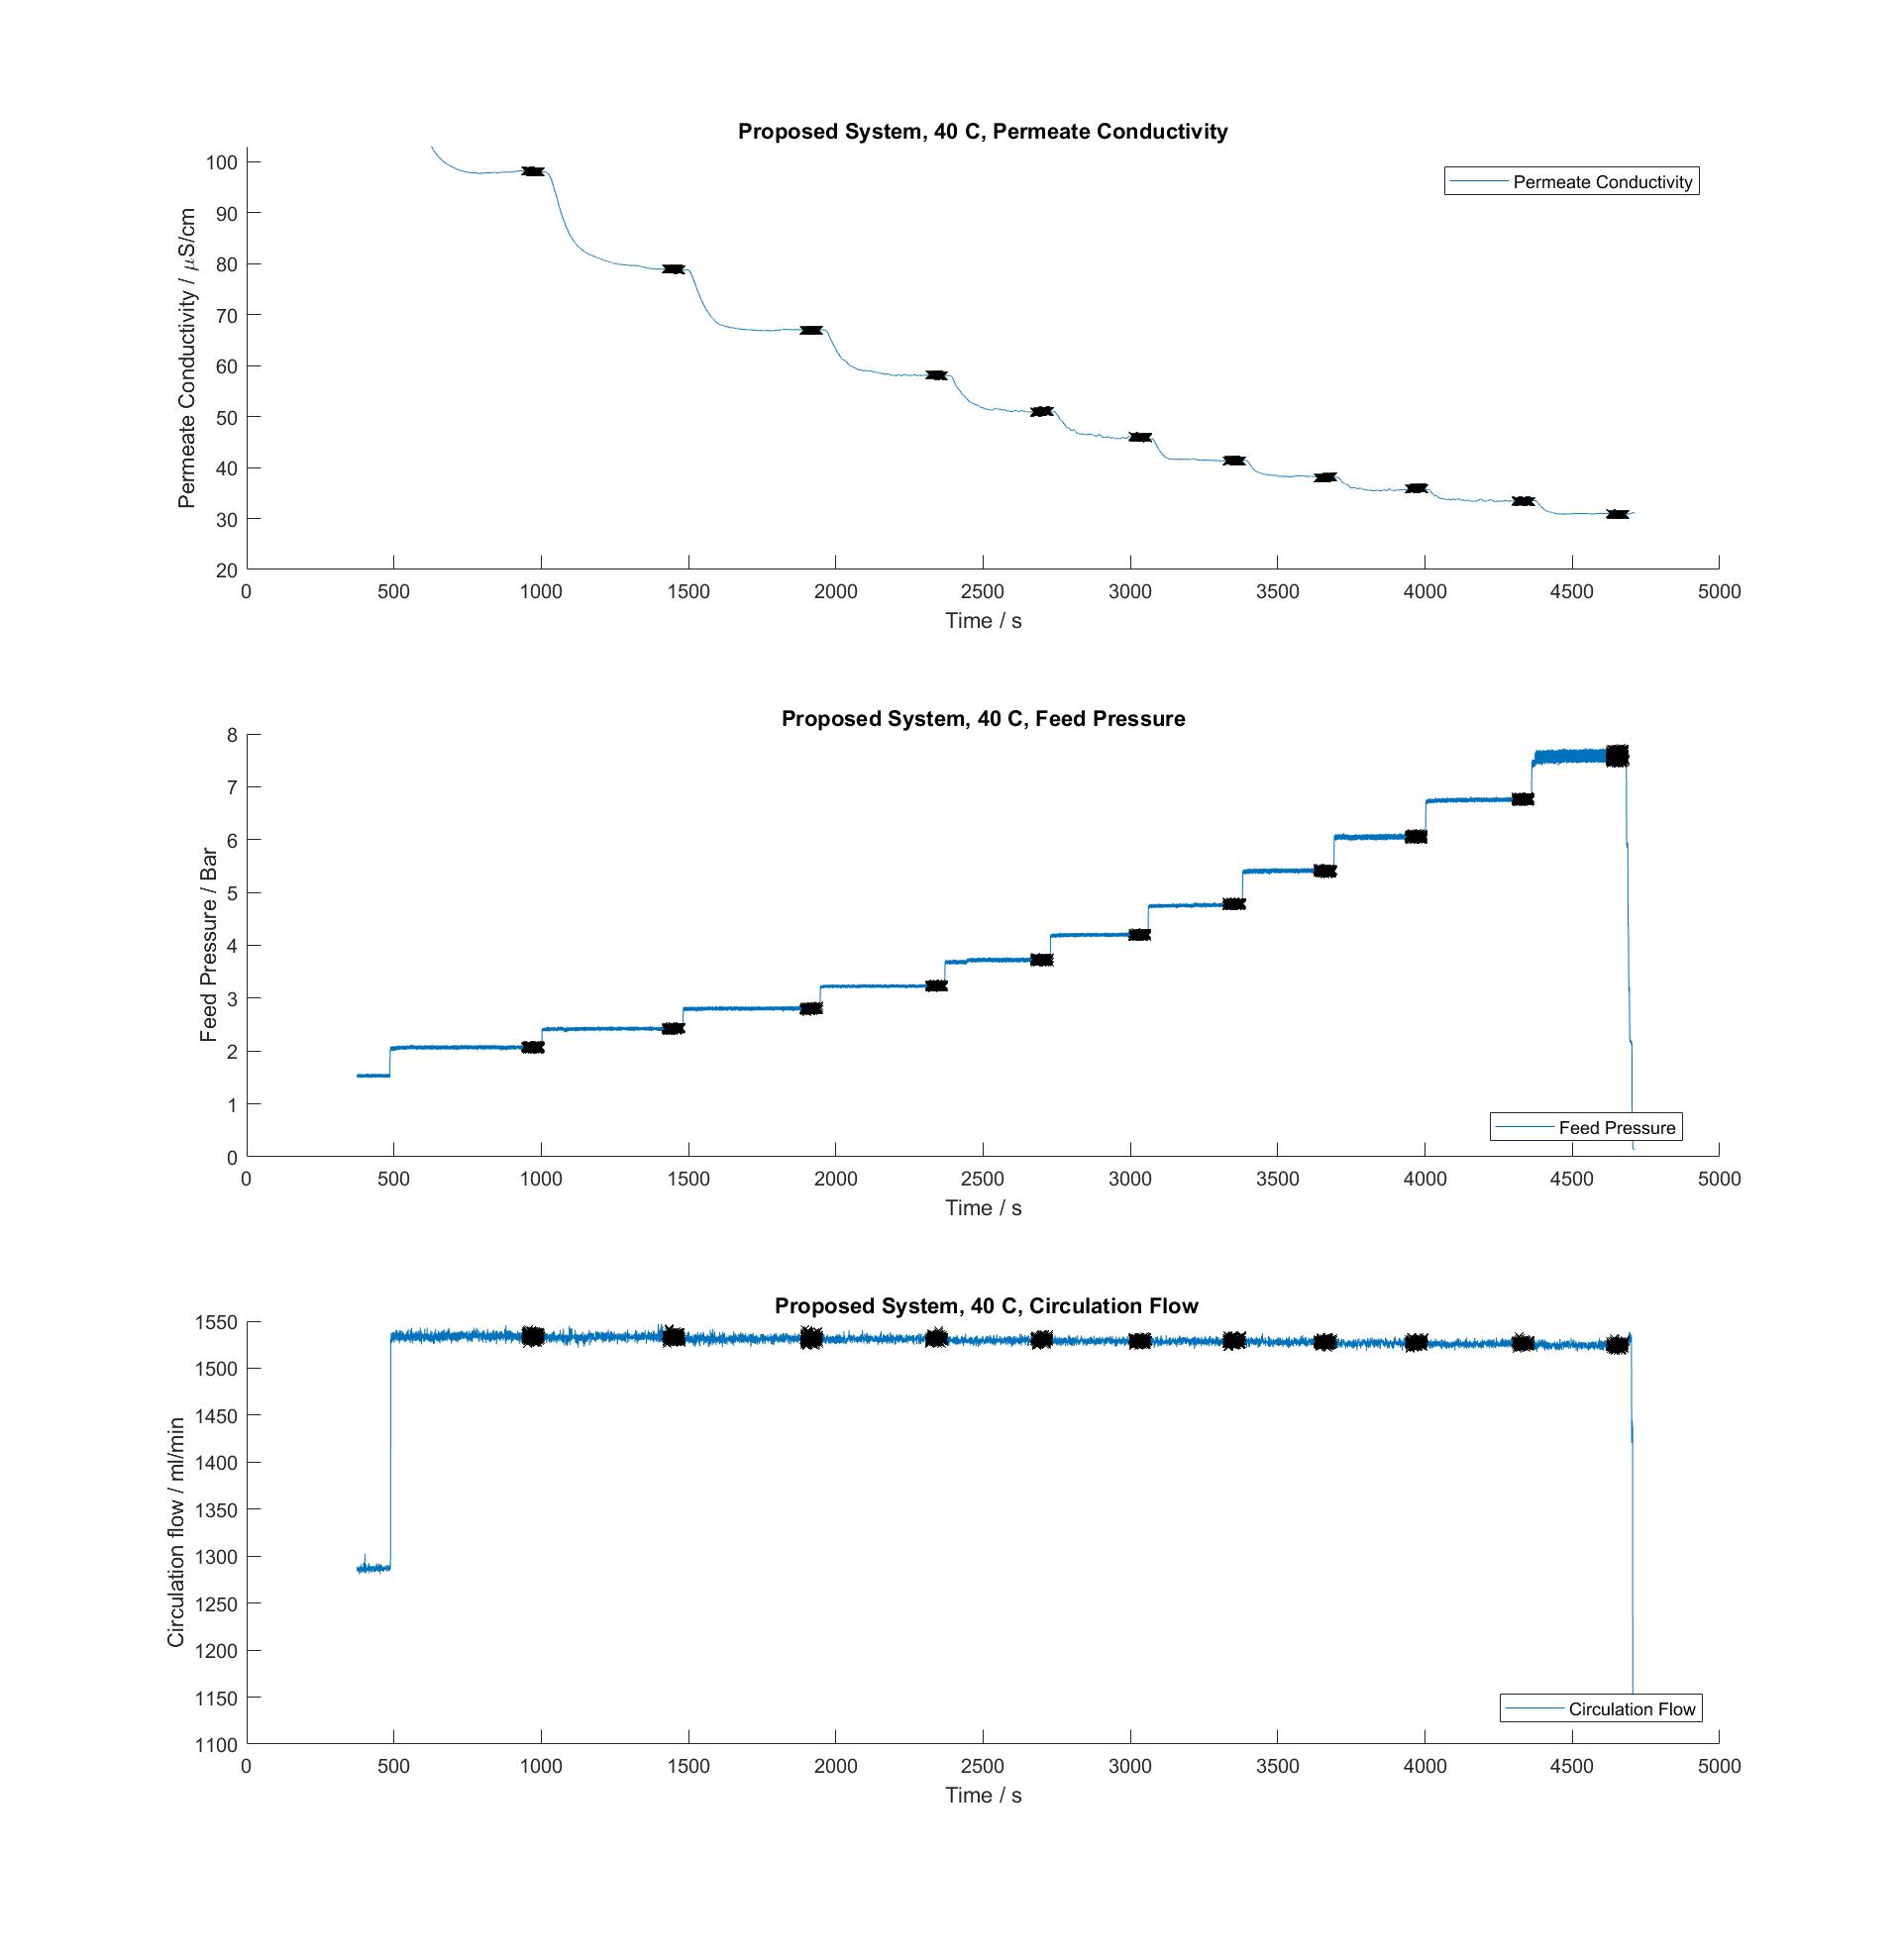
\includegraphics[width=1.1\textwidth]{FeedPumpIncrease40}
    \caption{Overview of test, feed pressure was increased with the feed pump without changing the circulation flow}
    \label{fig:FeedPumpIncrease40}
\end{figure}

\begin{figure}[H]
    \centering
    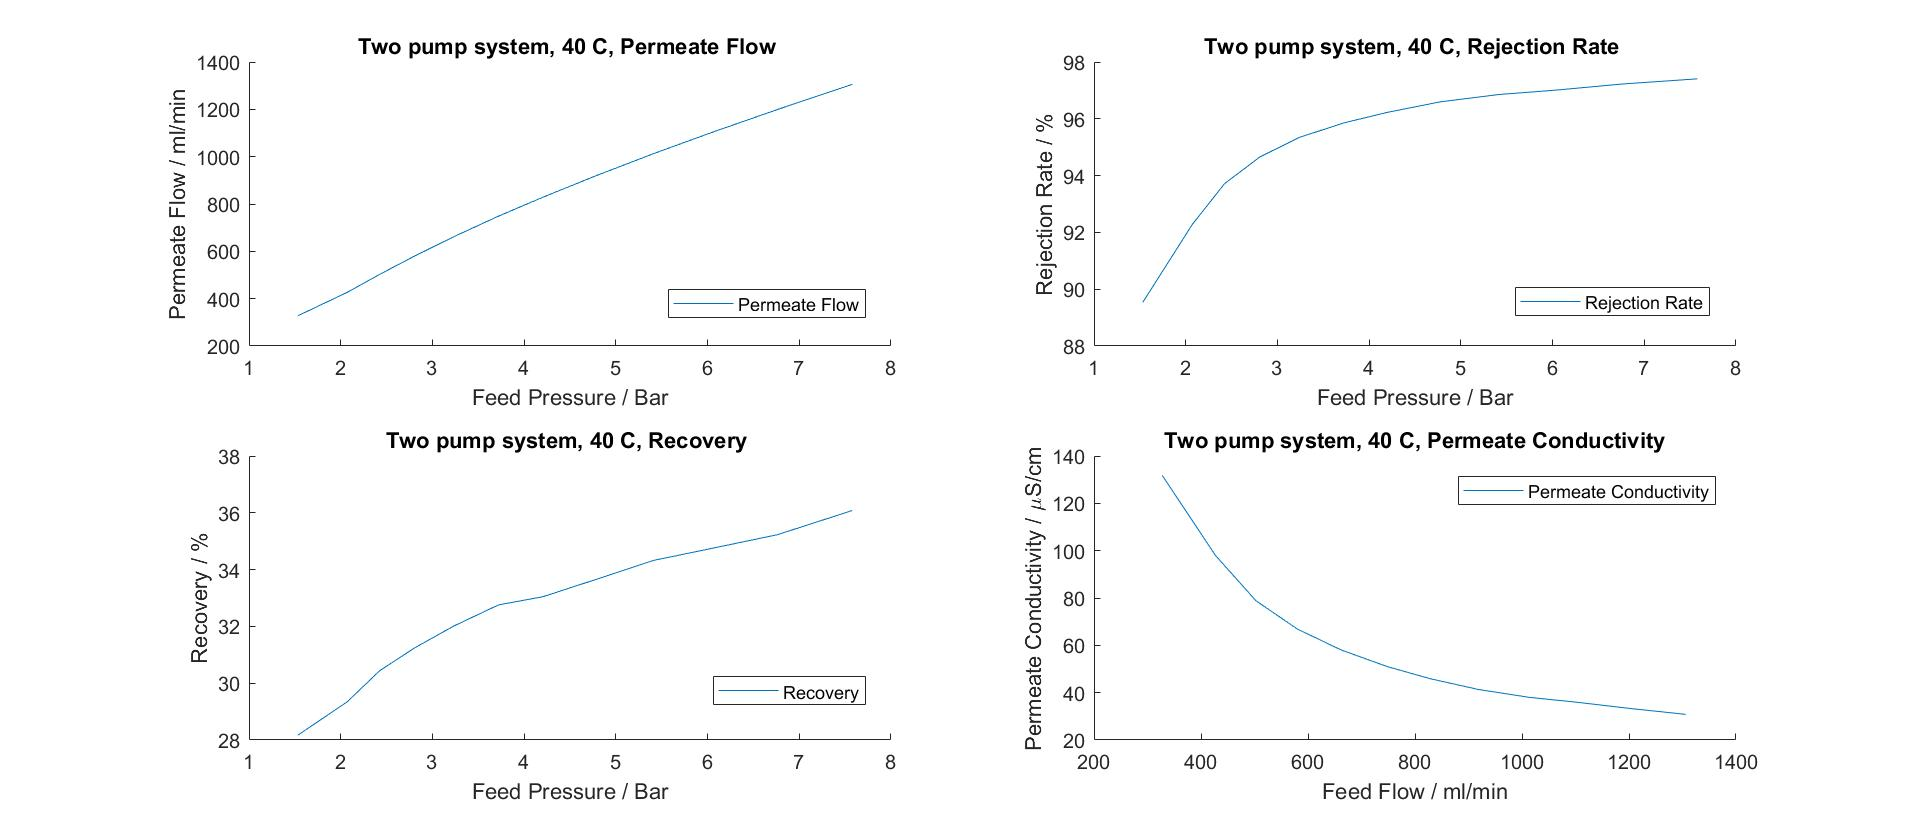
\includegraphics[width=1.1\textwidth]{FeedPumpIncrease40Key}
    \caption{The steady state measurements were used to calculate key system parameters when the feed pressure was increased}
    \label{fig:FeedPumpIncrease40Key}
\end{figure}

From figure \ref{fig:FeedPumpIncrease40} it can be seen that the circulation flow remained constant and that the feed side pressure was increased from 1.5 to 8 bars. The permeate quality increased from 100 \SI{}{\micro\siemens}/cm to 30 \SI{}{\micro\siemens}/cm. As a result, it could be concluded that it was possible to increase the performance of the membrane by increasing feed side pressure without the increased circulation flow. It should be noted that the membrane recovery increased from 28\% to 36\% during the test and this is far above the maximum limit specified by the manufacturer (20\%). Therefore, it should also be concluded that only controlling the feed pump without controlling membrane recovery could damage the membrane. 

Another important conclusion is that increasing feed pressure results in a higher salt rejection and thus more water can be recirculated instead of being rejected through the drain valve. This means that saving water will cost more energy. On the other hand if energy consumption were to be minimized salt rejection would decrease and then more water must be rejected. As a result, increased water efficiency will increase energy consumption and vice versa.  

 
\newpage
\subsection{Optimization algorithm}

Previous tests concluded that it was ineffective to increase salt rejection by increasing the circulation flow, that it was possible to increase feed side pressure to increase salt rejection and that water temperature was the parameter that had the largest deterimental effect on salt rejection. Increased feed water conductivity also decreased the performance of the system, but not as much as increased temperature and the negative effect of high conductivity was more prominent at higher temperatures. Increased feed side pressure has a larger positive effect on salt rejection at high temperature.
Since test showed that increased temperature decreased net driving pressure (See figure \ref{fig:NDP}) and that decreased feed pressure reduced salt rejection (see figure \ref{fig:SaltRejectionResult}) it could be concluded that using a fixed setpoint value at either feed side pressure or permeate flow would not work. Instead a set point could be calculated for a given temperature and pressure or permeate flow could be used as a setpoint.
By using permeate flow instead of feed side pressure as a set point, factors such as membrane fouling, scaling and individual differences in the membrane could be compensated by the controller. Therefore, permeate flow was selected to be the setpoint for the feed pump controller. 

\subsection{Finding an optimal plane}

The purpose of the next test was to find a permeate flow set point that would ensure good quality permeate at all temperatures without wasting more water and energy than needed. Since it was concluded in previous tests that membrane recovery did not improve salt rejection it was determined that this parameter should be set to approximately 20\% by controlling the circulation pump. \\
\\
The goal of the test was to find the lowest permeate flow needed at a given feed conductivity and temperature to achieve a permeate conductivity of  $\sim$ 30 \SI{}{\micro\siemens}/cm (25 to 31 \SI{}{\micro\siemens}/cm) while maintaining a recovery of at most 20\%. The test was conducted by first adjusting the temperature in the heating bath to 20 $^{\circ}$C and then add salt so that the conductivity of the water in the bath was roughly 275 \SI{}{\micro\siemens}/cm. Afterwards, the feed and circulation pump were adjusted to obtain a  permeate conductivity of  $\sim$ 30 \SI{}{\micro\siemens}/cm and 20\% recovery. Once the system had stabilised important parameters were noted. Once the measurements had been obtained, the conductivity was slowely increased and the pumps were modified to once again produce peremate water with a conductivity of 30 \SI{}{\micro\siemens}/cm. The feed conductivity was increased in small steps and the same procedure was repeated until the conductivity reached 3000 \SI{}{\micro\siemens}/cm. The same procedure was repeated using 30 $^{\circ}$C and 40 $^{\circ}$C inlet water. The raw data from the test was noted in table \ref{fig:Excel_plane}. Note that for low feed conductivities the feed pump could be set to the lowest value (3\%) and the system would still generate a permeate conductivity of less than \SI{}{\micro\siemens}/cm. If the feed conductivity was high, depending on temperature, it proved to be impossible to generate 30 \SI{}{\micro\siemens}/cm permeate. The measurements that allowed  $\sim$ 30 \SI{}{\micro\siemens}/cm permeate to be generated has been colored blue.

\begin{figure}[H]
    \centering
    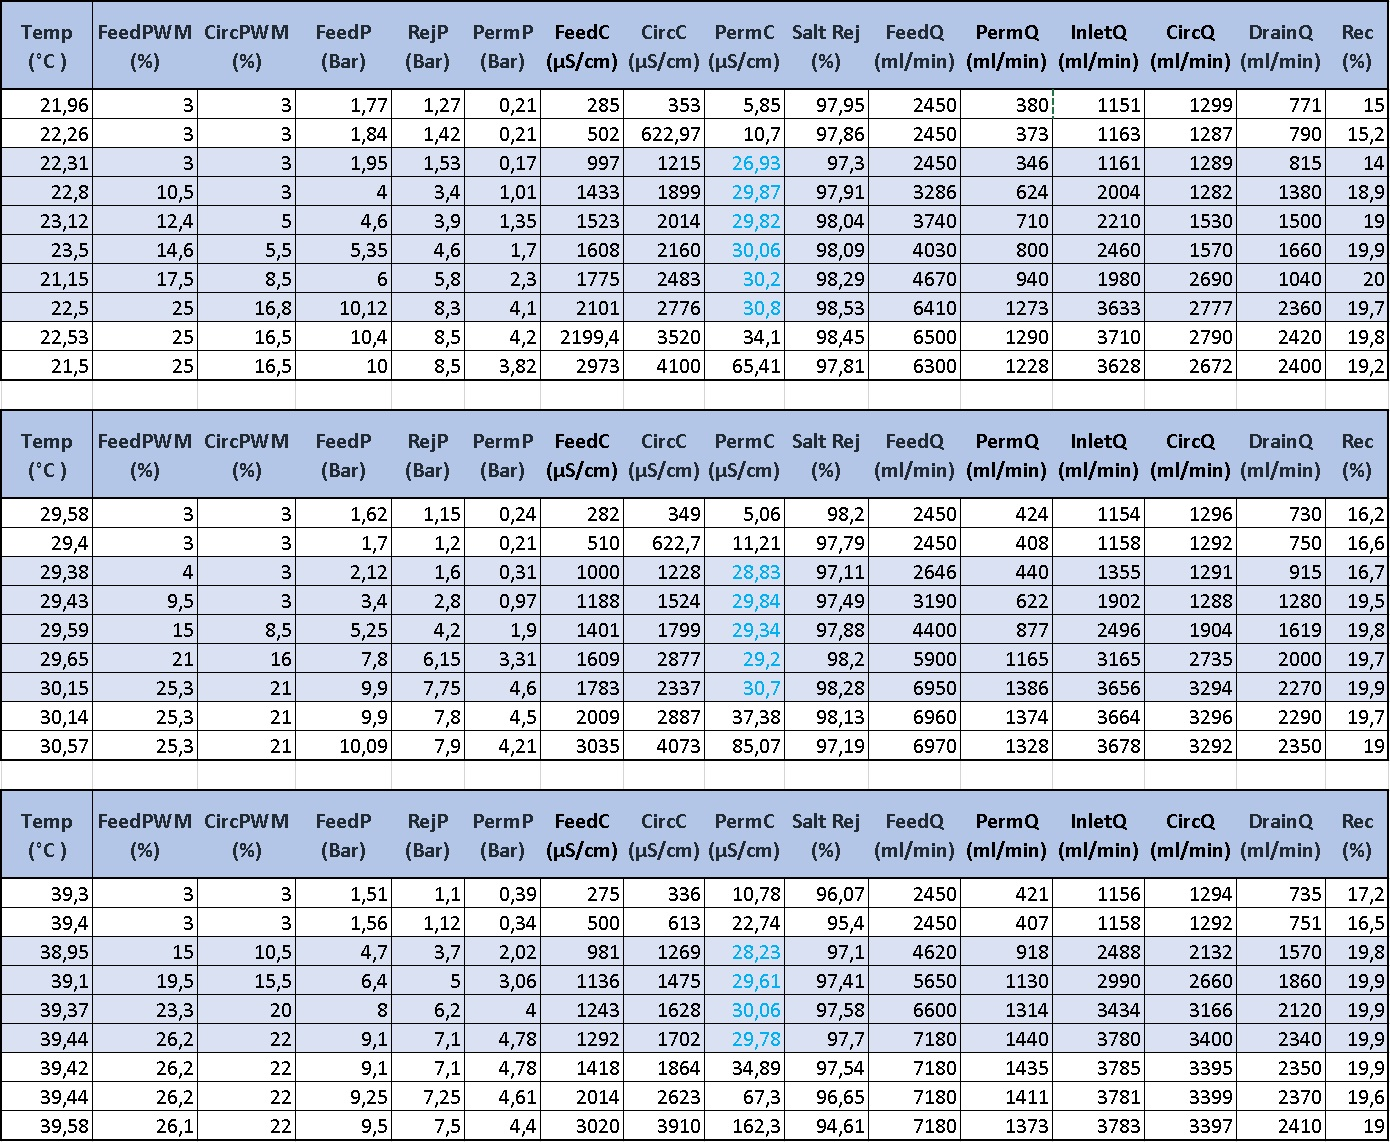
\includegraphics[width=1.1\textwidth]{Excel_plane}
    \caption{Raw data from tests at 20, 30 and 40  $^{\circ}$C. The blue cells contains information about system performance when it was possible to maintain a permeate quality of $\sim$30 uS/cm (25 - 31  \SI{}{\micro\siemens}/cm).  All relevant pressures, flows, conductivities and other key parameters has been added}
    \label{fig:Excel_plane}
\end{figure}

\newpage

By plotting when it was possible to maintain $\sim$30 \SI{}{\micro\siemens}/cm as a function of temperature and feed conductivity it was possible to estimate the working range of the membrane. Figure \ref{fig:FinalResult_1} is a 2D representation of the data contained in \ref{fig:Excel_plane}. The blue dots are the measurement points were $\sim$30 \SI{}{\micro\siemens}/cm could be maintained. As can be seen in the plot, increasing temperature limits the ability to maintain good permeate quality. The two most important findings were that at 40 $^{\circ}$C it was possible to maintain  $\sim$30 \SI{}{\micro\siemens}/cm permeate if the feed conductivity was below 1292 \SI{}{\micro\siemens}/cm and when the temperature was decreased to 20 $^{\circ}$C the feed conductivity could be increased to 2101 \SI{}{\micro\siemens}/cm and still produce  $\sim$30 \SI{}{\micro\siemens}/cm permeate.   

\begin{figure}[H]
    \centering
    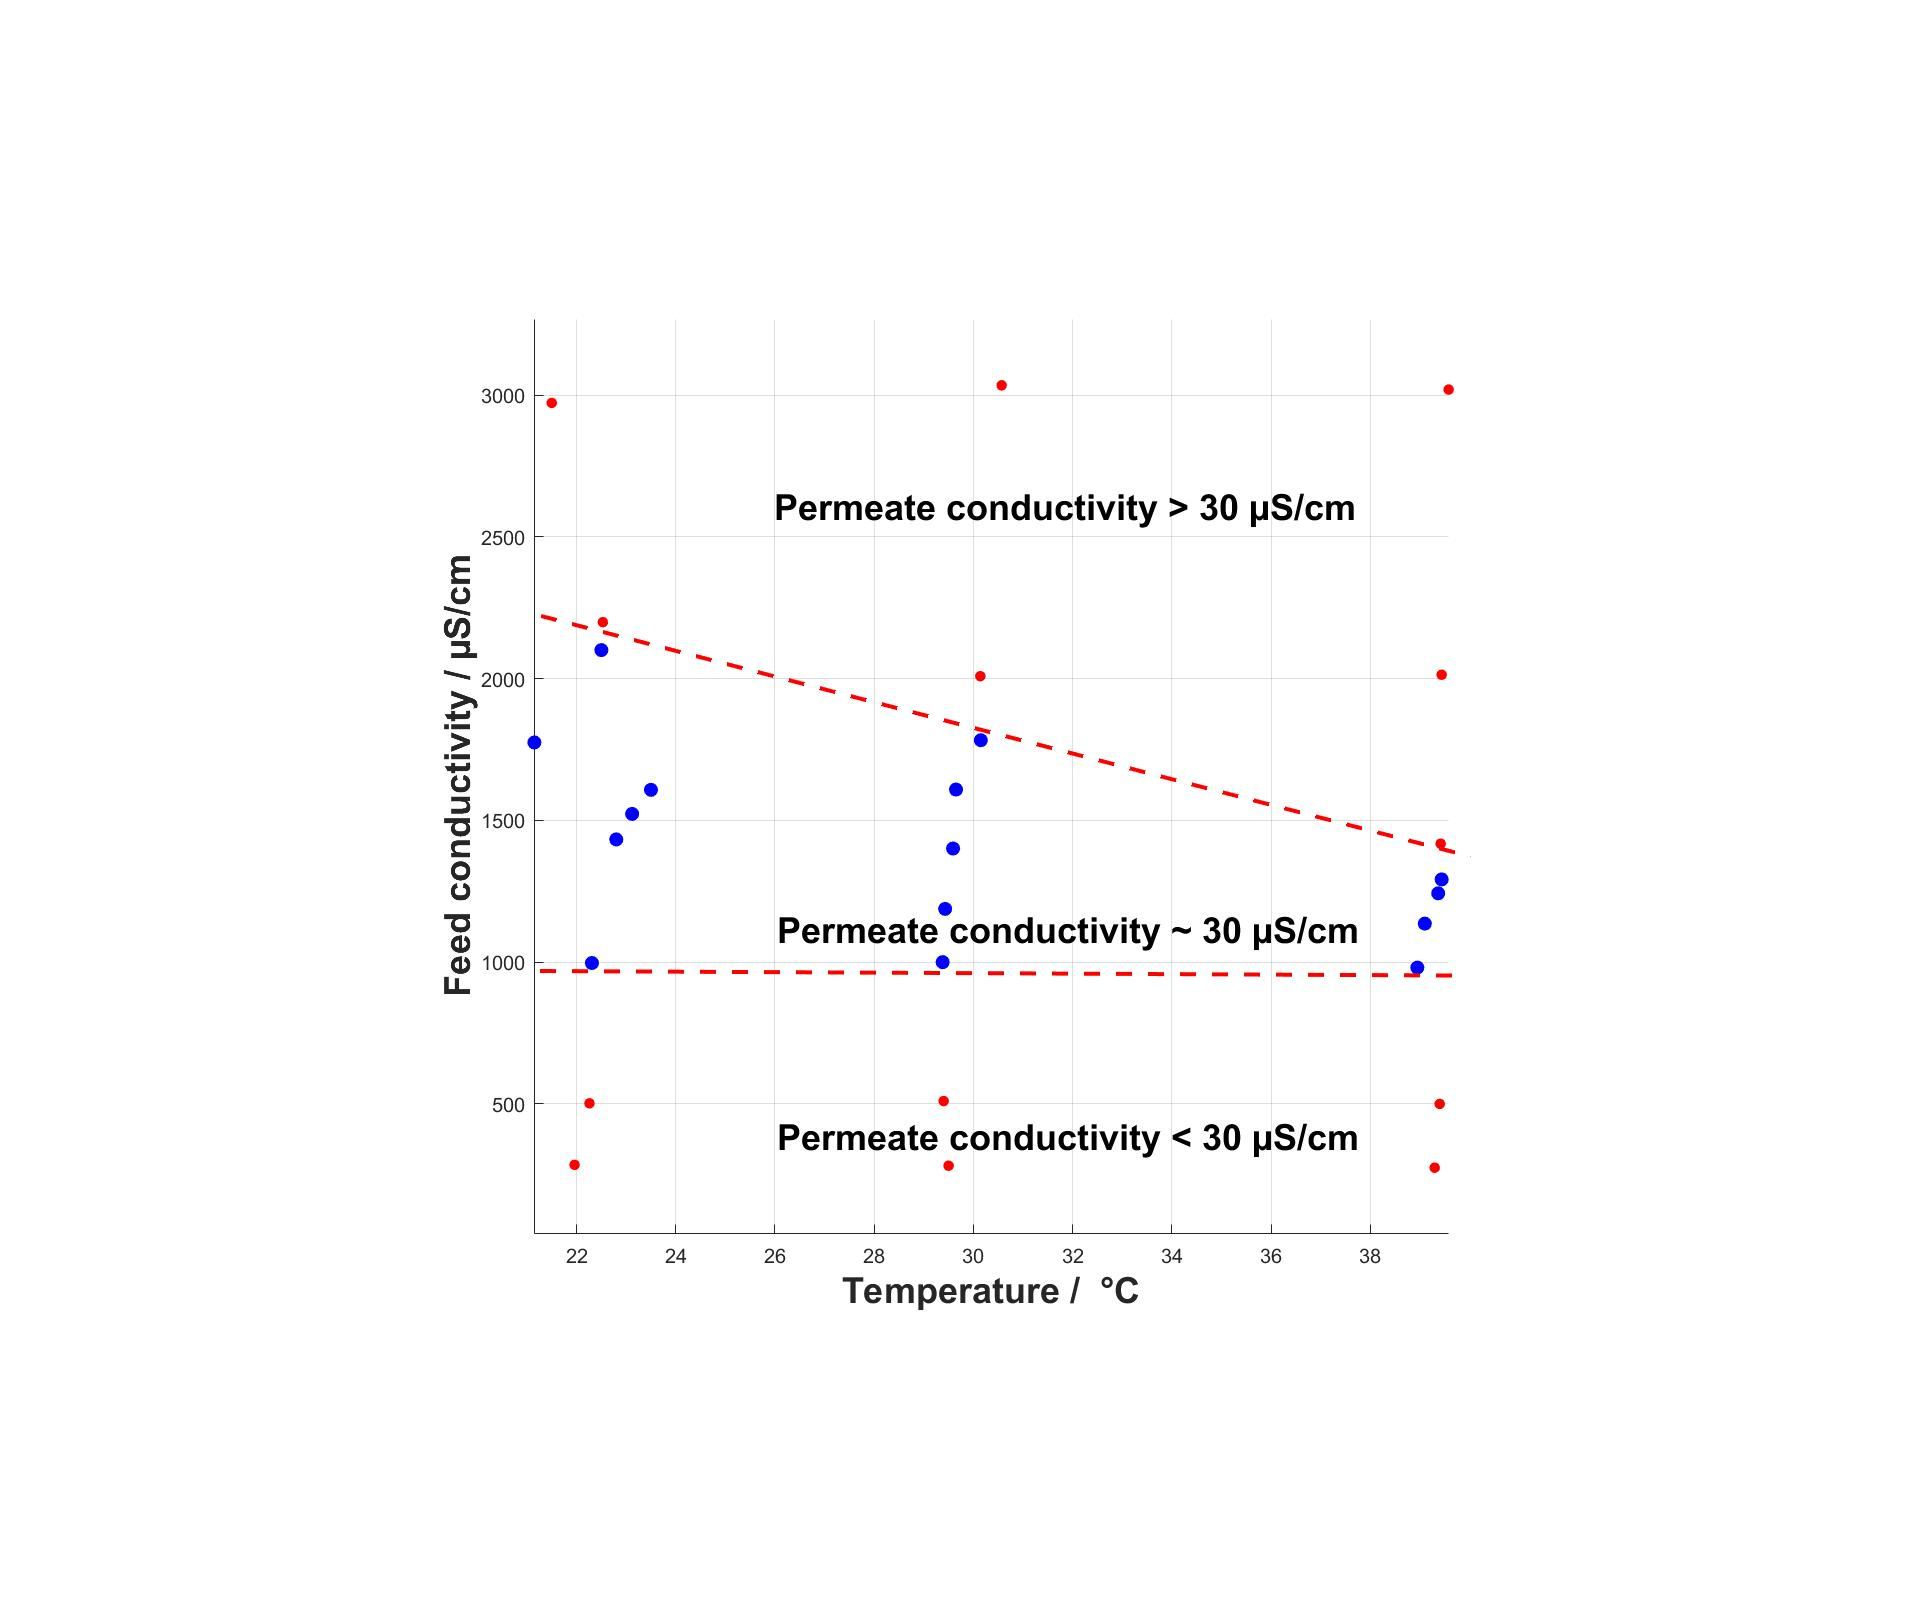
\includegraphics[width=1.1\textwidth]{FinalResult_1}
    \caption{The operational area of the membrane, blue dots represents when it was possible to generate a permeate conductivity of $\sim$30 \SI{}{\micro\siemens}/cm.}
    \label{fig:FinalResult_1}
\end{figure}

\newpage

Since the idea behind the algorithm was to find an optimal permeate flow for feed conductivities between 275-3000 \SI{}{\micro\siemens}/cm and temperatures between 20 and 40  $^{\circ}$C a Z axis containing the minimum required to achieve $\sim$ 30 \SI{}{\micro\siemens}/cm permeate flow was added to plot \ref{fig:FinalResult_1}. The blue dots represent the points where good permeate quality could be achieved. By looking at  \ref{fig:Excel_plane} it is possible to determine what permeate flow corresponds to the individual points in figure \ref{fig:FinalResult_2}.

\begin{figure}[H]
    \centering
    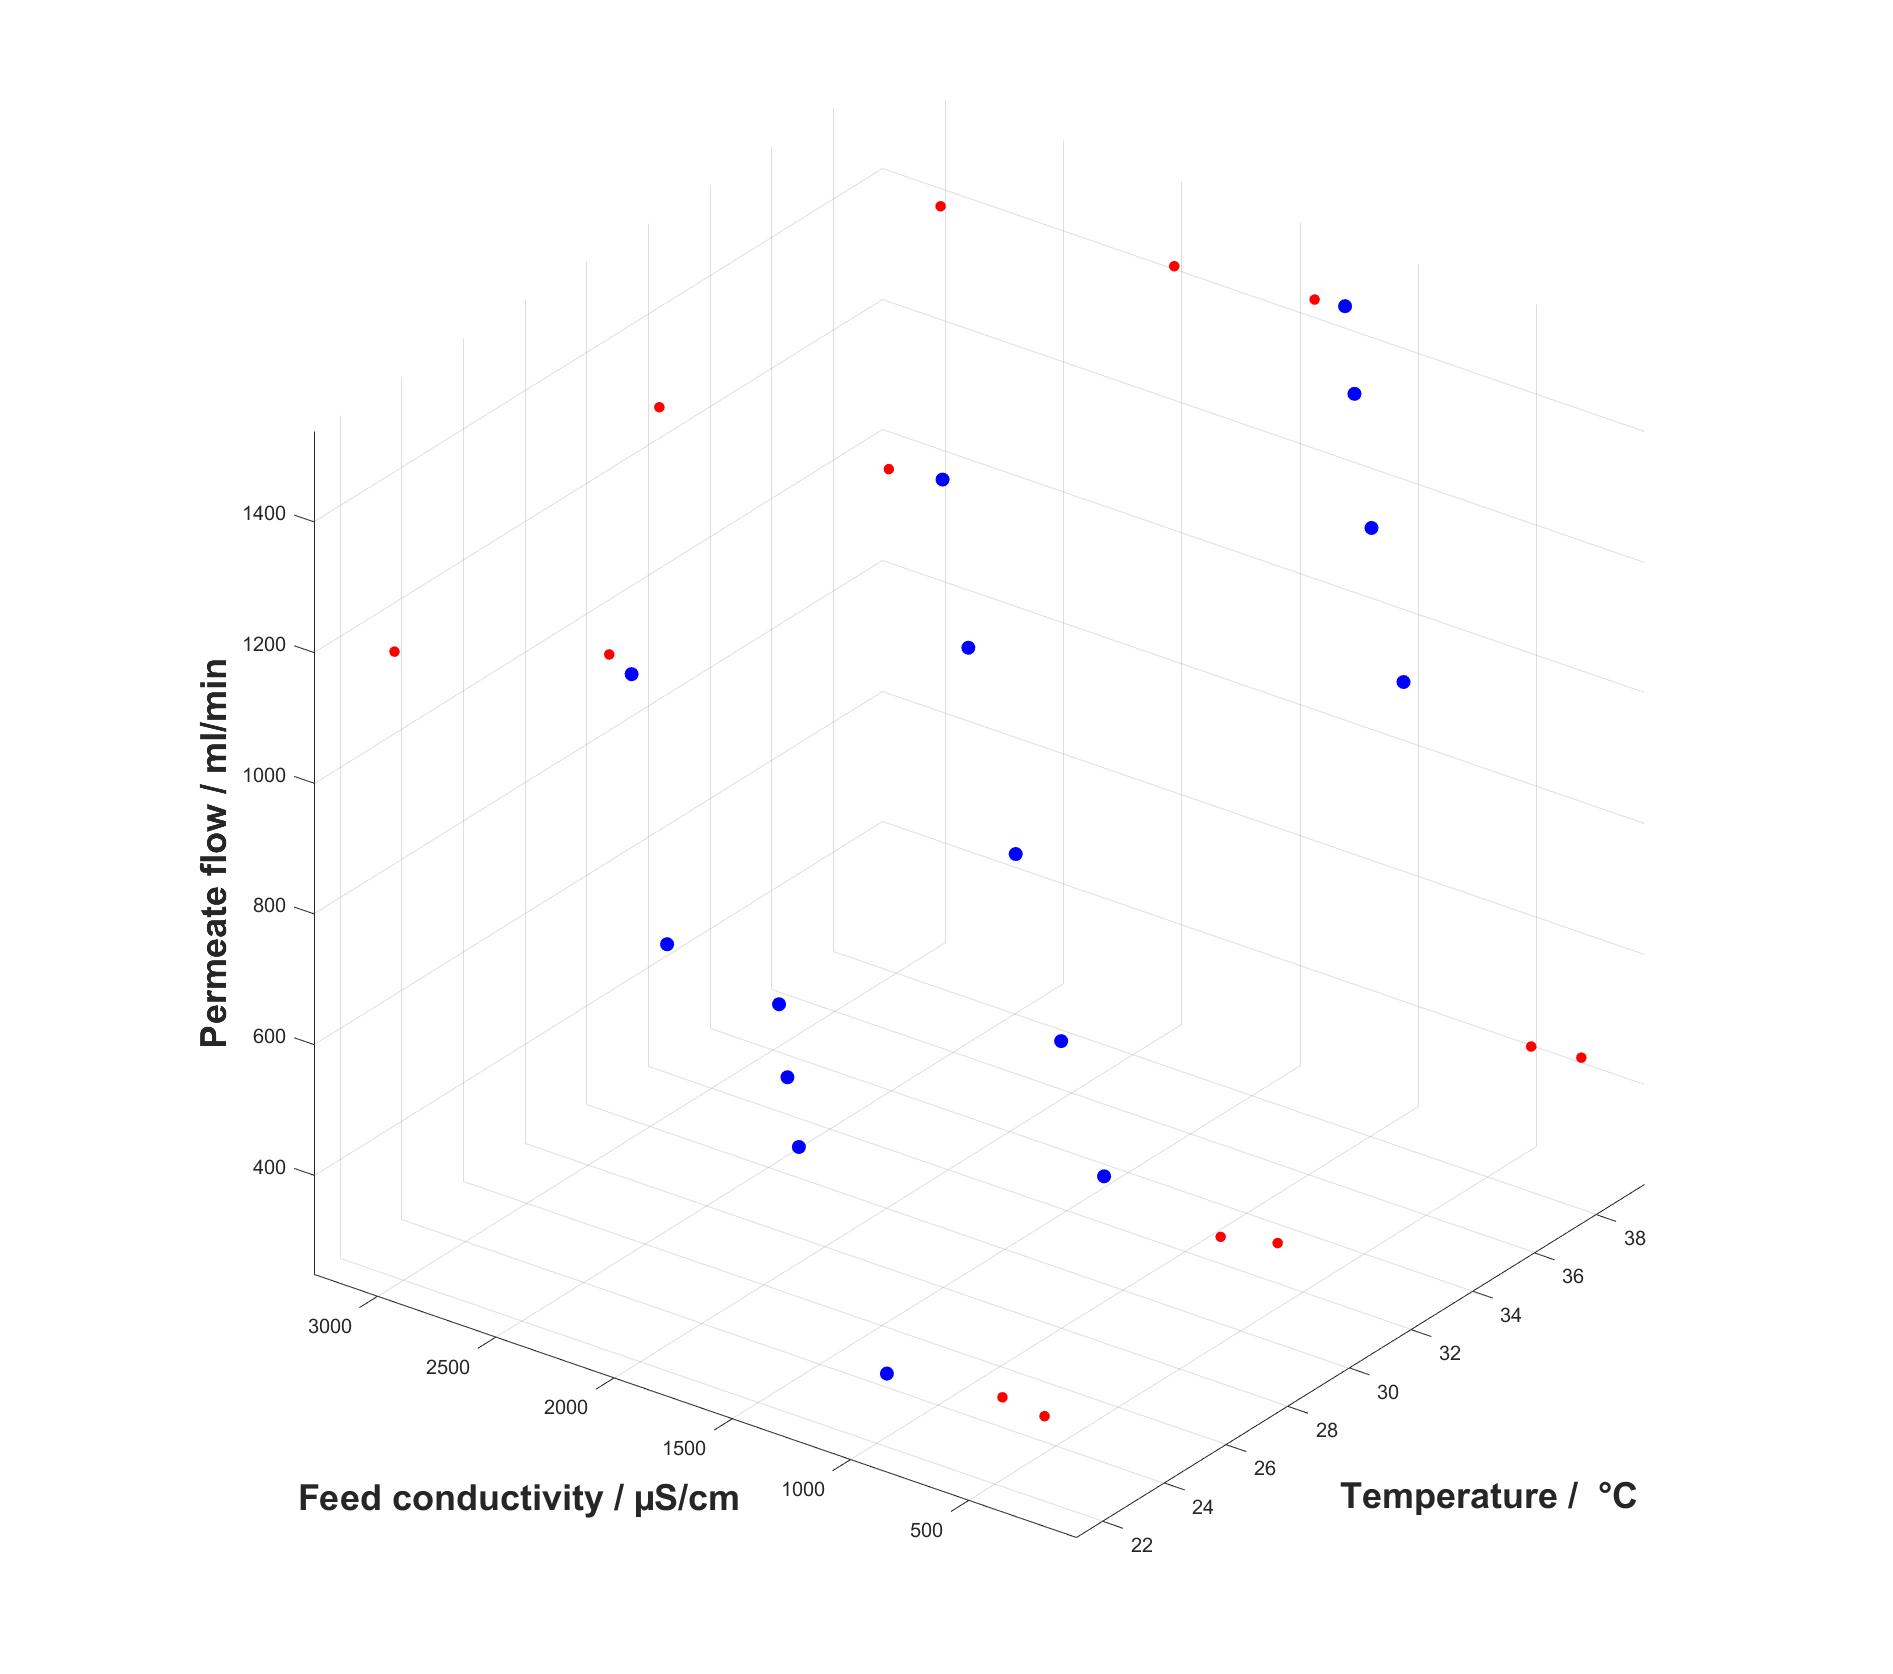
\includegraphics[width=1.1\textwidth]{FinalResult_2}
    \caption{3D representation of when it was possible to generate $\sim$ 30 \SI{}{\micro\siemens}/cm permeate as a function of temperature, feed conductivity and permeate flow.}
    \label{fig:FinalResult_2}
\end{figure}

\newpage

The points where good permeate conductivity could be attained (blue points) were used as a basis for a second order interpolation to obtain a plane. This plane can be seen in figure \ref{fig:FinalResult_3}. The plane is an estimation of what permeate flow is needed at a given temperature and conductivity to create a permeate quality of  $\sim$ 30 \SI{}{\micro\siemens}/cm. 

\begin{figure}[H]
    \centering
    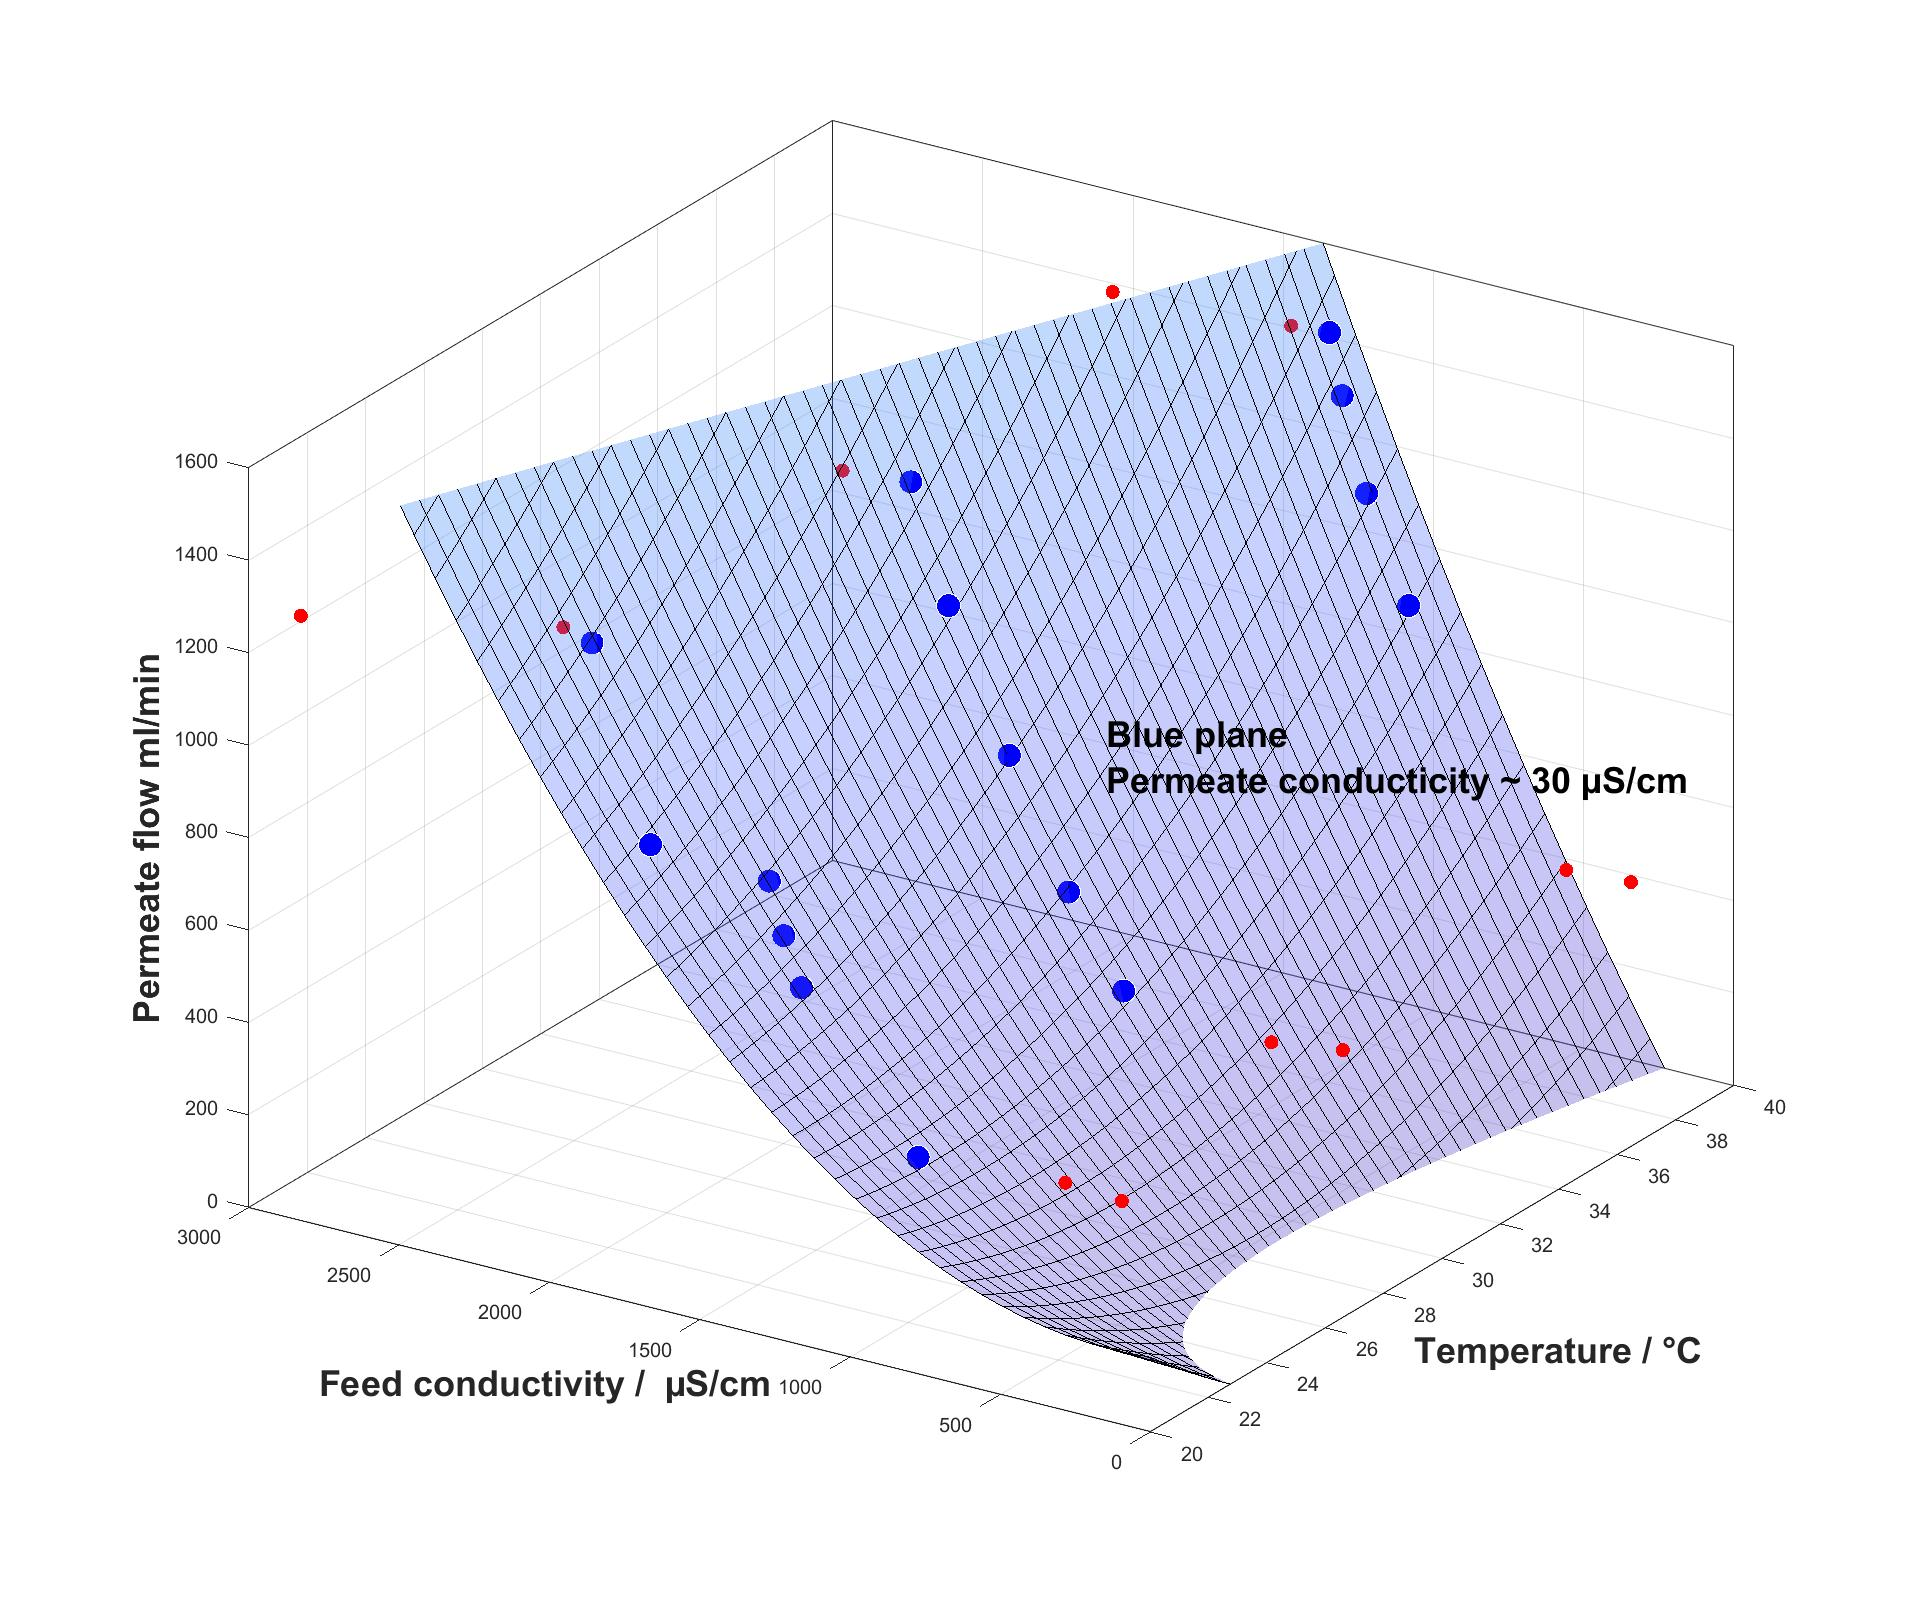
\includegraphics[width=1.1\textwidth]{FinalResult_3}
    \caption{Plane created from an interpolation of the measurements in figure \ref{fig:FinalResult_2}. The plane represents what permeate flow is needed at a given feed conductivity and temperature to generate  $\sim$ 30 \SI{}{\micro\siemens}/cm permeate}
    \label{fig:FinalResult_3}
\end{figure}

The equation for the plane can be seen below.

(temperature = t, conductivity = c)

\begin{multline}
 permeate flow =  2349-153.9*t-1.128*c+...\\
2.225*t^2+0.05315*t*c+0.0002567*c^2
\end{multline}

\newpage





Energy consumption and water efficiency is coupled in a manner such that it is imposible to minimize both at the same time. However, by selecting a curve on the aforementioned plane it is possible to find an algorithm that minimizes energy consumption without wasting more water than necessary. When the system is running at 40 $^{\circ}$C the maximum allowed conductivity that generates a permeate conductivity of  $\sim$ 30 \SI{}{\micro\siemens}/cm is limited to 1292 \SI{}{\micro\siemens}/cm. The proposed optimal function that can be seen in figure \ref{fig:FinalResult_4} was selected because it would allow the system to function at the maximum allowed conductivity at 40 $^{\circ}$C but when the system temperature decrease the system would save energy by reducing the permeate flow. For instance, if the system temperature was 40 $^{\circ}$C the function would set a permeate flow setpoint of 1440 ml/min. If the temperature was reduced to 30 $^{\circ}$C the algorithm would set the permeate flow setpoint to 767 ml/min and thereby saving energy. If the temperature was furhter reduced to 20 $^{\circ}$C the algorithm would set the permate flow setpoint to 506 ml/min. 


\begin{figure}[H]
    \centering
    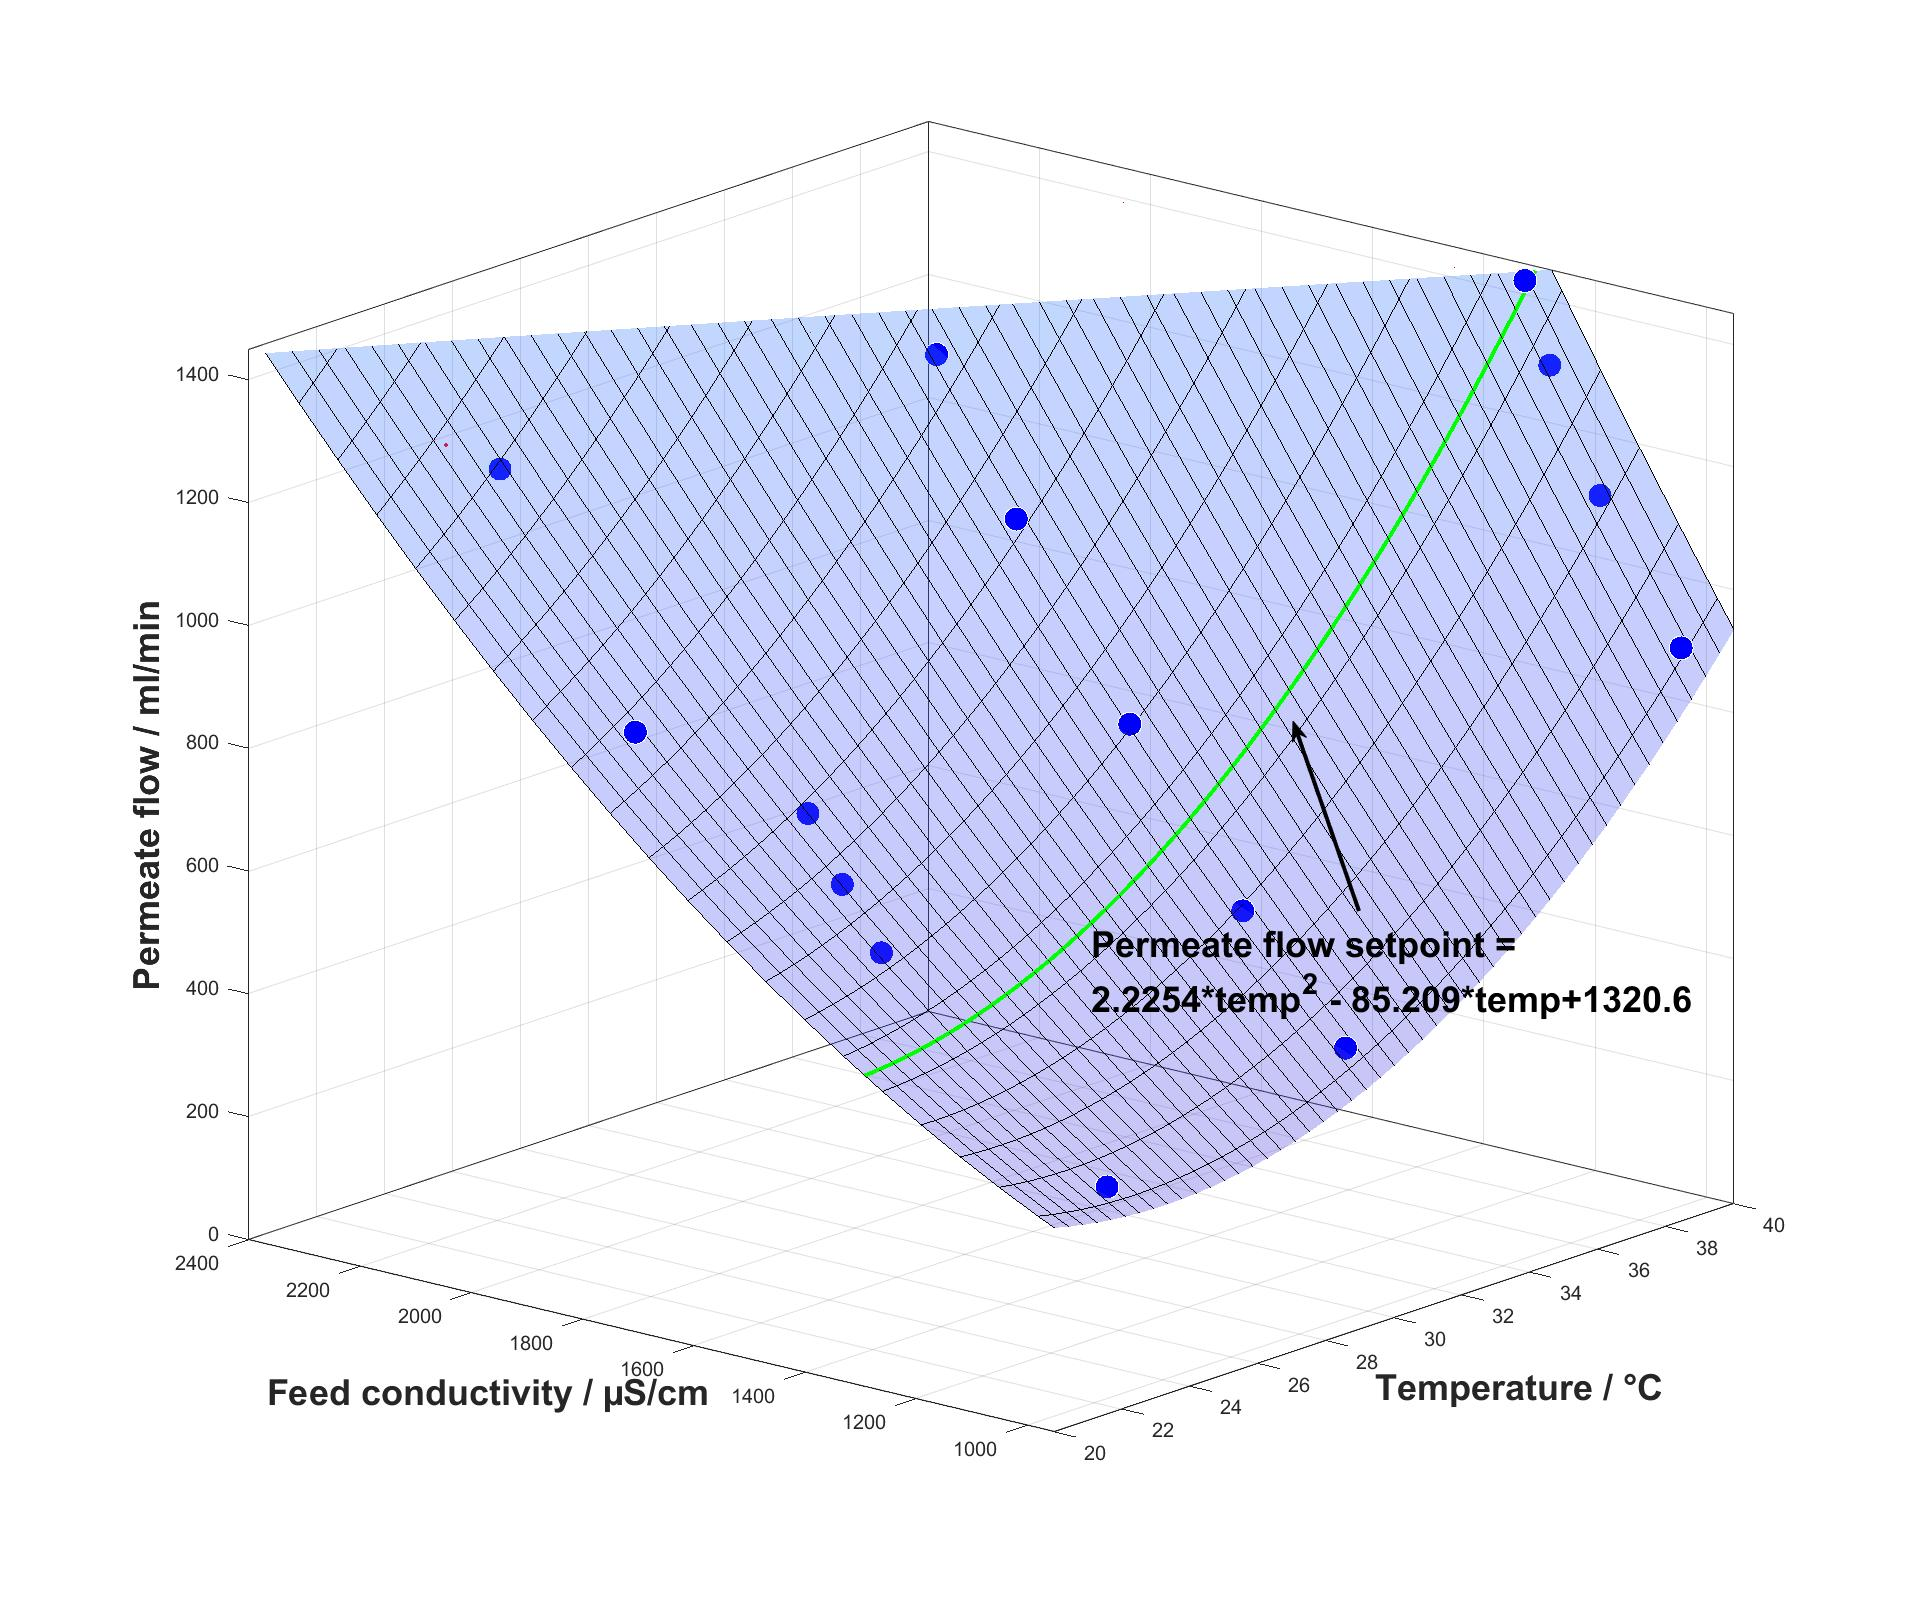
\includegraphics[width=1\textwidth]{FinalResult_4}
    \caption{The green curve represents the choosen optimization algorithm suggested in this thesis}
    \label{fig:FinalResult_4}
\end{figure}

To summarize, the proposed algorithm for optimizing the membrane is to use the temperature of the inlet water to determine an optimal permeate flow rate. By using the feed pump as the actuator one control loop controls the permeate flow to achieve the setpoint determined by the actuator. The control loop controlling the circulation pump to achieve a recovery of 20\%. The last control loop controls the drain valve so that the permeate quality is 30 \SI{}{\micro\siemens}/cm. Thus, the system will be optimized and operate on the green line in figure \ref{fig:FinalResult_4}. The proposed algorithm to calculate the optimal permeate flow based on system temperature can be seen below (temperatuer = t). Note that the function is only valid within 20 to 40 C and that the allowed permeate flow should be within 500 to 1450 ml/min. 

\begin{equation}
permeate flow =  2.2254*t^2-85.209*t+1320.6
\end{equation}

\newpage

\subsection{Energy consumption}

The current was measured on both motors during the tests with 20 $^{\circ}$C inlet water in the optimal plane test case (table \ref{fig:Excel_plane}). The test showed that power consumption of the two pump system ranged from 12 to 194.4 Watt depending on the feed conductivity and temperature which was less than what was required when only one pump was used. Typically, the one pump system used 86 Watt when running at 60\% and 228 Watt when running at 80\%. The measured power consumption of the two pump system can be seen in figure \ref{fig:EnergySys2}. \\
\\
For example, the two pump system would require somewhere between 12 and 36 Watt and the current one pump system would require 86 Watt when used in Lund (communal water, temperature 20 $^{\circ}$C, conductivity 170 uS/cm).  Since the current system does not ensure a permeate quality of 30 \SI{}{\micro\siemens}/cm it is difficult to compare the two systems. The two pump system will use more power when needed to ensure good permeate quality but the one pump system will use the same power, regardless of the permeate quality. \\
\\
Note that the feed pump generate a pressure of 10 bar when running at 25\% in the two pump system and in the one pump system the feed pump generate 7.5 bars when running at 80\%. Because of this, the two pump system can remove more of the salts than in the one pump system but it will use more energy. 

\begin{figure}[H]
    \centering
    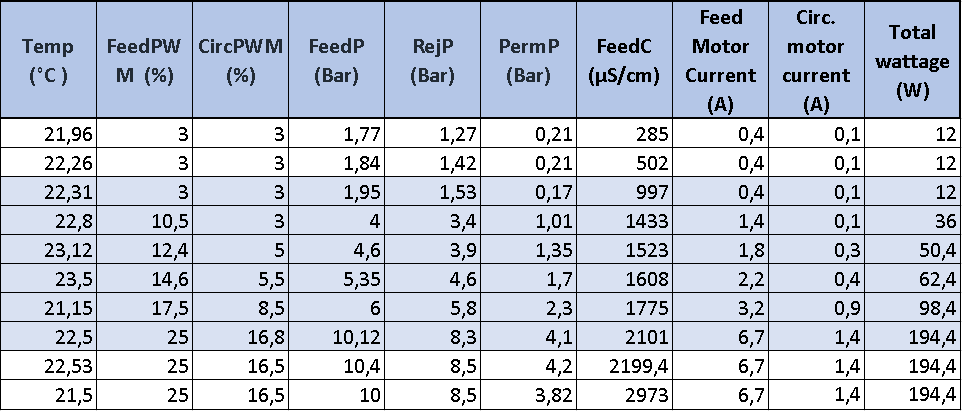
\includegraphics[width=1.1\textwidth]{EnergySys2}
    \caption{Measurements on system performance at 20 $^{\circ}$C}
    \label{fig:EnergySys2}
\end{figure}














